\documentclass[
	ngerman,
	%twoside,
	BCOR=8mm,
	headings=normal,
	parskip=half,
	headsepline,
	automark,
	listof=totoc,
	bibliography=totoc,
	%,captions=tableabove
	%draft
]{scrreprt}
%
%
%%%%%%%%%%%%%%%%%%%%%%%%%%%%%%%%%%%%%%%%%%%%%%%%%%%%%%%%%%%%%%%%%%%%%%%%%%%%%%%
% Pakete laden
%%%%%%%%%%%%%%%%%%%%%%%%%%%%%%%%%%%%%%%%%%%%%%%%%%%%%%%%%%%%%%%%%%%%%%%%%%%%%%%
%
\usepackage{ifluatex}

%
\ifluatex
 % LuaLaTeX
 \usepackage{fontspec}
 \usepackage{selnolig}
\else
 % PdfLaTeX
 \usepackage[T1]{fontenc}
 %\usepackage{lmodern}
\fi
%
\usepackage[utf8]{inputenc}
\usepackage[ngerman]{babel}
\usepackage{amsfonts}
\usepackage[ngerman]{babel}

\usepackage{csquotes}
\usepackage{scrlayer-scrpage}
\usepackage{microtype}
%
%\usepackage{ziffer}% optional
%\usepackage[locale=DE]{siunitx}% optional
%
\usepackage{tikz}
\usepackage{pgfplots}

%
\usepackage{amsmath}
\usepackage{amssymb}
%

\usepackage{url}
\usepackage{xurl}
\usepackage{breakurl}
\usepackage[breaklinks]{hyperref}


%
%=== wichtig, dass folgende Pakete NACH hyperref geladen werden ===============
\usepackage{scrhack}% Um Warnung bzgl. \float@addtolists im listings-Paket (s.u.) zu vermeiden
\usepackage{listings}

%
\usepackage[nameinlink]{cleveref}
\usepackage[all]{hypcap}
\usepackage[
	automake,
	toc,
	symbols,
	acronyms,
]{glossaries}

%Literaturverzeichnis
\usepackage{notoccite}
\usepackage[style=ieee, backend=biber, doi=true,url=true,maxcitenames=3, maxbibnames=3, sorting=none]{biblatex}

\usepackage{graphicx}
\usepackage{grffile}
\usepackage[format=plain,justification=RaggedRight,singlelinecheck=false,font={small},labelsep=space]{caption}

\usepackage{ragged2e}

\usepackage[a4paper,margin=2cm,footskip=1.2cm]{geometry}
\geometry{left=3.5cm,right=2.5cm,top=2.4cm,bottom=2.4cm}%Seitenränder
\usepackage[onehalfspacing]{setspace}%Zeilenabstand
\renewcommand{\\}{\vspace*{0.5\baselineskip} \newline}
\renewcommand*\MakeUppercase[1]{#1}	

\usepackage{changepage}
\newcommand\mycommfont[1]{\footnotesize\ttfamily\textcolor{blue}{#1}}



%\SetCommentSty{mycommfont}
%\SetKwInput{KwInput}{Input}                % Set the Input
%\SetKwInput{KwOutput}{Output}              % set the Output
\usepackage{blkarray}
\setlength{\parskip}{.8em} 
\setlength\parindent{0pt}
\newcommand{\paragraphLowDistance}[1]{\vspace{-0.3cm}\paragraph{#1}}
\newcommand{\paragraphtitle}[1]{\paragraph{#1}\hspace{0.1pt}\nopagebreak\\}
\newcommand{\paragraphtitleLowDistance}[1]{\vspace{-0.3cm}\paragraph{#1}\hspace{0.1pt}\nopagebreak}


%Code inserting
\usepackage{listings}
\usepackage{color}


% Requires package: color.
\definecolor{mediumgray}{rgb}{0.3, 0.4, 0.4}
\definecolor{mediumblue}{rgb}{0.0, 0.0, 0.8}
\definecolor{forestgreen}{rgb}{0.13, 0.55, 0.13}
\definecolor{darkviolet}{rgb}{0.58, 0.0, 0.83}
\definecolor{royalblue}{rgb}{0.25, 0.41, 0.88}
\definecolor{crimson}{rgb}{0.86, 0.8, 0.24}

\lstdefinestyle{JSES6Base}{
	backgroundcolor=\color{white},
	basicstyle=\ttfamily,
	breakatwhitespace=false,
	breaklines=false,
	captionpos=b,
	columns=fullflexible,
	commentstyle=\color{mediumgray}\upshape,
	emph={},
	emphstyle=\color{crimson},
	extendedchars=true,  % requires inputenc
	fontadjust=true,
	frame=single,
	identifierstyle=\color{black},
	keepspaces=true,
	keywordstyle=\color{mediumblue},
	keywordstyle={[2]\color{darkviolet}},
	keywordstyle={[3]\color{royalblue}},
	numbers=left,
	numbersep=5pt,
	numberstyle=\tiny\color{black},
	rulecolor=\color{black},
	showlines=true,
	showspaces=false,
	showstringspaces=false,
	showtabs=false,
	stringstyle=\color{forestgreen},
	tabsize=2,
	title=\lstname,
	upquote=true  % requires textcomp
}

\lstdefinestyle{JavaScript}{
	language=JavaScript,
	style=JSES6Base
}

\lstdefinestyle{ES6}{
	language=ES6,
	style=JSES6Base
}

\lstdefinelanguage{JavaScript}{
	morekeywords=[1]{break, continue, delete, else, for, function, if, in,
		new, return, this, typeof, var, void, while, with},
	% Literals, primitive types, and reference types.
	morekeywords=[2]{false, null, true, boolean, number, undefined,
		Array, Boolean, Date, Math, Number, String, Object},
	% Built-ins.
	morekeywords=[3]{eval, parseInt, parseFloat, escape, unescape},
	sensitive,
	morecomment=[s]{/*}{*/},
	morecomment=[l]//,
	morecomment=[s]{/**}{*/}, % JavaDoc style comments
	morestring=[b]',
	morestring=[b]"
}[keywords, comments, strings]

\lstalias[]{ES6}[ECMAScript2015]{JavaScript}

\lstdefinelanguage[ECMAScript2015]{JavaScript}[]{JavaScript}{
	morekeywords=[1]{await, async, case, catch, class, const, default, do,
		enum, export, extends, finally, from, implements, import, instanceof,
		let, static, super, switch, throw, try},
	morestring=[b]` % Interpolation strings.
}


%
%%%%%%%%%%%%%%%%%%%%%%%%%%%%%%%%%%%%%%%%%%%%%%%%%%%%%%%%%%%%%%%%%%%%%%%%%%%%%%%
% Globale Definitionen
%%%%%%%%%%%%%%%%%%%%%%%%%%%%%%%%%%%%%%%%%%%%%%%%%%%%%%%%%%%%%%%%%%%%%%%%%%%%%%%

%=== pdf Metadaten ============================================================
\hypersetup{
	pdfauthor={Janina Schroeder},
	pdftitle={Entwicklung einer webbasierten Applikation zur Bearbeitung von PDF Dateien},
	pdfsubject={Bachelorarbeit},
	pdfkeywords={
		Bachelorarbeit,
	},
	bookmarksnumbered=true,
	pdfstartview=FitH,
	hidelinks,
}

%=== Vorwort vor Literatur ====================================================
\defbibnote{mynote}{%
	Wie in \cref{sec:bib-content} erläutert, werden im Literaturverzeichnis 
	ausschließlich die Quellen angegeben, auf die im Rahmen einer Arbeit 
	tatsächlich verwiesen wird. Bitte prüfen Sie also das Literaturverzeichnis 
	Ihrer Arbeit immer dahingehend, ob alle zitierten Quellen~--~und nur
	diese~--~erfasst wurden. Dies trifft auf das nun folgende Verzeichnis
	\emph{nicht} zu; die 
	meisten der hier aufgeführten Quellen werden in dieser Vorlage nicht 
	zitiert. Es handelt sich lediglich um ein Beispiel für ein 
	Literaturverzeichnis mit Literaturempfehlungen zum wissenschaftlichen 
	Schreiben.
}

%=== Kopf-/Fusszeile definieren ===============================================
\clearpairofpagestyles
\ohead[]{\headmark}
\ofoot[\pagemark]{\pagemark}

%=== Farben definieren ========================================================
\definecolor{THRed}{RGB}{207,24,32}
\definecolor{THOrange}{RGB}{236,101,37}
\definecolor{THPurple}{RGB}{175,54,140}

%=== Einstellungen für cref ===================================================
\newcommand{\crefpairconjunction}{ und~}
\newcommand{\crefrangeconjunction}{ bis~}
\crefname{figure}{Abbildung}{Abbildungen}

%=== Einstellungen für plots ==================================================
\pgfplotsset{
	compat=newest,
	/pgf/number format/.cd,
	dec sep={\text{,}},
	1000 sep={\,},
}


%=== paar convenience Sachen definieren =======================================
\DeclareMathOperator{\sgn}{sgn}
\newcommand{\vecW}{\ensuremath{\mathbf{w}}}%
\newcommand{\ci}{\ensuremath{\mathrm{i}}}%
%
\newcommand{\tb}{\textbackslash}
%
\newcommand{\comm}[1]{\enquote{\texttt{\tb #1}}}
%
\newcommand{\param}[1]{%
	$\langle$\textrm{\textit{#1}}$\rangle$%
}

%=== Arial als Hauptschriftart ================================================
%\setsansfont{Arial}
%\renewcommand{\familydefault}{\sfdefault}

%
%%%%%%%%%%%%%%%%%%%%%%%%%%%%%%%%%%%%%%%%%%%%%%%%%%%%%%%%%%%%%%%%%%%%%%%%%%%%%%%
% Begriffe für glossaries definieren
%%%%%%%%%%%%%%%%%%%%%%%%%%%%%%%%%%%%%%%%%%%%%%%%%%%%%%%%%%%%%%%%%%%%%%%%%%%%%%%

%=== Abkürzungen ==============================================================
\newacronym{pdf}{PDF}{Portable Document Format}
\newacronym{iso}{ISO}{International Organization for Standardization}
\newacronym{pdl}{PDL}{Page Description Language}
\newacronym{rip}{RIP}{Raster Image Processor}
\newacronym{gdi}{GDI}{Graphics Device Interface}
\newacronym{pades}{PAdES}{PDF Advanced Electronic Signatures}
\newacronym{opi}{OPI}{Open Prepress Interface}
\newacronym{ceps}{CEPS}{Cisco Enterprise Print System}
\newacronym{cid}{CID}{Character Identifier Font}
\newacronym{icc}{ICC}{International Color Consortium}
\newacronym{pcs}{PCS}{Profile Connection Space}
\newacronym{xfa}{XFA}{XML Forms Architecture}
\newacronym{xml}{XML}{Extensible Markup Language}
\newacronym{xmp}{XMP}{Extensible Metadata Platform}
\newacronym{cad}{CAD}{Computer-Aided Design}
\newacronym{wysiwyg}{WYSIWYG}{What You See Is What You Get}
\newacronym{zsa}{ZSA}{Zeitstempel-Anbieter}
\newacronym{rle}{RLE}{Run Length Encoding}
\newacronym{ocr}{OCR}{Optical Character Recognition}
\newacronym{wcag}{WCAG}{Web Content Accessibility Guidelines}
\newacronym{bitv}{BITV}{Barrierefreie-Informationstechnik-Verordnung}
\newacronym{mime}{MIME}{Multipurpose Internet Mail Extension}
\newacronym{etsi}{ETSI}{European Telecommunications Standards Institute}
\newacronym{cades}{CAdES}{CMS Advanced Electronic Signatures}
\newacronym{xades}{XAdES}{XML Advanced Electronic Signatures}
\newacronym{aes}{AES}{Advanced Encryption Standard}
\newacronym{ppd}{PPD}{PostScript Printer Description}
\newacronym{ppi}{ppi}{Pixels per inch}
\newacronym{cie}{CIE}{Commission Internationale de l’Éclairage}
\newacronym{eps}{EPS}{Encapsulated PostScript}
\newacronym{dcs}{DCS}{Desktop Color Separation}
\newacronym{ascii}{ASCII}{American Standard Code for Information Interchange}
\newacronym{isa}{ISA}{Incremental Saving Attack}
\newacronym{cbc}{CBC}{Cipher Block Chaining}
\newacronym{mitm}{MITM}{Man-in-the-middle}
\newacronym{mac}{MAC}{Message Authentication Code}
\newacronym{swa}{SWA}{Signature Wrapping Attack}
\newacronym{usf}{USF}{Universal Signature Forgery}
\newacronym{ecb}{ECB}{Electronic Code Book}
\newacronym{dos}{DOS}{Denial-of-Service}
\newacronym{eea}{EEA}{Evil Annotation Attack}
\newacronym{ssa}{SSA}{Sneaky Signature Attack}
\newacronym{json}{JSON}{JavaScript Object Notation}
\newacronym{cdn}{CDN}{Content Delivery Network}
%
%\makeglossaries
\makenoidxglossaries 
\printnoidxglossaries 
\newacronym{iso}{ISO}{International Organization for Standardization}
\newacronym{pdl}{PDL}{Page Description Language}
\newacronym{rip}{RIP}{Raster Image Processor}
\newacronym{gdi}{GDI}{Graphics Device Interface}
%
\graphicspath{{images/}}
%
\addbibresource{references.bib}

\nocite{*} % listet alle Quellen (auch die nicht zitierten!)
%
%=== für schnelleres kopilieren alle ungeänderten Dateien auskommentieren =====
%\includeonly{
%	content/chapDeclaration,
%	content/abstract,
%	content/einleitung,
%	content/forschung\_technik,
%	content/chapForm,
%	content/chapGestaltung,
%	content/chapLiteratur,
%}
\includeonly{
	content/chapDeclaration,
	content/chapAbstract,
	content/chapAbkuerzungen,
	content/chapEinleitung,
	content/chapGrundlagen,
	content/chapMarktanalyse,
	content/chapApp,
	content/chapForm,
	content/chapGestaltung,
	content/chapLiteratur,
}

%List enumerations in References part
\newlist{referenceslist}{itemize}{1}
\setlist[referenceslist]{label=\textbf{[1]}}
\newcommand\itema{\item[\textbf{[2]}]}
\newcommand\itemb{\item[\textbf{[3]}]}
\newcommand\itemc{\item[\textbf{[4]}]}
\newcommand\itemd{\item[\textbf{[5]}]}
\newcommand\iteme{\item[\textbf{[6]}]}
\newcommand\itemf{\item[\textbf{[7]}]}
\newcommand\itemg{\item[\textbf{[8]}]}
\newcommand\itemh{\item[\textbf{[9]}]}
\newcommand\itemi{\item[\textbf{[10]}]}
\newcommand\itemj{\item[\textbf{[11]}]}
\newcommand\itemk{\item[\textbf{[12]}]}
\newcommand\iteml{\item[\textbf{[13]}]}
\newcommand\itemm{\item[\textbf{[14]}]}
\newcommand\itemn{\item[\textbf{[15]}]}
\newcommand\itemo{\item[\textbf{[16]}]}
\newcommand\itemp{\item[\textbf{[17]}]}
\newcommand\itemq{\item[\textbf{[18]}]}
\newcommand\itemr{\item[\textbf{[19]}]}
\newcommand\items{\item[\textbf{[20]}]}
\newcommand\itemt{\item[\textbf{[21]}]}
\newcommand\itemu{\item[\textbf{[22]}]}
\newcommand\itemv{\item[\textbf{[23]}]}

%
%==============================================================================
%
\begin{document}


%
\pdfbookmark[0]{Titelseite}{titel}
\begin{titlepage}
	\begin{center}
		\begin{tikzpicture}
			\fill[THRed] (0, 0) rectangle (\textwidth/3, 3pt);
			\fill[THOrange] (\textwidth/3, 0) rectangle (2*\textwidth/3, 3pt);
			\fill[THPurple] (2*\textwidth/3, 0) rectangle (\textwidth, 3pt);
		\end{tikzpicture}
	\end{center}

	\begin{huge}
		\noindent
		
		Entwicklung einer webbasierter Applikation zur \newline Bearbeitung von PDF-Dateien\\
	\end{huge}
	Bachelorarbeit zur Erlangung des Bachelor-Grades \newline
	\textit{(Bachelor of Science)} im Studiengang Technische Informatik \newline
	an der Fakultät für  Informations-, Medien- und Elektrotechnik \newline
	der Technischen Hochschule Köln \\
	~\\
	~\\
	~\\
	\noindent\begin{tabular}{ll}
		vorgelegt von: & Janina Schroeder \\
		Matrikel-Nr.: &	11132206 \\
		Adresse: & Laurentiusweg 10 \\
		~ &	50321 Brühl \\
		~ &	janina\_jessika\_jelena.schroeder@smail.th-koeln.de \\
		~ & ~ \\
		eingereicht bei: & Prof. Dr. Chunrong Yuan \\
		Zweitgutachter/in: & Prof. Dr. René Wörzberger
	\end{tabular}	
	~\\
	~\\
	Köln, 28.02.2024
\end{titlepage}
\cleardoublepage
\pagenumbering{Roman}
\chapter*{Bachelorarbeit}
\label{chap:abstract}
%
\textbf{Titel:} Entwicklung einer webbasierter Applikation zur Bearbeitung von PDF\\ Dateien

\textbf{Gutachter:}
\par
- Prof. Dr. Chunrong Yuan
\par
- Prof. Dr. René Wörzberger

\textbf{Zusammenfassung:} Für die Bachelorarbeit habe ich eine Open Source offline Webseite zur Bearbeitung von PDF Dateien im Firefox Browser programmiert. Seit Adobe den PDF Standard entwickelt hat, tauchten zahlreiche meist kostenpflichtige PDF Anwendungen, um PDF Dateien zu bearbeiten auf dem Markt auf. Ich habe den Markt an PDF Programmen analysiert und diese mit meiner Webapplikation verglichen. Daraufhin beleuchte ich den aktuellen Stand der Technik des PDF Standards. Im späteren Verlauf erkläre ich die Implementierung meiner Webapp und meine Erfahrungen mit anderen Browsern, sowie auf MacOS, Linux, Android und iOS. Die Javascript Libraries PDF.js und PDF-LIB sind das tragende Fundament meiner PDF Webapp. Die PDF Webapp vereint alle Funktionalitäten, die man für gängige PDF Bearbeitung benötigt. Man kann PDFs lesen, splitten, mergen, erstellen, sowie mit Texten, Bildern, Geometrie und Zeichnungen versehen. Am Ende diskutiere ich, was man hätte besser machen können, welche Funktionalitäten fehlen und welche Features in Zukunft noch geplant sind.

\textbf{Stichtwörter:} PDF Bearbeitung, Adobe, Javascript, Vue JS 3, auf PDF zeichnen, Splitten, Mergen, PDF.js, PDF-LIB

\textbf{Datum:} 04. März 2024

\cleardoublepage
\pdfbookmark[0]{Inhaltsverzeichnis}{toc}
\tableofcontents
\listoftables
\listoffigures
\printglossary
\printglossary[type=\acronymtype, title={Abkürzungsverzeichnis}]
\printglossary[type=symbols, title={Symbolverzeichnis}]
%
\cleardoublepage
\KOMAoptions{open=right}
\pagenumbering{arabic}
\chapter{Abkürzungsverzeichnis}




\printglossary[type=\acronymtype]




\chapter*{Einleitung}


\section*{Motivation}
Zu Hause benutze ich 4 PDF-Programme, um alle für mich zufriedenstellenden häufigen Anforderungen der PDF-Bearbeitung zu erledigen: Adobe Reader zum Anzeigen von PDF, Drawboard PDF zum Zeichnen, Foxit Reader zum Schreiben und PDF Sam Basic zum Splitten und Mergen. Ich habe dann später herausgefunden, dass man mit Foxit Reader auch Splitten, Mergen und Zeichnen kann, jedoch finde ich dieses Programm sehr unintuitiv und ich vergesse immer wo die Einstellmöglichkeiten für diese Funktionalitäten waren. Oft habe ich dann keine Lust die Einstellmöglichkeiten im Internet zu googlen und nehme dann lieber PDF Sam Basic zum Splitten von Seiten. PDF Sam Basic ist da einfacher, jedoch ist es sehr störend, dass man bei seiner Installation auch eine andere Werbeversion von PDF Sam zusätzlich installiert. Ich habe mir gedacht, dass es nicht sein kann, dass mir kein kostenloses PDF Programm so wirklich gefällt und deshalb beschlossen meine eigene PDF Web App zu entwickeln. Weiter habe ich überlegt: Es wäre sinnvoll eine Webseite zu programmieren, die man auch offline nutzen kann. Alles was man benötigen soll ist ein Browser und keine Installationen mit zusätzlichen Werbeprogrammen, die man eigentlich nicht installieren wollte. Wie wäre es mit einer Open Source Web App, die ich meinen Freunden zeigen kann und mit denen ich mich auf dem Arbeitsmarkt bewerben kann? Gesagt, getan - ich habe diese PDF Web App für diese Bachelorarbeit programmiert und sie ist neben ein paar Ecken und Kanten besser geworden, als ich es je erwartet hätte. Ich habe während der Programmierung viel gelernt über JavaScript, asynchrone Programmierung, Event Handler, usw. und bin generell sicherer geworden im Programmieren. Vor allem habe ich Wert darauf gelegt, dass die Web App eher einfach und intuitiv zu bedienen ist. Einige Features waren nicht geplant, aber mir hat es Spaß gemacht sie zu implementieren, da ich die Motivation hatte ein für andere und mich gutes Tool zu entwickeln. Natürlich gibt es noch eine lange Liste an Features, die ich in Zukunft noch implementieren möchte. Die PDF Web App ist kein abgeschlossenes Projekt. Dieses Hobby-Projekt möchte ich gerne nach der Bachelorarbeit weiter auf meiner Github-Seite maintainen. Vielleicht gibt es andere Entwickler, die mein Repository forken oder Bug Fixes hinzusteuern wollen. Vielleicht kann ich andere Entwickler dafür begeistern an der PDF Web App mitzuarbeiten und sie noch besser zu machen. 

\section*{Aufbau der Arbeit}
\chapter{Grundlagen}
Das PDF Dateiformat steht für Plattformunabhängigkeit, Hardwareunabhängigkeit, Konsistenz in Formatierung und Layout und soll ein möglichst originalgetreues Druckergebnis liefern. Der Leser soll ein PDF Dokument immer nach dem Prinzip \gls{wysiwyg} (What You See Is What You Get) in der Form betrachten und ausdrucken können wie es vom Ersteller des Dokuments festgelegt wurde.
\par
\begin{figure}[!htbp]
	\centering
	
\includegraphics[scale=0.1]{"images/PDFfileIcon.png"}
	\caption{Adobe PDF Icon \cite{wiki-pdf-engl}}
	\label{fig:icon}
\end{figure}
PDF wurde im Jahr 1993 von dem 1982 gegründeten amerikanischen Softwareunternehmen Adobe Inc. veröffentlicht und ging aus dem 1991 von Adobe-Mitbegründer John Warnock gestarteten „Project Camelot" hervor\cite{wiki-pdf-de}. Ziel des Projekts war es, ein Dateiformat für elektronische Dokumente zu kreieren, sodass dieses Anwendungsprogramm, Betriebssystem und Hardware unabhängig sowie originalgetreu wiedergegeben werden kann. In Abbildung \ref{fig:icon} ist das Datei-Icon für PDF von Adobe zu sehen. \\
Anfangs war der Adobe Reader noch kostenpflichtig und PDF war für einen langen Zeitraum ein proprietäres Dateiformat, welches offengelegt im PDF Reference Manual von Adobe dokumentiert ist. Die Spezifikation von PDF ist seit 1993 kostenlos einsehbar \cite{wiki-pdf-engl}. Die \gls{iso} übernahm PDF im Jahr 2007 in den Standardisierungsprozess und seit der Veröffentlichung von PDF Version 1.7 am 1. Juli 2008 gilt PDF als Offener Standard als \gls{iso} 32000-1:2008\cite{wiki-pdf-de, wiki-pdf-engl}. Vorher war PDF ein proprietäres Dateiformat von Adobe. Der Begriff Offener Standard bezeichnet einen Standard, der für alle Teilhaber am Markt besonders leicht zugänglich, weiterentwickelbar und einsetzbar ist. Das bedeutet, dass der Standard von einer gemeinnützigen Organisation eingeführt, veröffentlicht sowie weiter bearbeitet wird und gleichmäßige Einflussnahme aller interessierten Parteien ermöglicht \cite{wiki-standard}. \\
Im gleichen Jahr publizierte Adobe eine Public Patent Licence zum \gls{iso} Standard 23000-1, also PDF Version 1.7, die royalty-free Rechte einräumt, um PDF-Implementierungen zu programmieren, verkaufen und verbreiten \cite{wiki-pdf-engl}. Royalty-free bedeutet hierbei, dass Computerherstellerfirmen pro verkauftes Endgerät keine Gebühren (royalties), sowie keine fixe Jahrespauschale bezahlen müssen \cite{wiki-roy-free}. Die letzte Dateiversion von PDF heißt PDF 2.0 und sie wurde im Jahr 2020 von der \gls{iso} standardisiert. Heute wird PDF seit 2006 von der PDF Association weiterentwickelt \cite{wiki-pdf-de}. 




\section{Wichtigste Features}
Die in den Unterkapiteln genannten Operationen auf dem PDF-Dateiformat beziehen sich hauptsächlich auf Adobe Acrobat-Werkzeuge. PDFs können Texte, Tabellen, Bilder, Pfade, Links, Buttons, Formulare, Audio-, Videoelemente und Funktionen enthalten. Rich Media-PDFs ermöglichen interaktive Inhalte, die eingebettet oder verlinkt werden können. Solche Elemente sind Bilder, Audio, Video oder Buttons, z.B. als digitaler Katalog \cite{wiki-pdf-engl}. Fonts und Bilder sollten grundsätzlich immer eingebettet werden. \\
In PDFs werden alle Informationen als nummerierte Objekte gespeichert. Objekte können zu Gruppen kombiniert werden. Der aktuelle Farbmodus im Dokument kann in andere Farbmodi konvertiert werden. Um die Navigation innerhalb eines PDF Dokuments zu erleichtern kann man anklickbare Inhaltsverzeichnisse und miniaturisierte Seitenvorschauen (Thumbnails) verwenden. Optional ist eine Gliederung als hierarchische Baumstruktur in Form von Lesezeichen möglich, mit der der Betrachter leichter durch das Dokument geführt werden kann. \\
PDF-Dateien enthalten grundsätzlich Metadaten. Bei Metadaten oder Metainformationen handelt es sich um strukturierte Daten, die sich auf Merkmale anderer Daten beziehen. Beispiele für Metadaten sind Name, Titel der Datei, Autor, Stichwörter zum Inhalt, das Datum der Speicherung. PDF-Dateien können Dateianhänge enthalten, die geöffnet und im lokalen Dateisystem abgespeichert werden können \cite{wiki-pdf-engl}. 

\subsection{WYSIWYG}
Ein PDF-Dokument hat ein festes Layout und eine feste Anzahl von Seiten. Unabhängig von der Software mit der das Dokument angezeigt wird oder mit welcher Hardware es ausgedruckt wird bleiben alle Elemente nach dem Prinzip \gls{wysiwyg} auf den Seiten immer exakt an derselben Position. Alle Layout- und Formatierungsangaben stammen aus der Erstellungsanwendung. Bei der Konvertierung von Dokumenten mit variablem Layout zu PDF, wie z.B. .txt-Dateien oder HTML muss der Inhalt auf die vorhandenen Seiten und den verfügbaren Platz verteilt werden. 

\subsection{Fonts}
Jedes Textzeichen ist ein abstraktes Symbol und ein Schriftzeichen beruht auf eine graphische Darstellung. Eine Schriftart ist in PDF als Objekt enthalten. Die Schriftart kann mit Werkzeugen in Acrobat bearbeitet werden. Der Text muss ausgewählt sein und es können darauf folgende Operationen angewandt werden: Farbveränderung in RGB, Transparenzen, Verschiebung, Löschen, Skalierung, Verzerrung bzw. Scherung, Spiegelung, Drehung, Beschneidung oder Ersetzung. Der RGB-Farbraum eignet sich lediglich für die Bildschirmdarstellung und beschreibt die für den Menschen 16,7 Millionen sichtbaren Farben mit Hilfe von additiver Farbmischung mittels Rot, Grün und Blau. Ein Farbraum umfasst die mathematischen Parameter als Daten für die Gesamtzahl der Farben, die auf einem Monitor, Druckmaterial, usw. darstellbar sind \cite{farbraum}. \\
In Adobe Acrobat Pro kann der gesamte Text pro Seite in Pfade konvertiert werden. Pfade sind mathematisch berechnete Linien, die aus gekrümmten Segmenten bestehen. Der Anfang und das Ende jedes Segments werden als Ankerpunkte bezeichnet und Pfade können geschlossen oder geöffnet sein. Die Form des Pfads kann durch die Griffpunkte an den Ankerpunkten modifiziert werden und Pfadsegmente können somit verformt werden \cite{adobe-pfade}.  Auf diese Weise kann man komplexe Formen für z.B. Firmenlogos oder auch eigene Schriftarten designen. Solche manuellen Pfade kann man vor allem in Adobes Illustrator, InDesign oder Photoshop erstellen. \\ 
PDF unterstützt Type-1-Fontformate, Multiple-Master-Fonts, TrueType-Fontformate, OpenType-Fontformate, Dfonts, \gls{cid} codierte Fonts und Composite-Fonts. Seit PDF 1.3 werden \gls{cid}-Schrifttypen als Abkömmlinge von Composite-Fonts unterstützt. \gls{cid} ist ein Synonym für das PostScript Type-0-Format, das eine Adressierung von mehr als 256 Zeichen ermöglicht und für Fonts mit einer großen Zeichenanzahl verwendet wurde \cite{typoinfo}. Composite-Fonts sind Basisschriften mit hierarchischem System. Die oberste hierarchische Ebene stellt den root font dar. Alle folgenden Fonts sind descendant fonts. Sie ermöglichten die Einführung von Type-1-Schriften im asiatischen Markt \cite{schneeberger}. Falls die Schriftart nicht im Dokument eingebettet wurde, wird sie aus der Ursprungsdatei möglicherweise durch eine Ersatzschrift des Benutzersystems im PDF-Programm substituiert \cite{schneeberger}. 

\subsection{Bilder}
Generell sollte für das Bearbeiten von Bildern ein externes Bildbearbeitungsprogramm verwendet werden, z.B. Photoshop oder das kostenlose Gimp. Dafür kann für die Bearbeitung in Photoshop das Bild mittels Acrobat Pro aus dem PDF extrahiert werden und später wieder im in Acrobat Pro geöffneten PDF ersetzt werden. Vektorgrafiken als Pfadobjekte und Rasterbilder als Pixelobjekte (Bitmap) können nach Auswahl verschoben, gelöscht, skaliert, verzerrt, gespiegelt, gedreht, die Deckkraft verändert, beschnitten oder ersetzt werden \cite{schneeberger}. Der Mehrgewinn an Vektorgrafiken liegt in dessen Eigenschaften, dass sie auflösungsunabhängig sind, da sie beliebig groß ohne Qualitätsverlust skaliert werden können und dass sie wesentlich weniger Speicherplatz benötigen als Rasterbilder. \\
Die Auflösung von Bildern kann in Acrobat neu berechnet werden. Niedrig aufgelöste Bilder behalten ihre Auflösung bei. Ein guter Neuberechnungsalgorithmus heißt bikubische Neuberechnung. Bei Schwarzweißbildern kann eine Neuberechnung zu unschönen Artefakten führen \cite{buehler}. Generell führt eine Neuberechnung der Auflösung in Bildbearbeitungsprogrammen zu besseren Ergebnissen als in Acrobat. Etwaige Pixelbearbeitungen wie Tonwertkorrekturen oder das Schärfen von Bildern können ausschließlich in Bildbearbeitungsprogrammen vorgenommen werden. 

\subsection{3D-Daten}
PDFs mit 3D-Inhalten bestehen aus dem U3D-Flächenmodell oder dem BREP/Flächenmodell PRC. Diese Flächenmodelle werden vorwiegend bei der Visualisierung von \gls{cad} Daten verwendet. Beide Formate können im Adobe Reader angezeigt, animiert, geschnitten und gemessen werden. Viele Drittanbieter PDF-Reader und die PDF-Viewer im Browser können eingebettete 3D-Daten meist nicht darstellen. Einige \gls{cad}-Programme ermöglichen einen 3D-PDF-Export oder Import \cite{wiki-pdf-de}. 

\subsection{Kommentare}
Ein Kommentarobjekt, das mit Dokumentenseiten verlinkt ist, besteht aus 2 technisch separaten Bausteinen. Zum einen werden Kommentare durch ein grafisches Element auf den zugehörigen Seiten symbolisiert, zum anderen wird der Kommentarinhalt in einem rechteckigen Kommentarbereich dargestellt. Ein Anwender kann die Darstellung des Kommentarobjekts je nach Geschmack modifizieren. Unüblicherweise kann ein Kommentar sogar als Video-Kommentar abgespielt werden. Die wichtigsten Kommentartypen sind Notizzettel, Textmarkierung, Stempel, Wasserzeichen, Textboxen, Formen, Freihand-Markierung, Audio, Video und 3D-Illustrationen. Kommentare können optional mit ausgedruckt werden \cite{softx}. 

\subsection{Verweise}
Technisch gesehen sind Verweise oder Hyperlinks spezialisierte Kommentare ohne Symboldarstellung. Auf der Seite wird ein Ausschnitt zur Platzierung des Verweises gewählt, der über einem Inhaltselement (Text oder Bild) liegt. Der Verweis zeigt auf eine Seite oder Seitenbereich im geöffneten Dokument, eine andere PDF-Datei, eine E-Mailadresse oder URL. Man kann sogar Zielobjekte mit einem im gesamten Dokument eindeutigen Namen einstellen \cite{softx}. 

\subsection{Formulare}
In PDFs kann man Formularfelder vom Typ Textfeld, Kontrollkästchen, Auswahlknopf, Kombinationsfeld, Auswahlliste, Schaltfläche, Barcode- oder Unterschriftsfeld erstellen. Ein Formularfeld ist ein Objekt zum befüllen und speichern von Felddaten. Die unterschiedlichen Formularfeldtypen weisen verschiedene Eigenschaften in Bezug auf Interaktivität und Gestaltung auf. Jedes Feld hat einen eindeutigen Namen im gesamten Dokument. Mit diesem unikalen Namen können Namensgruppen realisiert werden. Durch eine hierarchische Struktur mittels Teilnamen, die mit einem Punkt voneinander getrennt sind mit dem äußersten Gruppennamen zuerst geschrieben werden, können Felddaten noch besser und logischer beschrieben bzw. strukturiert werden. Jedes Feldobjekt geht Hand in Hand mit einem Widget, welches ein spezielles Kommentarobjekt zur Steuerung darstellt. Diese Widgets stehen für Werte oder Zustände der Felder und sind dafür verantwortlich, dass man Formulare im PDF-Dokument mit dem Computer, Tablet oder Smartphone ausfüllen kann. Außerdem ist es möglich unsichtbare Feldobjekte, die ohne das Widget platziert werden können, zu erstellen, um die PDF-Software anzusprechen. Häufiger werden mehrere Widgets mit einem Feldobjekt gekoppelt \cite{softx}. \\
Um elektronisch ausfüllbare Formulare zu verwenden müssen zusätzlich in Acrobat Formularfelder auf die entsprechenden Stellen platziert werden. Falls ein Listenfeld verwendet wird, sollte man eine Schrift für die Listeneinträge im PDF einbetten. Formulare können einen druckbaren und nicht druckbaren Teil enthalten. In der Druckvorstufe müssen vor dem Druck alle Formularfelder eliminiert werden, damit alle Schriften eingebettet werden können \cite{schneeberger}. Es gibt 2 verschiedene Möglichkeiten von PDF Formularen: AcroForms (Acrobat Forms) oder Adobes proprietäre \gls{xfa} forms, welche mit Version 2.0 von der \gls{iso} als veraltet markiert wurden. \gls{xfa}s Haupterweiterungen zu \gls{xml} sind rechnergestützte, aktive Tags und sein Datenformat ist kompatibel mit anderen Systemen, Anwendungen und Technologiestandards \cite{wiki-xfa}. \gls{xml} ist eine Sprache zur Markierung von Inhalten mit Hilfe von Tags, um die Struktur zu beschreiben und Elemente zu identifizieren \cite{schneeberger}. AcroForms unterstützen das Abschicken (submit), Zurücksetzen und Importieren von Daten. Die submit-Aktion transferiert die Namen und Werte eines ausgewählten interaktiven Formularfelds zu einer vordefinierten URL. In der Praxis werden Formulare in einem Grafik- oder Layoutprogramm gestaltet und als PDF exportiert.

\subsection{Incremental Update}
Die ursprüngliche Version einer PDF-Datei bleibt erhalten, während das incremental update die Änderungen im Dokument enthält. Professionelle PDF-Programme können ähnlich einer Versionsverwaltung jede geänderte Version des Dokuments laden. Bei einfacheren PDF-Programmen wird lediglich die letzte Version geladen. Bei Verwendung von incremental updates kann man digital unterschriebene Dokumente ändern ohne dass die Unterschrift ungültig wird, da die Dokumentversion mit der digitalen Unterschrift ein andere Version ist als die nachträgliche Änderung. Dabei muss die digitale Unterschrift als incremental update gespeichert werden, sonst würde sie bei nachträglicher Dokumentenmodifikation unabhängig von der Änderungsart verfallen. Folglich sollten mehrfach signierte Dokumente ebenfalls mit der Option incremental update gespeichert werden \cite{softx}. Pro incremental update steigt der Speicherbedarf einer PDF-Datei.

\subsection{Kompression}
PDF-Dateien sind komprimiert und haben üblicherweise einen Bruchteil der Größe des Ursprungsformats. Dies wird durch Vermeidung von Redundanzen, Erhöhung der Entropie (Zeichendichte) und Weglassen von Informationen bewerkstelligt. Im Allgemeinen gibt es verlustlose und verlustbehaftete Kompression. Die Kompressionsalgorithmen \gls{rle}, die genauso effiziente LZW, Flate-Komprimierung, ZIP und CCITT gehören zur verlustfreien Kompression. Zur verlustbehafteten Kompression zählen JPEG, JBIG2 und JPEG2000 \cite{schneeberger}.  Kompressionsalgorithmen sind nicht auf bestimmte Dateiformate beschränkt. In PDF können die folgenden Kompressionsalgorithmen für Bilder verwendet werden: IP, \gls{rle}, JPEG, JPEG2000, CCITT und JBIG2. Eine hohe Bildqualität im PDF bedeutet eine größere Datei. Faktoren, die die Bildqualität beeinflussen, sind Breite x Höhe des Bildes, Farbtiefe, Farbraum und die Kompressionsmethode \cite{softx}. \\
Außerdem ist es möglich eine Datenreduktion durch Neuberechnung zu erzielen. Hierbei wird das verlustbehaftete Downsampling verwendet und führt häufig zu nicht befriedigenden Ergebnissen. Es gibt als Neuberechnungsmethoden die eher im Ergebnis mangelhafte Kurzberechnung, sowie die besseren durchschnittliche und bikubische Neuberechnungen. Neuberechnungen in Photoshop führen generell zu besseren Ergebnissen als in Adobe Acrobat Distiller \cite{schneeberger}. \\
PDF-Dateien können zur Weboptimierung serialisiert (linearisiert) werden, sodass Teile des PDFs während des Ladevorgangs dargestellt werden. Liegen unkomprimierte Elemente im Dokument vor, werden diese beim Speichern durch die Flate-Komprimierung, die auch den ZIP-Algorithmus verwendet, komprimiert.

\subsection{Ebenen}
Ebenen werde auch als Optional Content Layers bezeichnet und stellen quasi mehrere Inhaltsschichten auf einer einzelnen PDF-Seite dar, wobei jede Seite im Dokument beliebig viele Ebenen enthalten kann. Jede Ebene kann PDF-Inhalt sozusagen logisch gruppieren und die Bearbeitung von Inhalten auf einer Ebene wirkt sich nur auf diese Ebene aus. Man kann Inhalte auch mehreren Ebenen zuordnen oder keiner Ebene. Ebenen können ein- und ausgeblendet, ihre Reihenfolge verändert, gesperrt, zusammengeführt, aus anderen PDF-Dateien importiert und für unterstützende Dateiformate von Adobeprogrammen, z.B. Photoshop, Illustrator oder InDesign, exportiert werden. Zusätzlich kann man eine Ebenennavigation mit Hilfe von Links und Lesezeichen konstruieren, um Ebenensichtbarkeit für den Betrachter zu steuern \cite{adobe-ebenen}. 

\subsection{Portfolio}
Ein Portfolio bezeichnet eine Datei bestehend aus anderen Dateien, die kein Hauptdokument enthält, sondern lediglich eine Pseudo-Seite. Diese Pseudo-Seite wird von Portfolio inkompatiblen PDF-Programmen angezeigt. Zusätzlich können andere PDF-Dateien und andere Dateiformate im PDF-Hauptdokument eingebettet werden \cite{softx}. 

\subsection{JavaScript}
In PDF kann man Ereignisse Aktionen zuordnen, d.h. bei Eintreffen eines Ereignisses wird automatisch eine Aktion ausgeführt. Ein Ereignis ist eine bestimmte Statusänderung von Objekten oder ein interaktives Anwenderereignis. Dabei kann man als Aktion JavaScript-Code aufrufen, dessen Aktion mit Lesezeichen, Verweisen, Seiten und Dokumentereignissen verknüpft ist. Auf Formularfeldern kann ebenfalls JavaScript angewandt werden \cite{softx}. Diese JavaScript-Erweiterung für Acrobat ist eine proprietäre Technologie von Adobe. Viele andere nicht-Adobe PDF-Programme bieten keine Unterstützung für JavaScript \cite{wiki-pdf-engl}. 
\section{PDF Dateiformate}
PDF hat zahlreiche Dateiformate, von denen die meisten standardisiert wurden, hervorgebracht. Jedes Dateiformat ist einem individuellen Anwendungsbereich zugeordnet und adressiert spezifische Industriebranchen: PAdES für elektronische Signaturen, PDF/X für den professionellen Druck, PDF/A für die Archivierung, PDF/E für den Ingenieurbereich, PDF/H für das Gesundheitswesen, PDF/VT für den Druck mit variablen Daten, PDF/UA für Barrierefreiheit, PDF/R für gescannte Dokumente und Durchsuchbare PDFs für Stichwortsuche. Im Folgenden stelle ich jedes Format vor und beschreibe seine speziellen Merkmale. 

\subsection{PAdES}
\gls{pades} ergänzt den Funktionsumfang um Werkzeuge mit denen man elektronische Signaturen erzeugen, anpassen und prüfen kann. Folglich soll dieses Dateiformat die Integrität, Authentizität, Verbindlichkeit und Rechtssicherheit von digital signierten PDF-Dokumenten herstellen. Es wurde vom \gls{etsi} veröffentlicht und 1999 in PDF 1.3 eingeführt und basiert auf der \gls{iso} 32000-1 Spezifikation.  Nachfolgend wurde dessen Konzept weiterentwickelt. \gls{pades} erweitert PDF um kryptographische Techniken und ermöglicht sichtbare und unsichtbare Signaturen. \gls{pades} implementiert verschiedene Signaturformate, wie \gls{cades} und \gls{xades}, unterstützt Zeitstempel und die Validierung des Zertifikatwiderrufsstatuses. Bei der Validierung des Zertifikatwiderrufsstatuses wird die Gültigkeit der Signatur untermauert, obwohl das Zertifikat des Unterzeichners widerrufen wurde. Zertifikatbasierte Signaturen sollen die Identität des Unterzeichners und die Unabänderlichkeit des Dokuments sichern. Eine zertifizierte PDF-Datei ermöglicht die Umsetzung bestimmter Nutzungsrechte, wie eingeschränkte Bearbeitung, Ausfüllen von Formularen oder gesperrtes Drucken. Eine elektronische Unterschrift kann mit dem Programm Adobe Acrobat Sign erstellt werden. \cite{adobe-pdf-pades}


\subsection{PDF/X}
Speziell für den simpleren Datenaustausch in der Druckvorstufe und der professionellen Druckindustrie wurde PDF/X (Exchange) als \gls{iso} 15930:2001 entwickelt. Dieser erste 2001 entwickelte Dateiformatstandard beschreibt die speziellen Eigenschaften von Druckvorlagen und vereinfacht die Datenübermittlung von der Design-Agentur und Druckvorstufe bis zum finalen Druck. Besonderen Wert wurde darauf gelegt, dass in offenen Dateiformaten aus Layoutprogrammen keine Informationen über Farbe und Schrift verloren gehen und einer Verfälschung im Druckergebnis vorgebeugt werden kann. \cite{adobe-pdf-e} Die Entwicklung von PDF/X zielt auf eine Verminderung von Druckfehlern und Mehraufwand in der Druckerei. In der Umsetzung bedeutet das, dass Elemente, die sich nicht sinnvoll drucken lassen, z.B. Video und Audio, nicht berücksichtigt werden. Beschnitt, Farbangaben und verwendete Schriften sind u.a. für den Druck notwendig und sollten verwendet werden. Qualitätsanforderungen, die sich auf bestimmte Druckverfahren beziehen, sind nicht implementiert, sondern werden abstrakter definiert. Besondere Qualitätsanforderungen liegen vor allem im Zeitungsdruck, Akzidenzdruck oder Bilderdruck vor. Des weiteren werden schwarze Schrift oder Linien im Drucker durch 3 oder 4 Farben zusammengesetzt und fehlende Schriften werden häufig durch den Font Courier kompensiert. Im Druck sollten keine verlustlosen Kompressionsalgorithmen für Bilder verwendet werden wie JPEG, da Artefakte auftreten können. Ebenso gibt es keine automatischen Einstellungen für passende Auflösungen von Vollton-, Halbton- oder Strichbildern. \cite{adobe-pdf-x} Eine Farbe mit 100 \% Deckkraft wird als Volltonfarbe bezeichnet. Halbtöne sind Farben mit geringerer Deckkraft. \cite{halb-voll} Als Volltonfarben werden auch speziell vorgemischte Druckfarben bezeichnet die anstelle von oder zusätzlich zu den üblichen Prozessdruckfarben in CMYK verwendet werden. Für Volltonfarben ist eine eigene Druckplatte in der Druckmaschine von Nöten. \cite{adobe-voll}
Strichbilder sind Bilder mit ausschließlich weißen und schwarzen Partien. \cite{strich} Vielmehr geht es bei PDF/X darum, Grundvoraussetzungen für den Druck sicherzustellen, z.B. ob der richtige Farbraum gesetzt wurde oder korrekte Einstellungen für Überdrucken und Überfüllung vorliegen. Neben Aussparen und Unterfüllung werden Überdrucken und Überfüllung zum Oberbegriff Trapping zusammengefasst. Bei der Überfüllung werden bei verschieden farbigen Objekten das hellere Objekt auf dunklem Hintergrund minimal vergrößert, sodass es das dunklere Objekt leicht überlappt. Dies beugt weißen Blitzern (Papierweiß scheint durch) beim Druck vor. Die umgekehrte Vorgehensweise wird bei der Unterfüllung angewendet. Liegt ein dunkles Objekt auf hellem Hintergrund, so wird das helle Objekt an den Rändern zur dunkleren Farbe verengt. Vordergrundobjekte stehen in Layout- und Grafikprogrammen standardmäßig auf Aussparen. Dessen Fläche wird im Hintergrund ausgeschnitten, um unerwünschte Farbmischungen zu vermeiden. Im Falle von schwarzen oder sehr dunklem Text auf farbigem Hintergrund sollte man Layoutprogramm diese Vordergrundelemente überdrucken lassen. \cite{kompendium} PDF/X-kompatibel bezeichnet die Eigenschaft von Dokumenten, dass sie ohne vorherige Prüfung von der Druckerei direkt verwendet werden können. \cite{adobe-pdf-x}
\par
Es gibt verschiedene Varianten von PDF/X, die jeweils einen verbesserten Farbspielraum ermöglichen. 

\subsubsection{PDF/X-1a}
In der a-Version sind lediglich CMYK und Sonderfarben möglich. Der CMYK-Farbraum wird im Druck verwendet durch subtraktive Farbmischung mit den Farben Cyan, Magenta, Yellow und Key (Schwarz). Einige Farben können nicht von CMYK reproduziert werden, dann spricht man von Sonderfarben. Farben können nicht auf Grundlage von \gls{icc} Profilen bei PDF/X-1a definiert werden. \cite{adobe-pdf-x} Seit PDF 1.3 werden \gls{icc}-Profile unterstützt, die die Farbeigenschaften, Helligkeit, Weißpunkt, Gammakurve und Farbumfang eines bestimmten Monitors eines spezifischen Geräts beschreiben, sprich ein \gls{icc}-Profil beschreibt, wie Farben von diesem Gerät dargestellt werden können. Außerdem wird die Transformation zwischen dem Gerät und dem Profilverbindungsraum \gls{pcs} definiert. Dabei gibt es die Variante Eingabeprofile für Kameras und Scanner und Ausgabeprofile für Monitore und Drucker. Zweck des \gls{icc}-Profils ist möglichst Farbübereinstimmungen zwischen verschiedenen Geräten zu erzielen. \\ \cite{benq} Beim \gls{pcs} handelt es sich um ein neutrales Farbmodell im \gls{icc}-Colormanagement, welches den Quellfarbraum mit dem Zielfarbraum verbindet und somit geräteunabhängig ist. Der \gls{pcs} kann entweder der LAB oder XYZ Farbraum sein. \cite{prepress}
Transparenzen, Ebenen, Verschlüsselung, JavaScript, LZW-Kompression, Formularfunktionen und interaktive Elemente sind nicht implementiert. Dieser Standard wurde von \gls{iso} 15930-1:2001 auf \gls{iso} 15930-4:2003 überarbeitet. Lediglich in der überarbeiteten Version, die die Version von 2001 ersetzt, werden auch Sonderfarben unterstützt. \cite{proj-consult}

\subsubsection{PDF/X-2}
Die 2. Variante ist als \gls{iso} 15930-6:2003 erschienen und garantiert dominante Voraussetzungen zum farbigen Qualitätsdruck wie Farbmanagement, CMYK- und Sonderfarbdaten in beliebiger Kombination. \cite{proj-consult}

\subsubsection{PDF/X-3}
Zusätzlich erweitert Version 3 als \gls{iso} 15930-3:2002 \cite{proj-consult} um die Farbräume RGB und LAB, sowie \gls{icc}-Profile. Möglicherweise wird in der Druckvorstufe der im Dokument eingestellte Farbraum in CMYK umgewandelt. Es findet eine automatische Tranzparenz- und Ebenenreduzierung statt. \cite{adobe-pdf-x} Bei der Transparenzreduzierung werden einzelne Bildsegmente in vektorbasierte und gerasterte Bereiche unterteilt, überlappende Bereiche der Transparenzen zerschnitten und auf einer Ebene reduziert. \cite{adobe-transp, primus}

\subsubsection{PDF/X-4}
Transparenzen, Ebenen und Graustufen können in dieser PDF/X-Variante als \gls{iso} 15930-7:2008 \cite{proj-consult} verwendet werden, wodurch sie für das Bedrucken von Textilien besonders gut geeignet ist. \cite{adobe-pdf-x} 

\subsubsection{PDF/X-5}
PDF/X-5 wird wurde als \gls{iso} 15930-8:2010 als vorletzter Standard des PDF/X-Formats verabschiedet und inkludiert externe Elemente und Multichannel-\gls{icc}-Profile. \cite{proj-consult} Multichannel-Profile unterstützen mehr als 4 Farbkanäle und können somit für Drucker mit mehr als 4 Druckpatronen eingesetzt werden. \cite{adobe-profil}

\subsubsection{PDF/X-6}
Der letzte PDF/X-Standard als Version 6 wurde in \gls{iso} 15930-9:2020 offenbart und basiert auf dem PDF 2.0 Standard. In dieser Version sind neben maßgeblichen Neuerungen für die heutigen Print-Anforderungen Lockerungen im Vergleich zu vorherigen PDF/X-Standards eingeführt worden. Die wichtigsten Neuerungen sind Parameter für Tiefenkompensierung, separate Ausgabebedingungen, DPart Metadaten, Informationen zu Sonderfarben im CxF/X-4 Standard und Mixing Hints. \cite{proj-consult}
Tiefenkompensierung ist eine rechnerische Korrektur und wird bei der Konvertierung eines Farbraums mit großem Tonwertumfang in einen mit kleinem Tonwertumfang angewendet. Dabei soll die ursprüngliche Differenzierung der Tonwerte dunkler Bildteile beibehalten werden können. \cite{tiefen} 
DPart-Metadaten wurden ursprünglich für den PDF/VT-Standard spezifiziert und ermöglichen mehrteilige PDF-Dateien in Datensätze zu unterteilen. Diese PDF-Dateien können dann automatisch verarbeitet werden. \cite{pdfa-dpart} Mixing Hints enthalten Informationen, z.B. aussagekräftig beim Prüfdruck, über erwartete Ergebnisse, wenn mehrere Volltonfarben im Druck miteinander interagieren. \cite{mixing-hints} \\
Zu den Lockerungen zählen die Möglichkeit von Notizen und grafischen Anmerkungen, strukturelle Aktionen, Formularfelder und digitale Signaturen. Außerdem besteht dieser Standard aus 2 Konformitätsstufen: PDF/X-6p zur Referenzierung von \gls{icc}-Profilen und PDF/X-6n für Multicolor-Profile. \cite{proj-consult}


\subsection{PDF/A}
Das PDF/A Dateiformat (Archivable) wurde zur gesetzeskonformen Langzeitarchivierung von digitalen Dokumenten entwickelt und solche Dokumente sind zunächst schreibgeschützt. Der \gls{iso}-Standard definiert die Konformität der Form von Elementen wie Schriften oder Layout für eine Langzeitarchivierung. Dadurch ist die Lesbarkeit der Dokumente über lange Zeiträume gesichert und die Bedingungen einer revisionssicheren Archivierung gewährleistet. \cite{adobe-pdf-a} Revisionssichere Archivierung bedeutet, dass gespeicherte Daten vor nachträglichen Modifikationen, Fälschung oder Manipulation geschützt sind. \cite{adobe-revisions} Der Fokus in diesem Dateiformat liegt auf langfristige und einfache Speicherung der PDF-Dateien. Folglich ist die Einbettung von Audio und Video nicht implementiert, aktive Komponenten wie Links, sowie externe Ressourcen, wie Grafiken und Schriftarten werden nicht unterstützt, sondern müssen direkt eingebettet werden. Ebenso können Dokumente nicht verschlüsselt werden. Die Einbettung von Metadaten als \gls{xmp} wird unterstützt, was die Identifizierung und Suche von Dokumenten erleichtert. Es gibt einige Nachteile von PDF/A. Nicht alle Dokumente können problemlos in dieses Dateiformat umgewandelt werden, wie beispielsweise Dokumente mit Audio, Video oder JavaScript. Nach der Konvertierung zu PDF/A kann es zu Fehlern in der visuellen Darstellung kommen und die Dateigröße kann enorm werden, da alle Elemente direkt eingebettet werden müssen. \cite{adobe-pdf-a}

\subsubsection{PDF/A-1}
Seit der ersten Version von PDF/A wurde es in die \gls{iso}-Norm übernommen worden als PDF/A-1 in \gls{iso} 19005-1:2005. \cite{proj-consult} Die Originalversion stellt sicher, dass alle externen Quellen wie Schriften oder Bilder eingebettet sind, unterstützt digitale Signaturen und Hyperlinks. PDF/A-1 ist abwärtskompatibel. Es gibt 2 Qualitätsebenen von PDF/A-1: PDF/A-1b (Basic) und PDF/A-1a (Accessible). Die Basic Variante legt Wert darauf, dass Dokumente eindeutig visuell reproduzierbar sind und Accessible ist zusätzlich für Barrierefreiheit optimiert. Bei Accessible können Text und inhaltliche Struktur von einem Screenreader durch Tagged PDF vorgelesen werden. \cite{adobe-pdf-a} Des weiteren werden, Sprach-Angabe und Unicode Mappings unterstützt. \cite{proj-consult}

\subsubsection{PDF/A-2}
Im Jahr 2011 wurde die PDF/A-2 Version als \gls{iso} 19005-2:2011 auf den Markt gebracht. Sie ermöglicht die Kompression von Grafikformaten mit JPEG-2000, Transparenzen, PDF-Ebenen, Portfolios, Object Level \gls{xmp} Metadaten, Kommentartypen und Annotationen und digitale Signaturen. \cite{proj-consult} PDF/A-1-Dateien können in PDF/A-2-Dateien eingebunden werden. Es gibt 3 Varianten von PDF/A-2: PDF/A-2b (Basic), PDF/A-2u (Unicode-Textsemantik) und PDF/A-2a (Accessible). Basic gewährleistet das unveränderte Erscheinungsbild eines Dokuments und definiert die Mindestanforderungen. Die Unicode-Version ergänzt um Unicode-Unterstützung und Indexierung. Accessible setzt alle Anforderungen der \gls{iso}-Norm 19005-2 um. \cite{adobe-pdf-a}

\subsubsection{PDF/A-3}
Ein Jahr später wurde PDF/A-3 im Standard \gls{iso}-19005-3:2012 veröffentlicht. Er basiert auf PDF 1.7 und ermöglicht die Einbettung dynamischer, zur Laufzeit interpretierbare Komponenten und Dateiformate. Gleichfalls definiert PDF/A-3 die Konformitätsebenen 3b, 3u und 3a. Die u-Variante bietet eine Vereinfachung in der Durchsuchbarkeit von Texten und das Kopieren von Unicode-Text. \cite{proj-consult}

\subsubsection{PDF/A-4}
Viel später im Jahr 2020 wurde PDF/A-4 als \gls{iso} 19005-4:2020 herausgebracht. Dieser Standard basiert auf der PDF 2.0 Dateiversion. Sie spezifiziert 2 neue Konformitätsebenen PDF/A-4f für nicht-PDF/A konforme Dateianhänge und PDF/A-4e für Einbindung von 3D-Inhalten in den Formaten U3D oder PRC für den Engineering-Bereich. \cite{proj-consult}


\subsection{PDF/E}
PDF/E (Engineering) gilt als international standardisiertes Austauschformat als Norm \gls{iso} 24517 für technische Dokumente und wird im Maschinenbau, in der Fertigung und im Baugewerbe für Fertigungspläne, Konstruktionszeichnungen oder technische Dokumentationen verwendet. Das PDF/E Dateiformat von 2008 ist speziell für das Ingenieurwesen entworfen und kann interaktive 3D-Elemente und Animationen darstellen. Im einzelnen können \gls{cad}-Dateien im 3D- und 2D-Format eingebettet werden. Die 3D-Elemente können im Dokument ausgeklappt oder gedreht werden. Metadaten und interaktive Funktionen wie Lesezeichen, Formulare oder Hyperlinks werden unterstützt. \cite{adobe-pdf-e}


\subsection{PDF/H}
Das PDF/H (Healthcare) Dateiformat soll im Gesundheitswesen Patientendaten erfassen, austauschen und archivieren. Hierbei wird besonders Wert auf die Anforderungen des Datenschutzes in gesundheitsspezifischen Ämtern, Institutionen und Arztpraxen gelegt. PDF/H wurde 2008 kreiert, jedoch wurde es nicht in den Normierungsprozess der \gls{iso} eingebunden. \cite{proj-consult} Es handelt sich eher um eine Best-Practice für die Umstellung von Papiergesundheitsakten auf PDF als e-Akte. Die Digitalisierung soll gesundheitsbezogene Daten strukturieren, verwalten und so präsentieren, dass Forscher*innen und Beschäftigte im Gesundheitswesen effizienter auf sie zugreifen können.


\subsection{PDF/VT}
Basierend auf PDF/X wurde PDF/VT als spezielles Austauschformat im variablen Datendruck (Variable Data) und Transaktionsdruck (Transactional Printing) im Jahr 2010 auf den Markt gebracht. \cite{adobe-pdf-vt} Wiederkehrende Elemente wie Texte, Grafiken oder Bilder sollen effizienter verarbeitet und an den Drucker übertragen werden können. \cite{adobe-pdf-e} Variabler Datendruck bezeichnet ein digitales Druckverfahren bei dem einzelne Parameter von Printprodukten individuell variiert werden können, wobei das Grundlayout beständig bleibt. Folglich können große Mengen von Printprodukten mit Personalisierung hergestellt werden, z.B. Werbebriefe mit konstanten grafischen Elementen wie Firmenlogos und individuellen Namen der Kund*innen. Dadurch können Firmen ihr Corporate Identity-Layout behalten und ihre Kund*innen persönlicher ansprechen. Der Begriff Transaktionsdruck definiert das Drucken von Transaktionsdokumentationen wie Rechnungen, Mahnungen, Lieferscheine oder Quittungen im Waren- und Dienstleistungssektor. Herausstechend ist, dass PDF/VT große Mengen an variablen Daten in einer einzigen PDF-Datei speichern kann, wobei es immer einen Satz von statischen und variablen Daten gibt. Diese Vorgehensweise spart Zeit, Kosten und reduziert Fehler. Vorteilhafterweise werden \gls{icc}-Profile unterstützt. \cite{adobe-pdf-vt} Die erste Version als \gls{iso} 16612-1:2005 konnte sich auf dem Markt nicht durchsetzen. \cite{proj-consult}

\subsubsection{PDF/VT-2}
Die zweite Version als \gls{iso} 16612-2:2010 implementiert die Verwendung externer grafischer Inhalte und das Streamen von mehrteiligen \gls{mime}-Paketen in der Version PDF/VT-2s. Zum Lesen solcher Dokumente wird ein PDF/X-4- bzw. PDF/X-5- oder PDF/VT-konformer PDF-Reader benötigt. \cite{proj-consult}

\subsubsection{PDF/VT-3}
Spezialisiert auf die Integration von variablen Daten (DPart-Metadaten) und den Transaktionsdruck ist die dritte PDF/VT Variante als \gls{iso} 16612-3:2020. \cite{proj-consult}


\subsection{PDF/UA}
Das PDF/UA (Universal Accessibility) Dateiformat dient der Erstellung barrierefreier Dokumente. Die PDF/UA-Kennzeichnung stellt eine Klassifizierung für barrierefreie Dokumente dar und orientiert sich an den Anforderungen der \gls{wcag} 2.0 des World Wide Web Consortiums. Als Rechtliche Grundlage dient die \gls{bitv} 2.0. Um die Anforderungen der PDF/UA-Kennzeichnung zu erfüllen, müssen Dokumente bestimmte technische und inhaltliche Vorgaben erfüllen. Auf Basis des Matterhorn-Protokolls, welches aus 31 Prüfpunkten und 136 Konformitätskriterien besteht, müssen Aufbau von Texten, Bildern, Listen, Tabellen und Formularefeldern festgelegte Einstellungen haben. Diese Konformitätskriterien können auf der einen Seite nur von einer Software geprüft werden und auf der anderen Seite nur von Menschen. Menschen mit Einschränkungen sollen das Dokument optimal nutzen. Zur Erleichterung des Verständnisses sollten Überschriften, alternative Texte für Bilder, Beschreibungen für Tabellen, Tags und eine klare Lesereihenfolge verwendet werden. Mittels der Tags können Screenreader Inhalt und Struktur des Dokuments erfassen. \cite{adobe-pdf-ua} Es gibt die PDF/UA-1 Version aus \gls{iso} 14289-1:2012 und die überarbeitete Version PDF/UA-1 aus \gls{iso} 14289-1:2014, die erst 2020 als gültig erklärt wurde. \cite{proj-consult}


\subsection{PDF/R}
Speziell für die Speicherung, Transport und Austausch von gescannten Dokumenten gibt es das \gls{iso} 23504-1:2020 standardisierte Format PDF/R-1. Es bietet die grundsätzlichen Funktionalitäten von TIFF, bitonalen, Graustufen- und Echtfarbbilder. 
\cite{proj-consult} Bitonale Bilder bestehen lediglich aus einer Vordergrund- und Hintergrundfarbe. 


\subsection{Searchable PDF}
Searchable PDFs können mit Suchfunktionalitäten eines PDF-Readers durchsucht werden. Es kann gezielt nach Zahlen oder Stichwörtern durchsucht und Inhalte können zur Bearbeitung in anderen Programmen kopiert werden. Man erkennt durchsuchbare PDFs daran, dass man den Text markieren kann. Diese PDF-Art wird üblicherweise durch die \gls{ocr} Technologie erstellt. Bei \gls{ocr} handelt es sich um optische Zeichenerkennung, die Textzeichen und Dokumentstruktur analysiert. Auf diese Weise können gescannte Dokumente oder Pixelbilder als PDF abgespeichert und in ein Durchsuchbares PDF in Adobe Acrobat umgewandelt werden. Während der Umwandlung wird dem Dokument eine zusätzliche unsichtbare Textebene, die unter der Bildebene liegt und durchsuchbar ist, auf der Seite hinzugefügt. In Acrobat ist es außerdem möglich mit der einfachen Suche innerhalb einer Datei nach Suchbegriffen zu suchen, mit der erweiterten Suche oder der Suchen-Werkzeugleiste mehrere PDF-Dokumente zu durchsuchen und speziell in der erweiterten Suche u.a. Objektdaten und Bildern zu lokalisieren. Textbasierte PDF-Dateien können grundsätzlich durchsucht werden und auch in andere Dateiformate wie Microsoft Word, Excel oder PowerPoint umgewandelt werden. Durchsuchbare PDFs ermöglichen Barrierefreiheit. Sie können von Bildschirmleseprogrammen für Sehbehinderte vorgelesen oder vergrößert werden. 
\cite{adobe-search}





\section{PDF Dateiversionen}
Gestartet mit Version 1.0 war PDF lediglich ein proprietäres Dateiformat von Adobe. Die Freigabe von PDF als offenes und kostenlose Dateiformat führte letztendlich erst zu seiner weltweiten Verbreitung und Anerkennung. Erst im Jahr 2005 entwickelte sich Version 1.4 zu einem internationalen \gls{iso} Standard. Die letzte Dateiversion 2.0 von 2017 ist schon eine Weile her und es hat sich zeitlich nur das PDF/R-Dateiformat später entwickelt als PDF 2.0.

\subsection{PDF 1.0}
PDF 1.0 wurde 1992/1993 entwickelt und ist wurde nicht normiert. 1992 wurde die Spezifikation als Buch verkauft und 1993 das der Spezifikation entsprechende digitale Format entwickelt, welches ausschließlich den RGB Farbraum darstellen konnte. Medien, die einen anderen Farbraum besitzen wurden in RGB konvertiert. In der Druckindustrie ist jedoch der CMYK-Farbraum von Bedeutung. Folglich ist PDF 1.0 nicht für den Printbereich geeignet. Damals war Adoba Acrobat 1.0 das einzige Programm mit dem man diese Dateiversion bearbeiten konnte \cite{proj-consult}. 

\subsection{PDF 1.1}
Genauso ist das 1994 kreierte PDF 1.1 keine Norm und implementiert weiterhin nur den RGB Farbraum, jedoch geräteunabhängig. Zusätzlich benötigte man ein Update von Adobe Acrobat auf Version 2.0. Erstmals sind in diesem Format das Einbetten von Hyperlinks optional gebunden an Aktionen, mehrseitige Artikel und Threads, Passwortverschlüsselung und Notizen bzw. Anmerkungen erschienen \cite{proj-consult}. Hier kann man bereits Benutzungseinschränkungen geltend machen, wie Schutz vor unerlaubtem Öffnen des PDF-Dokuments, das Sperren von Teilfunktionen, z.B. Entnahme von Texten und Bildern, sowie verbotenes Drucken. Verschlüsselt wird mit einer 40-Bit-Schlüssellänge durch den RC4-Algorithmus. TrueType-Fonts können nativ eingebettet werden und einige geräteunabhängige, d.h. \gls{cie} basierte Farbräume, können eingestellt werden \cite{schneeberger}. Die Internationale Beleuchtungskommission mit der Abkürzung \gls{cie} ist eine unabhängige Non-Profit-Organisation für Licht, Beleuchtung, Farbe und Farbräume. Sie entwickelt und publiziert hierzu Standards und Messverfahren \cite{wiki-cie-de, wiki-cie-engl}.
Binäre Abspeicherung der PDF-Datei ist nun möglich, womit eine Reduktion der Dateigröße um 25 \% erreicht werden kann \cite{schneeberger}.

\subsection{PDF 1.2}
Fast alle für die Druckvorstufe nötigen Parameter aus PostScript wurden in Version 1.2 umgesetzt. Das 1996 erschienene PDF 1.2 wurde ebenfalls nicht standardisiert, jedoch ermöglichte es erstmals den druckbaren CMYK-Farbraum und Sonderfarben zu verwenden. Des weiteren wurden interaktive Formularfunktionen, Unicode, Unterstützung der \gls{opi} 1.3 Spezifikationen und eine Druckrasterfunktion implementiert\cite{proj-consult}. \gls{opi} ist ein Workflow Protokoll, welches in der elektronischen Druckvorstufe verwendet werden kann, um Desktop Publishing Systeme und high-end \gls{ceps} zu verknüpfen und optimiert die Übertragung von hochauflösenden Dateien in Netzwerken \cite{printwiki}. In PDF 1.2 wurden erstmalig AcroForms vorgestellt. Zusätzlich ist das Abspielen von Video und Audio ausschließlich als Link zu einer externen Datei möglich. Composite-Fonts, \gls{cid} fonts und alle \gls{cie} font basierte Farbräume werden unterstützt \cite{schneeberger}.


\subsection{PDF 1.3}
1999 wurde PDF 1.3 mit fehlender Normierung auf den Markt gebracht und trug seinen Teil 2001 und 2002 bei zur Standardisierung des \gls{iso} PDF/X Standards. Es ist kompatibel mit PostScript 3 und bietet die Neuerungen der 2-Byte \gls{cid} font Typen, \gls{opi} 2.0 Unterstützung, Farbraumerweiterung um Sonderfarben durch \gls{icc}-Profile und den DeviceN-Farbraum, weiche Schatten und Farbübergänge bzw. Verläufe in einem auflösungsunabhängigen Modus (Smooth Shading), digitale Signaturen, RC4-Verschlüsselung (40 Bit in Acrobat 4 und 56 Bit in Acrobat 4.05) und JavaScript \cite{proj-consult, schneeberger}. \\ 
Der DeviceN-Farbraum wird auch in PostScript 3 unterstützt und erlaubt die willkürliche Kombinationen von Farbkanälen beim Composite-Druck. Dokumente mit Schmuckfarben müssen auf einem Gerät mit physikalisch getrennten Kanälen für jede verwendete Schmuckfarbe ausgegeben werden. Schmuckfarben sind festgelegte Farbtöne, die nicht aus Prozessfarben gemischt werden. Sie können Kosten sparen und vermeiden Farbschwankungen. Besonders verbreitet sind HKS und Patone \cite{kompendium}. Folglich kann kein CMYK- oder RGB-Gerät Dokumente mit Schmuckfarben farblich korrekt darstellen. Davon sind fast alle Farbdruckersysteme betroffen, sowie die von Adobe Acrobat erzeugte Bildschirmdarstellung von PDF Dokumenten mit Schmuckfarben. Ohne den DeviceN Farbraum können Bilder mit Kombinationen von z.B. CMYK und 2 Schmuckfarben oder Schwarz und eine Schmuckfarbe nicht im Composite-PostScript und Composite-PDF wiedergegeben werden, sondern höchstens mit CMYK als Näherung \cite{helios}. 
Dateianlagen jeglichen Typs können in Form von Streams im Body direkt eingebettet werden. Folglich kann eine PDF-Datei containerisiert werden. 3 weitere Boxen werden dem PDF-Format hinzugefügt: TrimBox, BleedBox und ArtBox. Für Überfüllungen in der Druckvorstufe können Traps als form XObject gespeichert werden. Bilder können auf Basis von Image XObjects für komplexere Pfadresultate maskiert werden. Eine Maske kann Sektionen eines Bildes ausblenden ohne diese zu löschen \cite{schneeberger}.


\subsection{PDF 1.5}
Im Jahr 2003 kam PDF 1.5 auf den Markt und hat sich nicht zur Norm entwickelt. In dieser Version wurden erstmals Ebenen und 16-Bit-Farbtiefe in eingebetteten Bildern implementiert. Des Weiteren wurden gesteigerte Kompressionstechniken einschließlich Objekt-Streams und JPEG2000-Kompression, sowie eine verbesserte Cross-Reference Tabelle und XRef-Streams implementiert. 12 weitere Seitenübergänge für Präsentationen, verbesserte Unterstützung für Tagged PDF und die Adobe proprietäre Technologie \gls{xfa} wurden außerdem hinzugefügt \cite{proj-consult, schneeberger}. 

\subsection{PDF 1.4}
Der erste PDF \gls{iso}-Standard \gls{iso} 16612-1:2005 wurde zeitlich nach Version 1.5 verabschiedet. In diesem Format sind Transparenzen, JavaScript 1.5, bessere Integration von Datenbanken, Titel, Textblockdefinition, JBIG2-Komprimierung und 128-Bit-RC4-Verschlüsselung erstmalig integriert worden\cite{proj-consult}. Außerdem wurde die Kennzeichnung der Ausgabeabsicht über den Output-Intent mit einer Kompatibilität zu Version 1.3 implementiert \cite{schneeberger}.

\subsection{PDF 1.6}
In diesem \gls{iso} 15930-8:2008 Standard sind erstmals folgende Technologien in diesem Format eingeführt worden: NChannel-Farbraum, welches eine Erweiterung von NDevice mit Sonderfarben bzw. Schmuckfarben ist, JPEG 2000-Kompression, \gls{aes} Verschlüsselung, direkte Einbettung von OpenType-Schriften, 3D-Daten (U3D) und \gls{xml} Formulare \cite{proj-consult}.

\subsection{PDF 1.7}
Veröffentlichung am 1. Juli 2008 ist PDF in Version 1.7 als \gls{iso} 32000-1:2008 als Offener Standard definiert worden. Es wurden komplexer 3D-Objekte, Kontrolle über 3D-Animationen und Einbettung von Standard-Druckeinstellungen wie Papierauswahl, Anzahl der Kopien und Skalierung hinzugefügt\cite{proj-consult}.


\subsection{PDF 2.0}
Der PDF 2.0 Standard wurde erstmals im Juli 2017 veröffentlicht. Die überarbeitete Ausgabe der \gls{iso} 32000-2:2020 bestimmte, dass \gls{xfa} in PDF 2.0 als veraltet markiert wird. Mehr Einstellungsmöglichkeiten und Funktionen sind diesem Format beigefügt worden: Erweiterte Definitionen der Halbtöne der Rasterung, z.B. für Flex- oder Tiefdruck, konsistente Transparenz, erweiterte Tagged-PDF Funktion für Barrierefreiheit, Definition von Sonderfarben über Spektralfarben, alternierende Reihenfolge der zu druckenden Farben, Steuerung der Schwarzpunktkompensation, \gls{aes}-256-Bit-Verschlüsselung, DPart-Metadaten und Einbettung von 3D-Messungen oder Querschnittsdaten \cite{proj-consult}.
Spektralfarben bezeichnen die Regenbogenfarben, die entstehen, wenn weißes Licht durch ein Prisma gebrochen wird. Schwarzpunktkompensation stammt begrifflich aus der Bildverarbeitung. Bei diesem Prozess wird der Schwarzwert eines Bildes so angepasst, dass die Darstellung von dunkleren Bereichen verbessert wird. Ist der Schwarzwert falsch eingestellt, so können dunkle Bildbereiche grau oder „ausgewaschen" erscheinen, was zu einer Reduktion an Detail und Kontrast führt \cite{schwarz}.
\section{PDF Implementierung}
PDF ist eine vektorbasierte \gls{pdl} (Seitenbeschreibungssprache) und basiert auf dem PostScript-Format. Der \gls{mime}-Type von PDF heißt application/pdf. Eine \gls{pdl} beschreibt den Seitenaufbau, wie die Seite in einem Ausgabeprogramm bzw. Ausgabegerät, z.B. einem Drucker, aussehen soll. \gls{pdl}s können Seiten mit Vektoren beschreiben. An den Drucker wird durch die \gls{pdl} ein Datenstrom der zu druckenden Ausgabe erzeugt und an den Drucker gesendet. Der \gls{rip} eines Druckers wandelt die Bildschirmausgabe in die gerasterte Druckerausgabe um. Viele APIs der Hardwareabstraktionsschicht im Computer wie \gls{gdi} oder OpenGL können in \gls{pdl} ausgeben. Speichert ein Satzprogramm den Seitenbeschreibungscode eines Dokuments in einer Datei, müssen Drucker die \gls{pdl} nicht selbst verarbeiten. Eine \gls{ppd} Druckerbeschreibungsdatei definiert Fonts, Papiergröße, Auflösung und andere Standardeigenschaften für einen bestimmten PostScript-Drucker. \cite{ppd-file} Im Common Unix Printing System, der Standard-Druckersteuerung von Linux hat der PostScript und der PDF-Interpreter ghostscript die Aufgabe eines \gls{rip}, d.h. er ist für die Umwandlung in die gerasterte Druckausgabe auf dem Drucker zuständig. Zudem stellen \gls{pdl}s eine Schnittstelle zum Quellcode eines Dokuments bzw. zu Programmen, die Quellcode verwalten oder das Dokument formatieren können, dar. Die \gls{pdl} PDF erweitert die Funktionalität von PostScript um anklickbare Links (Hypertextfunktionalität), die die Navigation im Dokument erleichtern und URLs, die sich automatisch im Browser öffnen. \cite{wiki-pdl} 

\subsection{PostScript}
Sowohl die PostScript als auch PDF haben zum Ziel die Seiten eines Dokuments vollständig für die Ausgabe in der Druckvorstufe zu beschreiben. Die abwärtskompatible, stackorientierte, Turning-vollständige Hochsprache PostScript als \gls{pdl} wurde in den 1980er Jahren von Adobe erfunden. \cite{adobe-postscript, wiki-postscript} Hinzu wurden weitere PostScript-Technologien entwickelt, die aus der Programmiersprache PostScript, Grafik-, Textformatierungsanwendungen, Treibern und Abbildungssystemen bestehen. PostScript hat sich als Industriestandard etabliert. Die letzte Version ist PostScript 3 von 1997. Seine primäre Anwendung gemäß des Adobe Imaging Models findet sich in der Beschreibung von Textdarstellung, graphische Formen und Bildern auf gedruckten oder auf dem Bildschirm angezeigten Seiten. Dabei ist die Beschreibung des Dokuments geräteunabhängig und eine PostScript-Datei ist sequentiell organisiert. PostScript unterstützt unter anderem beliebige geometrische Formen, Zeichenoperationen in Graustufen, RGB, CMYK und CIE (Yxy-Farbraum),  vorinstallierte oder benutzerdefinierte Fonts, Digitalbilder jeglicher Auflösung je nach Farbmodell und ein allgemeines Koordinatensystem. \\
In PostScript wird eine Seite, die ein Koordinatensystem umspannt, als Grafik betrachtet, die verschiedene Grafikelemente enthalten kann. Dabei werden die Textzeichen eines Fonts, gemäß des Adobe Imaging Models, als graphische Formen betrachtet auf denen Grafikoperationen möglich sind. Das Koordinatensystem unterstützt alle linearen Transformationen, die auf alle Seitenelemente angewandt werden können. Die Seitenbeschreibung in PostScript kann auf jedem Gerät, was einen PostScript-Interpreter implementiert, gerendert werden. In diesem Prozess wird die high-level PostScript-Beschreibung in low-level Rasterdatenformate für das jeweilige Gerät übersetzt.  \cite{adobe-postscript} Jede PostScript-Datei muss durch einen \gls{rip} interpretiert und die Dateien können in \gls{ascii} vorliegen. \cite{adobe-postscript} Der PostScript-Interpreter als \gls{rip} rechnet die Benutzerkoordinaten in Gerätepixel um, wobei auch die technischen Eckdaten des jeweiligen Geräts mitberücksichtigt werden. Theoretisch kann derselbe PostScript-Code auf verschiedenen Endgeräten mit unterschiedlicher Auflösung eine mehr oder weniger identische Ausgaben erreichen. Den Interpreter gab es früher als Hardware-\gls{rip}, der allerdings nicht mehr zum Einsatz kommt. Heute gibt es lediglich Software-\gls{rip}s, die von einem Betriebssystem kontrolliert werden und hardwareunabhängig arbeiten. Fast alle \gls{rip}-Hersteller orientieren sich am Standard und somit sind PostScript-Fehler in der Druckvorstufe minimiert worden. \cite{schneeberger}

\subsection{Adobe Imaging Model}
PDF und die PostScript Programmiersprache haben das Adobe Imaging Model als Gemeinsamkeit. Es kann nahtlos zwischen PDF und PostScript konvertiert werden und beide erzielen das gleiche Ausgabeergebnis beim Druck. Dennoch fehlt PDF das general-purpose Framework der PostScript Programmiersprache. Stattdessen stellt ein PDF Dokument eine statische Datenstruktur optimiert für den random-access auf beliebigen Seiten dar und enthält zusätzlich Seitennavigationsinformationen für interaktives Lesen. Im Kontrast dazu sind PostScript-Dateien seriell organisiert. \\
Das high-level Imaging Model beschreibt die Elemente, die auf der Seite dargestellt werden, also Text, Geometrie oder Vektorgrafiken, als abstrakte graphische Elemente aus Vektorobjekten und Bézierkurven, anstatt als Pixeldefinitionen. \cite{adobe-postscript} Pfad-Objekte werden durch verbundenen Punkten, Linien und Kurven mathematisch berechnet. Text-Objekte bilden eine eigene Datenstruktur (Fonts), die als Glyphen aus Pfad-Objekten bestehen. Bild-Objekte sind aus einzelnen Pixelwerten in einer rechteckigen Fläche aufgebaut und enthalten eine eindeutige Position im Rechteck und einen Farbwert. Die abstrakte Beschreibung graphischer Elemente macht das Imaging Model zu einem geräteunabhängigen Modell und es kann hochwertige Ausgaben auf vielen verschiedenen Druckern und Bildschirmen liefern. \\
Eine Anwendung generiert zuerst die geräteunabhängige Beschreibung des gewünschten Ausgabegeräts in der \gls{pdl}. Daraufhin interpretiert eine Firmware oder Software eines spezifischen Ausgabegeräts für Rasterausgaben die Beschreibung und rendert sie im Ausgabegerät. Hierbei hat die \gls{pdl} die Rolle eines Austauschstandards für die Übertragung und Speicherung von druckbaren oder auf Displays darstellbaren Dokumenten. \cite{adobe-postscript} Die Flexibilität des Adobe Imaging Models zeichnet sich durch seine flexible Ausgabefähigkeit auf jeglichen Rastergeräten und hochauflösenden Displays. Die Größe des Pixels wird durch die Ausgabeauflösung des Rastergeräts bestimmt, die bei Monitoren zwischen 75 und 110 \gls{ppi} und bei Tintentstrahl- bzw. Laserdruckern zwischen 300 und 1400 \gls{ppi} liegt. \\
Später wurde das Imaging Model für die Unterstützung von Transparenzen erweitert. Diese Funktionalität wurde speziell für PDF implementiert und wird nicht von PostScript unterstützt. Bei PostScript überschreibt das zuletzt gezeichnete Objekt alle darunterliegenden Objekte im Hintergrund. 
\cite{schneeberger}

\subsection{Dateiformataufbau}
PDF ist ein reines objektbasiertes Dateiformat und PDF-Dateien enthalten Dokumentdaten in binärer Form. PDF-Dateien bestehen aus Sequenzen von 8-Bit-Binärdaten bzw. 7-Bit-\gls{ascii}. \cite{schneeberger} Ein Dokument entspricht immer einer Datei. Das Einbetten von binären Dateien in beliebigen Formaten oder anderer PDF-Dateien ist möglich. \\
Die Struktur besteht im Wesentlichen aus 4 Komponenten. Zunächst spezifiziert der Header die Version der PDF-Spezifikation (Signature) und den Charset Identifier. \cite{ccc-pdf-secrets} Der Body enthält die Daten der Objekte, aus denen das Dokument besteht. Objekte im Body sind in einer komplizierten hierarchischen Struktur, dem Dokument, verknüpft. Zur Dateigrößenoptimierung werden komplexe Verbindungen zwischen den Daten hergestellt und die Daten eines mehrfach vorkommenden Objektes müssen nur einmal gespeichert werden. \cite{softx} Jedes Objekt wird im Body mit obj und endobject eingekapselt und jeder Stream mit stream und endstream. \cite{schneeberger} Die Cross-Reference Table (Xref oder Katalog) deckt die Informationen über die Position der indirekten Objekte in der Datei ab. Liegt ein Verweis auf ein Objekt in der Xref, so kann es für andere Seiten wiederverwendet werden. In Xref sind alle Informationen für den random-access eingetragen. Neben Objekteinträgen können auch Cross-Reference-Streams hinterlegt werden. Xref ist der einzige Teil in PDF mit einem konstanten Format und kann aus mehreren Cross-Reference-Sections und Subsections jeweils mit Objekteinträgen für das inkrementelle Update bestehen. Ein Objekteintrag ist wie folgt aufgebaut: Die ersten 10 Bytes für die Byteposition (Offset), mit Leerzeichen als 1 Byte getrennt, die folgenden 5 Bytes für die eindeutige Generation Number und zuletzt eine ebenfalls durch ein Leerzeichen getrennte Markierung mit f oder n. f steht für free entry, d.h. gelöschtes Objekt, und n für in use entry. Das erste Objekt in Xref hat eine Generation Number von 0 und wird nicht verwendet. \cite{ccc-break-pdf} Zuletzt definiert der Trailer die Startposition der Cross-Reference Table als Pointer startxref und von speziellen Objekten im Body. \cite{ccc-break-pdf} Außerdem enthält der Trailer die ID der PDF-Datei, einen Size Entry, Metadaten und eine Referenz zum root Element im Body. Abschließend markiert \%\%EOF das Dateiende. \cite{ccc-break-pdf, ccc-pdf-secrets}
\par
Beim inkrementellen Update wird am Ende der Original-Trailers ein Body Update, eine neue Xref-Section und ein Updated Trailer der Datei hinzugefügt. In der neuen Version der Xref-Section werden alle Objekte aufgeführt, die gelöscht, geändert oder ersetzt wurden. Der Updated Trailer umfasst alle Änderungen bezüglich des originalen Trailers. \cite{schneeberger}
\par
PDF-Viewer prozessieren PDF-Dateien im Prinzip vom Ende bis zum Anfang, d.h. vom Trailer zum Body. \cite{ccc-break-pdf} Beim Parsen wird zunächst die Signature überprüft, dann wird die Position von \%\%EOF und startxref gesucht, was die Position der Xref angibt. Die Xref stellt die Offsets jedes Objektes zur Verfügung und der Trailer zeigt auf den /Root Entry des Root-Objekts. Nachfolgend werden alle Objekte geparst und überprüft, ob /Root den /Pages Entry, /Pages ein Seiten-Array, jede /Page eine Größe der /MediaBox hat, /Contents als Stream-Objekt vorliegt und /Resources das /Font dictionary definiert. Zuletzt wird die Seite gerendert durch BeginText, Auswahl des Fonts, Bewegung des Cursors, Anzeigen des Strings und EndText. \cite{ccc-pdf-secrets} Referenzen werden nicht in der parse time ausgewertet, sondern nur nach Verwendung. \cite{ccc-wtf-pdf}
\par
Seitenobjekte und die meisten PDF-Strukturen sind gerichtete azyklische Graphen. \cite{ccc-wtf-pdf} PDF-Objekte können in den folgenden Typen vorliegen: Booleans, Integers oder reelle Zahlen, Strings, Namen, die mit einem / Zeichen beginnen, Arrays, Dictionaries, Streams, Null Objekt oder Kommentare mit einem vorangestellten \%. Strings können als <Length> <string> oder <string> <terminating symbol> definiert werden. Dictionary Objekte sind als ein Paar von Objekten, genannt Entries, implementiert. Aktionen werden beispielsweise als Entries gespeichert. \cite{ccc-badpdf} \\
Text in AcroForms wird als Stream gespeichert. In Streams kann alles gespeichert werden und sie werden nicht interpretiert. Die Objekte in Streams können Referenzen auf andere Objekte vor allem Seiten enthalten. \cite{ccc-break-pdf} Objekte können so gruppiert werden, wodurch eine bessere Komprimierung erreicht wird, vor allem bei der Gruppierung von Linien. \cite{schneeberger} \\
Es gibt graphics state-Operatoren, die eine Datenstruktur, genannt graphics state, manipulieren. Graphics state ist ein globales Framework mit dem andere Grafikoperatoren ausgeführt werden. Es enthält die aktuelle Transformationsmatrix (CTM), welche die Benutzerortskoordinaten in Ausgabegerätekoordinaten mappt, die aktuelle Farbe, den aktuellen Clipping Pfad und andere Parameter, die implizite Operanden von Zeichenoperatoren sind. Außerdem gibt es noch Pfaderstellungsoperatoren, Pfadzeichenoperatoren und Textoperatoren. Zusätzlich werden marked-content Operatoren für den Dokumentenaustausch verwendet. \cite{fileformat} 
\par
Grundsätzlich besteht eine PDF-Datei aus 5 Seitenrahmen als Boxen für jede Seite. Diese Boxen werden weder gedruckt, noch standardmäßig angezeigt. Die äußerste und größte Box ist die MediaBox. Sie entspricht der physischen Größe des Mediums und dem Papierformat. Sie muss immer in einer PDF-Datei vorhanden sein und enthält auch alle Objekte, die über den Rand der Seitengröße hinausragen, wobei diese über die MediaBox gehen können. Innerhalb der MediaBox liegt als nächste Box die CropBox. Sie entsteht durch das Beschneiden der Seite und definiert den Ausschnitt zur Anzeige in Acrobat. Zusätzlich wird sie meist zum Platzieren von PDF-Dokumenten in anderen Programmen und zum Ausdrucken aus Acrobat verwendet. Beim Erstellen der PDF-Datei hat die CropBox die Größe der MediaBox und ist immer vorhanden. Darunter liegt die BleedBox. Sie definiert die Beschnittzugabe, die in der Praxis meist auf 3 mm gesetzt wird. Beschnittzugabe wird in der Druckvorstufe verwendet, damit keine weißen Blitzer am Rand des beschnittenen Druckbogens zu sehen sind. Die optionale BleedBox sollte kleiner als die MediaBox sein. Druckmarken wie Passkreuze, Schnittmarken oder Farbbalken sollten immer außerhalb der BleedBox liegen. Die TrimBox steht für die finale Größe des gedruckten und zugeschnittenen Dokuments. Ein zu druckendes Dokument benötigt zwingend die im PDF-Dateiformat optionale TrimBox, deren Größe kleiner oder gleich der BleedBox und MediaBox sein sollte. Der Standardwert für die TrimBox ist die Größe der CropBox. Ganz innen im Boxmodell von PDF liegt die ArtBox. Sie stellt einen Rahmen um alle druckbaren Objekte dar und legt somit den Inhalt fest. Meist sind ArtBox und TrimBox von der Größe her identisch. Im Bezug auf PDF/X-Dateien darf nur entweder die ArtBox oder die TrimBox vorhanden sein. Da die ArtBox optional ist, dient sie vor allem in Ausschussprogrammen als Default-Box, falls keine TrimBox angelegt wurde. 
\par
Erstellt man eine PDF-Datei muss man zwischen composite oder separiert wählen. Bei einer separierten Ausgabe gibt es für jeden Farbauszug bei CMYK inklusive aller Sonderfarben einen eigenen Farbauszug. Inhalte einer Composite-PDF-Datei können einfach verändert werden. Farbsimulationen und die Nutzung der Überdruckvorschau sind in einem separierten PDF-Dokument nicht mehr möglich. Separierte PDF-Dateien sind nicht medienneutral, da eine Farbverrechnung bei der Separation erfolgt. Überfüllung bleibt im Composite-PDF nicht erhalten, jedoch Überdrucken und Aussparen. In modernen Workflows der Druckindustrie hat man sich vom separierten Workflow abgewendet. \cite{schneeberger}
\par
Eine PDF-Datei besitzt 3 verschiedene Layers, womit nicht die Optional Content Layers gemeint sind.  Zunächst enthält die Content Layer alle druckbaren Objekte, sprich Grafiken, Bilder und Texte. Elemente dieses Layers können ausschließlich mit Acrobat Pro bearbeitet werden. Oberhalb der Content-Layer liegt die Enhancement Layer. In ihr sind Lesezeichen, Hyperlinks, Thumbnails, digitale Signaturen, Annotationen, Formularfelder und alle Multimedia-Elemente wie Video und Audio abgelegt. Die unsichtbare Information Layer umfasst alle Basisinformationen zu Schriftdaten, Formularfeldinhalten, Verschlüsselungsinformationen, Querverweistabellen und PDF-spezifische Informationen. \cite{schneeberger}
\par
PDF-Layouts können in linearar oder nicht linearer Form aufgebaut sein. Nicht lineare PDFs sind kleiner, aber langsamer und die Seiten sind in der Datei an verschiedenen Stellen. Lineare PDFs sind für den Online-Bereich vorgesehen und werden auf die Festplatte in einer linearen Art und Weise gespeichert. Online-PDF-Viewer können somit die Datei schon anzeigen bevor sie komplett geladen wurde. \cite{fileformat}


\subsection{Implementierung von Fonts}
Schriften werden als Konturen (Outlines) digital gespeichert und mit Instruktionen (Hints) versehen, sodass sie generisch skaliert werden können. Fonts werden in PDF als eigenständige Dateien behandelt und die Darstellung wird durch einen speziellen Font-Interpreter bewerkstelligt. Innerhalb der Datei werden Fonts als Dictionary registriert, worin u.a. Fonttyp als Subtype, PostScript-Name, Verschlüsselung und Schriftklasse (für eine mögliche Ersatzschrift) abgelegt sind. Für jeden verwendeten Font wird ein Font-Descriptor in der Datei hinterlegt. PDF verarbeitet 2 Klassen von Fonttypen: Simple-Fonts und Composite-Fonts. \\
Jede Glyphe im Dokument wird über einen Character-Code prozessiert. Daraufhin erfolgt eine Zuordnung des Character Codes zum hinterlegten Encoding (Mapping). Zuletzt wird die Glyphe im aktuellen Font über die Glyphen-ID zum Zeichen der Glyphe aufgerufen. Folglich erzielt das Mapping des Codes und der Aufruf der Glyphe die benötigte Konturbeschreibung. Ein optionales Unicode-Mapping ToUnicode ist von Nöten, damit die Glyphen auch über Unicode verarbeitet werden kann. Ist dieses Mapping nicht vorhanden, so kann keine Textsuche und das Kopieren von Text stattfinden. Fehler im Mapping oder Modifikation von Schriften können zu falsche Ausgabebuchstaben, mangelnde Wiederverwendung und fehlerhafte Textkonvertierung führen. \\
Eine Font-Einbettung kann als zweite Option als Object-Stream gespeichert werden bzw. können Fonts sich auf eine externe Referenz beziehen. Die Beschreibung von Glypen ist bei eingebettete Schriften als Steam im Eintrag FontFile registriert. Falls die Schrift nicht eingebettet wurde fehlt dieser Eintrag. Schriftsubstitution findet immer dann statt, wenn der Character-Code nicht mit der Encoding-Tabelle übereinstimmt. Häufig fehlen bestimmte Glypen im Font. Falls eine Outline-Beschreibung des Fonts zum Erstellungszeitpunkt nicht verfügbar ist, wird die Einbettung des Fonts verhindert. Dies kommt vor allem dann vor, wenn ein Font ein Schutzflag besitzt. Weitere Probleme bei der Schrifteinbettung sind u.a. Laufweitenfehler in Schriften, Fehler in der Buchstabenbeschreibung oder beim Cachen von Fonts. Zwecks der Schriftsubstitution müssen folgende allgemeine Informationen zu einem Font in der PDF-Datei gespeichert sein: Name der Schrift, Fontfamilie, Typ, Subtyp, Schriftstärke (Font Weight), Zeichenbreite, Laufweite, maximale Ausprägung der FontBox, Dickteninformationen, Positionsangaben über Versal- und x-Höhe und Winkel für Italic (kursiv). Diese Informationen sind selbst bei nicht eingebetteten Schriften vorhanden.  \cite{schneeberger} 
\section{PDF Sicherheitsaspekte}
Etwa 40 \% der Unternehmen setzen PDFs für geschützte Inhalte ein. In den letzten 2 Jahren ist die Nutzung der elektronischen Signaturfunktion in PDFs um mehr als 150 \% gestiegen. \cite{formilo} Diese Statistik zeigt keine gute Entwicklung, da PDF-Dokumente nicht für vertrauliche Inhalte verwendet werden sollten. Obwohl PDF Verschlüsselung verwendet erlaubt das Dateiformat eine Vielzahl an Angriffen, um die Sicherheit von PDF Dokumenten zu untergraben. Ich werde im Folgenden die implementierten Sicherheitsmechanismen von PDF und die möglichen Angriffe beleuchten.
\par
In den Sicherheitseinstellungen eines PDF-Dokuments können Dokumentensicherheit und Zugriffsregeln justiert werden. PDF unterstützt Verschlüsselung und die Vergabe von Passwörtern. Eventuell kann beim Öffnen einer Datei ein Passwort gefordert werden oder das Kopieren von Teilinhalten, jeglichem Inhalt, Ausfüllen von Formularfeldern, Dokumentveränderungen (z.B. Struktur, Inhalt, Kommentare), das Einbetten und Editieren von Schriften oder das Ausdrucken kann vom Ersteller des Dokuments gesperrt worden sein. Das Schwärzen von Dokumenten, d.h. ein schwarzer Balken liegt auf dem Text, führt nicht dazu, dass der geschwärzte Text aus der Datei verschwindet. Er kann weiterhin ausgelesen werden, ebenso Metadaten. 
\cite{adobe-pdf-pades}

\subsection{Digitale Signatur}
Digitale Unterschriften sollen die Identität des Unterzeichners des Dokuments authentifizieren und dass der Inhalt nach der digitalen Unterschrift nicht geändert wurde. Der Verfasser benötigt für die digitale Signatur ein Signatur-Zertifikat. Das Zertifikat bescheinigt die Echtheit der Unterschrift und der Herkunft und wird von einem Zertifizierungsanbieter ausgestellt. Zusätzlich können Zertifikate ablaufen oder entzogen werden und müssen gültig sein. Dabei sollte ein vertrauenswürdiger Zertifizierungsanbieter gewählt werden. Jede Unterschrift kann mit einem Zeitstempel versehen werden. Ein vertrauenswürdiger \gls{zsa} belegt den Zeitpunkt, wann diese Unterschrift geleistet wurde. \cite{softx} \\
Eine digitale Signatur ist eine spezielle Art von elektronischer Signatur, die kryptographische Techniken implementiert. Im Gegensatz dazu kann eine elektronische Signatur verschiedene Formen annehmen, beispielsweise eine gescannte handschriftliche Unterschrift, ein getippter Name, eine biometrische Signatur oder eine digitale Signatur. Elektronische Signaturen sind der Oberbegriff und digitale Signaturen sind eine Teilmenge davon. Elektronische Signaturen bieten variierende Sicherheitsgrade. \cite{adobe-pdf-pades} \\
Digitale Signaturen verwenden asymmetrische Kryptographie. Anfangs wird ein Algorithmus zur Schlüsselgenerierung wird gestartet. Als Ausgabe werden ein Private Key und Public Key erzeugt. Ein Signierungsalgorithmus erstellt den einzigartigen Hash-Wert des PDF-Dokuments und verschlüsselt ihn mit dem geheimen Private Key, was die digitale Signatur produziert. Zuletzt überprüft ein Signaturvalidierungsalgorithmus die Authentizität des PDF-Dokuments, indem er erneut einen Hash des Dokuments berechnet. Die Signatur wird mit dem Public Key entschlüsselt und gibt einen Hash aus. Falls der berechnete Hash im Signaturvalidierungsalgorithmus mit dem entschlüsselten Hash übereinstimmt, ist die Authentizität des PDF-Dokuments gesichert. \cite{signature} \\
Eine PDF-Datei ermöglicht mehrere digitale Unterschriften, jedoch muss jede neue Unterschrift in einem inkrementellen Update geleistet werden. Jede Unterschrift muss mit einem Unterschriftsfeld im Dokument verbunden sein. Optional kann das Unterschriftsfeld mit einem Widget gekoppelt sein. Dann wird die Unterschrift graphisch dargestellte. Unterschriften ohne Widgets sind versteckte Unterschriften. \cite{softx} Es gibt Desktop-Anwendungen und online Validierungsservices zur Überprüfung der digitalen Signatur.


\subsection{PDF Signature Spoofing}
Die PDF-Spezifikation ist sehr ungenau formuliert im Bezug auf Signaturen und auf welche Art und Weise sie validiert werden müssen. PDF-Viewer haben eine hohe Toleranz beim Öffnen, Validieren und Anzeigen von beschädigten PDF-Dateien. \\
Im Jahr 2019 wurden 3 Attacken zum Vortäuschen von validen PDF Signaturen gefunden: \gls{isa}, Signature Wrapping Attack und Universal Signature Forgery. Mittels dieser Attacken ist es den Forschern gelungen zu zeigen, dass 21 von 22 PDF-Viewer anfällig waren. Das Attack Scenario sieht wie folgt aus: Der Angreifer besitzt das signierte PDF mit einer gültigen Signatur und manipuliert es. Das manipulierte  signierte PDF wird an das Opfer geschickt und die Signatur bleibt gültig, obwohl der Inhalt geändert wurde.
\par
Die \gls{isa} nutzt das Incremental Update-Feature von PDF aus, um bösartigen Inhalt ins PDF zu schleusen. Im Prozess des Signierens wird ein Incremental Update verwendet, um die Signatur zu speichern. Am Ende des Original-Trailers wird ein neuer Katalog und ein neues Signatur-Objekt als Body Updates angehängt, was den Signaturwert und Informationen über den Ersteller der Signatur enthält. Danach kommt eine updated Xref-Section und ein Updated Trailer. Beim Inremental Update können Objekte mit anderem Inhalt neu definiert werden. Der Updated Body wird hinter dem Originaltrailer angehängt, darunter zeigt die Updated Xref-Section auf das neue Objekt und der Updated Trailer wird ganz am Ende angefügt. Zuerst hat man geprüft, ob die PDF-Reader gegen eine Attacke anfällig waren, bei der hinter dem Incremental Update, was die Signatur enthält, eine weitere Sektion mit Body Updates, Xref Table und Trailer angefügt wurde. Ausschließlich LibreOffice wurde durch diese Vorgehensweise getäuscht. Als Nächstes haben die Forscher einfach hinter dem Updated Trailer des Incremental Updates der Signatur Body Updates hinzugefügt, was eigentlich eine beschädigte PDF-Datei darstellt. Einige getestete PDF-Viewer haben lediglich überprüft, ob eine neue Xref-Sektion und Trailer vorhanden sind. Da sie nicht vorhanden waren, blieb die Signatur gültig und die zusätzlichen Body Updates wurden ausgeführt und die Modifikation blieb ohne Warnung unbemerkt. Andere PDF-Viewer benötigten neben zusätzlichen Body-Updates noch einen Trailer ohne Xref dazwischen, damit keine Warnung geworfen wurde. Die komplexeste Vorgehensweise, bei der neue Body Updates mit einer Kopie des Signatur-Objekts am Dateiende angebracht wurde, hat einige PDF-Viewer wie Foxit gezwungen die Signatur 2 Mal zu validieren und die Body Updates wurden eingefügt.
\par
Bei der Signature Wrapping Attack werden die Werte der signierten ByteRange modifiziert und Platz wird für das Einschleusen von bösartigen Inhalt geschaffen. Das Signatur-Objekt besteht aus einem /Contents-Eintrag mit dem Signaturwert und einem /ByteRange-Eintrag mit 4 Werten. Die ersten 2 Einträge der ByteRange beziehen sich auf den Beginn des Dokuments bis zum Anfang des Signaturwerts. Hingegen definieren die letzten beiden ByteRange-Einträge den Bereich nach dem Signaturwert bis zu \%\%EOF. Diese beiden Bereiche wurden nicht angerührt. Die erfolgreiche Idee war eine zweite ByteRange hinter dem Signaturwert mit einem angepassten dritten Wert, der Platz für bösartige Objekte, etwas Padding und eine bösartige Xref, die auf die bösartigen Objekte zeigt, zu setzen. Lediglich die bösartige Xref-Position ist im Trailer vorgegeben, der nicht verändert werden kann. 
\par
Mittels Universal Signature Forgery wird die Signaturvalidierung außer Kraft gesetzt. Dennoch wird die Meldung „PDF is validly signed" dem Benutzer angezeigt.



\chapter{PDF Programme auf dem Markt}
Bis 2025 werden über 3 Millarden Dollar jährlich für PDF Editoren ausgegeben werden. \cite{kofax}

\section{Aktueller Stand von Forschung und Technik}
Artificial Intelligence (AI) Tools können das Arbeiten mit PDF erleichtern. 

\gls{ie} ist eine Unterkategorie von \gls{nlp} und ist relevant für die Identifizierung von relevanten Informationen in Text und die Extrahierung dieser Informationen zu spezifischen Output-Formaten. Bei der \gls{re} werden relevante Einheiten im Text in Beziehung zueinander gesetzt. Normalerweise wird zunächst eine Texterkennungsphase eingeleitet, in der Stellen identifiziert werden, wo sich Informationen befinden. Auf diese Stellen werden Textboxen generiert. Danach liest die \gls{ocr}-Engine den Inhalt jeder Box im Bild und konvertiert ihn zu Text. Zuletzt wird ein Algorithmus eingesetzt, der eine post-\gls{ocr} pipeline oder language model sein kann, um extrahierte Informationen zu klassifizieren. Beispiele für solche Anwendungen sind Amazon Textract und Microsoft Azure AI Document Intelligence. Eine bessere Alternative für \gls{ocr}-Anwendungen stellt die \gls{ocr}-freie Lösung Donut dar. Donut ist ein Visual Document Understanding model, was ein Bild als input aktzeptiert und textbasierte Aufgaben lösen kann, wie Informationsgewinnung und Beantwortung von visuellen Fragen. Mit Fokus auf deep learning img2seq Modelle verwendet Donut als Ersatz zur \gls{ocr}-Technologie einen visuellen Encoder (Swin-B Transformer) und einen Textdecoder (BART). Swin-B ist eine Transformer-Architektur, die speziell auf image processing zugeschnitten ist. Bilder werden vom Transformer in Segmente unterteilt und hierarchisch verarbeitet, um lokale und globale kontextuelle Informationen zu erfassen. Die Bildsegmente werden mittels eines shifted window-based multi-head self-attention Moduls analysiert, um die Beziehungen zwischen benachbarten Segmenten zu erfassen. Danach ermöglicht eine two-layer \gls{mlp} dem model das Schema in jedem Segment zu lernen, damit es ein besseres Verständnis der Bildinhalts entwickeln kann. Zum Schluss durchlaufen die tokens des Segments die Schichten, die die Segmente wieder zusammenfügen, was dem model ermöglicht, Informationen zu kumulieren und ein verständlichere Repräsentation des Bildes zu liefern. Der output dieses Prozesses wird Decoder, einem multilingual BART model, übergeben \cite{transformers-ocr}. \\


Amazon Textract ist ein ML-Service, der automatisch Text, Handschrift, Layoutelemente und Daten von gescannten Dokumenten, Bildern oder PDF-Dateien ohne manuelle Konfiguration extrahieren kann. Bei Textract handelt es sich um einen Cloud-Dienst von Amazon Web Services. Im Gegensatz zu traditionellen \gls{ocr}-Anwendungen kann Textract außerdem strukturierte Informationen aus Tabellen oder Formularen erfassen. Nebst Zeichenerkennung werden auch Formatierungen, sowie die Struktur des Text herausgearbeitet. Der Service kann per Konsole, Command Line Interface (CLI) oder Application Programming Interface (API) verwendet werden. Mittels der Detect Document Text API wird eine \gls{ocr}-Schnittstelle bereitgestellt, um handschriftliche oder gedruckte Texte aus Dokumenten zu entnehmen. Zusätzlich hat die Analyze Document API das Aufgabenfeld, strukturierte Daten einzulesen und Beziehungen bzw. Schlüsselwertpaare aus Tabellen- oder Formularfelder zu erstellen. Extrahierte Informationen sind mit einem Confidence-Score versehen, um dem Benutzer mitzuteilen, wie exakt und verlässlich die Daten sind. Handschriftlicher und gedruckter Text kann mit hoher Genauigkeit und Zuverlässigkeit erkannt werden. Die Extraktion der Daten geschieht sehr performant in kurzer Zeit. Das Pricing des Produkts ist nutzungsabhängig \cite{textract}.


Claude 2 von Anthropic ist ein AI assistant, der PDFs parsen und die Dokumentstruktur mittels Machine Learning (ML) Techniken erfassen kann. Es hat eine eingebaute PDF analyser Komponente. Die maximale Dateigröße ist 10 MB. Der Benutzer kann Claude Fragen stellen, die im PDF-Dokument behandelt werden und Claude liefert die Antworten. Direkte Zitate können aus der PDF-Datei gefunden werden und Claude zeigt die Seitenzahl an, wo das Zitat vorkommt. Unglücklicherweise ist Claude zurzeit nicht für Deutschland verfügbar \cite{hackernoon-claude}.

Perplexity AI ist ein Werkzeug für \gls{nlp} mit Dokumenten. Eine PDF-Datei als Dateiformat, plaintext oder Code kann hochgeladen werden und Perplexity verwendet dessen Dateiinhalte, um Antworten auf Fragen zum PDF inklusive Zitate mit Quellenangaben zu formulieren. Bei kurzen Dateien wird das gesamte Dokument beim language model analysiert. Umfangreiche PDFs können manuell in Themenbereiche unterteilt werden und als input für \gls{gpt4} für Kreatives Schreiben verwendet werden. Wissenschaftliche Artikel können verglichen, ihre Unterschiede herausgearbeitet, themenverwandte Dokumente durch eine query gefunden, Daten analysiert, Überblicke von verschiedenen Quellen generiert, Daten visualisiert, Grafiken von Quellen erstellt und Text in eine andere Sprache übersetzt werden. Bei der kostenlosen Version ist der Benutzer auf eine bestimmte Anzahl an Anfragen begrenzt \cite{hackernoon-claude}.

ChatGPT Plus Mitglieder können seit Oktober 2023 ein PDF-Analysefeature als Beta-Version genießen. Benutzer können PDF-Dateien und andere Dokumente hochgeladen werden und der chatbot kann Zusammenfassungen erstellen und Graphen oder Tabellen basierend auf die Dokument-Daten erstellen \cite{hackernoon-claude}.


\section{Freie PDF Programme und Onlinedienste}


\subsection{Foxit PDF Reader}
Produktseite: \url{https://www.foxit.com/pdf-reader/} \\
Die Firma Foxit hat einen kostenlosen PDF Reader auf den Markt gebracht, der sehr umfangreiche Funktionen bietet. Der Reader kann alle Seiten des PDFs rotieren in 90 Grad-Schritten, Lesezeichen hinzufügen, bestehenden Texte kopieren und farbig markieren, sowie Text, Bilder, Audio und Video hinzufügen. Außerdem gibt es ein Messwerkzeug für 3D-Objekte. Der Reader hat eine Fill \% Sign-Funktion für elektronische Signaturen, bei der man seine Unterschrift zeichnen und sie für die nächste Unterschrift als Bild speichern kann. Digitale Signaturen mit Zertifikat können ebenfalls verwendet werden. Kommentare gibt es in Form von Zeichnungen, Geometrieformen und Text. Zeichnungen können wegradiert und Kommentar-Objekte können skaliert oder verschoben werden. Darüber hinaus können Kommentare zusammengefasst werden und eine erweiterte Suche für PDF-Inhalte ist möglich. Das Arbeiten mit Ebenen ist nur im Foxit PDF Editor möglich und es können keine bestehen PDF-Objekte editiert werden. Der Foxit PDF Reader ist als Webversion, für Windows, macOS, Linux, iOS und Android verfügbar \cite{foxit-reader}. Zusätzlich gibt es auf Foxits Produktseite kostenlose PDF Converter Online Tools. Dort können mehrere PDFs zusammengefügt werden und komprimiert werden. PDF kann zu Word, JPEG, Powerpoint und Excel konvertiert und aus diesen Dateiformaten zurück zu PDF umgewandelt werden. Beim Foxit PDF Editor kann man PDF Dateien vergleichen und Wörter zählen. Im \gls{ocr}-Tool kann man die \gls{ocr}-Ergebnisse manuell korrigieren. Es gibt einen Preflight-Dialog. Ausschließlich in der Pro-Version kann man PDF-Dateien standardkonform zu PDF/A, PDF/E oder PDF/X Dateien umwandeln. Die Undo und Redo-Optionen können Schritte rückgängig machen oder einen rückgängig gemachten Schritt wieder ausführen. Bezüglich der Pro-Variante ist ein Action Wizard für actions eingebaut. Text kann in der Standard-Variante editiert werden und Bilder in der Pro-Variante. Eine Prüfung der Rechtschreibung ist vorhanden. Das Arbeiten mit Ebenen bezüglich anzeigen bzw. verbergen, löschen und neu ordnen ist freigeschaltet. Zusätzlich kann man in der Pro-Version Ebenen importieren, zusammenführen und reduzieren. Seiten können eingefügt, zerteilt, beschnitten, skaliert und basierend auf den Lesezeichen neu angeordnet werden. ChatGPT ist im Editor integriert und bietet die Funktionen: Zusammenfassung, Umschreiben, Übersetzung, PDF Chat mit Fragen Stellen und Antworten Erhalten vom AI assistant, Inhaltserklärung, Korrektur der Rechtschreibung und ein AI Chatbot mit 50 prompts pro Tag \cite{foxit-um}. Eine 14-tägige kostenlose Testversion für den Foxit PDF Editor kann heruntergeladen werden. Die PDF Editor Suite für Einzelpersonen kostet 12,37 Euro im Monat, die Suite Pro 15,75 Euro pro Monat und die Cloud 6,63 Euro pro Monat. Man kann auch eine jährliche Zahlung leisten. Für den Bildungssektor kann lediglich eine sehr vergünstigte jährliche Zahlung von Studenten, Lehrern und Institutionen geleistet werden \cite{foxit-editor}. 

\subsection{PDF24 Tools}
Produktseite: \url{https://www.pdf24.org/en/} \\
Bei den PDF24 Tools handelt es sich um eine Online-Lösung für PDF-Bearbeitung.

\subsection{Aspose.PDF}
Produktseite: \url{https://products.aspose.app/pdf/family} \\

%%%%%%%%%%%%%%%%%%%%%%%%%%%%%%%

\subsection{PDFsam}
Produktseite: \url{https://pdfsam.org/}

\subsection{DrawboardPDF}
Produktseite: \url{https://www.drawboard.com/pdf/pdf}


\section{Kostenpflichtige PDF Programme und Onlinedienste}

\subsection{Adobe Acrobat}
Die nicht-Pro Version von Acrobat kann prüfen, ob es sich bei dem geöffneten PDF-Dokument um ein PDF/A-Dokument handelt und auf dessen Konformität prüfen. Zusätzlich kann man sich die Kompatibilität mit anderen PDF-Dateiformaten PDF/X, PDF/E, PDF/VT und PDF/UA anzeigen lassen. \cite{adobe-pdf-a} Acrobat kann über JavaScript ferngesteuert werden. Dazu muss man die Berechtigung zur Ausführung von JavaScript erteilen. \cite{schneeberger}

\subsection{Adobe Acrobat Pro}
PDF-Inhalte können bearbeitet und Dokumente mit digitalen Signaturen unterzeichnet werden. \cite{adobe-search}
Eine PDF-Datei kann in eine PDF/A-Datei inklusive seiner Varianten, PDF/X, PDF/UA, PDF/VT oder PDF/E konvertiert werden. Außerdem kann die Kompatibilität mit diesen Formaten überprüft werden in Preflight-Profilen. \cite{adobe-pdf-a} Die Barrierefreiheit kann automatisch validiert werden oder ein neues Dokument kann direkt barrierefrei erstellt werden.
Adobe Acrobat Pro kann andere Dokumentenformate wie HTML, DOC, DOCX, TXT und RTF in PDF konvertieren, PDF in andere Dateiformate wie Microsoft Word exportieren oder Dokumente unterschreiben. \cite{adobe-formate} 
Mit dem Werkzeug Scan \& \gls{ocr} kann man Pixelbilder als PDF und gescannte PDF-Dokumente in ein durchsuchbares PDF umwandeln. \cite{adobe-search}
Installiert man Acrobat Pro in Windows, steht dem Anwender ein Adobe PDF-Drucker mit entsprechender \gls{ppd}-Datei zur Verfügung. \cite{schneeberger}

\subsection{Onlinetools von Acrobat}
Produktseite: \\
\url{https://www.adobe.com/de/acrobat/online.html} \\
\url{https://www.adobe.com/de/acrobat/online/convert-pdf.html}
Mit den Adobe Acrobat Onlinetools kann man über den Browser verschiedene Dateitypen in PDF umwandeln, unter anderem PDF in JPEG oder andere Bildformate, PDF Dateien bearbeiten und Kompression anwenden. Die Onlinetools können außerdem PDF in Word umwandeln. \cite{adobe-search}
Der Adobe Acrobat PDF-Converter der Onlinetools kann DOCX, DOC, XLSX, XLS, PPTX, PPT, TXT, RTF, JPEG, PNG, TIFF, BMP, sowie Adobe eigene AI-, INDD- und PSD-Dateien in PDF konvertieren. \cite{adobe-formate} Die kostenlose Version des PDF-Converters kann nur begrenzt oft genutzt werden.

\subsection{pdf-it}
Produktseite: \url{https://www.pdf-it.com/}

\subsection{PDFelement}
Produktseite: \url{https://pdf.wondershare.com/}

\subsection{Soda PDF}
Produktseite: \url{https://www.sodapdf.com/}

\subsection{Nitro PDF Pro}
Produktseite: \url{https://www.gonitro.com/}

\subsection{Ashampoo PDF Pro 3}
Produktseite: \url{https://www.ashampoo.com/de-ch/pdf-pro}

\subsection{Infix 7}
Produktseite: \url{https://www.iceni.com/infix.htm}

\subsection{PDF Director 2 Pro}
Produktseite: \url{https://pdfdirector.de/funktionen}

\subsection{Perfect PDF}
Produktseite: \url{https://soft-xpansion.de/products/perfect-pdf-12/}
\section{PDF zu Word Programme und Onlinedienste}
In PDF ist keine automatische Anpassung des Seiteninhalt-Layouts, wie z.B. in Microsoft Word, möglich. Daher kann ein PDF-Dokument nicht sinnvoll in das Word-Format umgewandelt werden ohne möglicherweise das ursprüngliche PDF-Layout zu beeinflussen und zu ändern, sowie die maximalen Bearbeitungsmöglichkeiten von Word ausschöpfen zu können.
\section{PDF zu Latex Programme und Onlinedienste}
\section{Relevanz von PDF in verschiedenen Marktbranchen}
Durchsuchbare PDFs werden in Verträgen, Rechnungen und Geschäftsunterlagen verwendet, damit Mitarbeiter*innen Informationen gezielter suchen und Daten abteilungsübergreifend effizienter verwaltet werden können. In Forschungsarbeiten und wissenschaftlichen Artikeln werden durchsuchbare PDFs bei der Überprüfung von Quellen oder dem Extrahieren von Zitaten hauptsächlich verwendet. Behörden, Bibliotheken und Unternehmen digitalisieren Dokumente zur Archivierung und wandeln sie in ein durchsuchbares PDF um, was den langzeitigen Bestand der Dokumente sichert. \cite{adobe-search}

Das PDF/A-Dateiformat wird in Bibliotheken und Archiven zur digitalen Archivierung von Büchern, Zeitschriften und historischen Dokumenten verwendet. Auch im Behördenzweig und Verwaltungssektor hat PDF/A für die Aufbewahrung von Verwaltungsakten und rechtlichen Dokumenten seine Existenzberechtigung. Im Gesundheitswegen wird es außerdem zur Speicherung von Patientenakten und medizinischen Unterlagen verwendet. Hingegen im Finanzwesen werden mit ihm Geschäftsunterlagen und Finanzdokumente verwahrt. Unternehmen und Organisationen können mit PDF/A gesetzliche und Compliance-Vorschriften einhalten. \cite{adobe-pdf-a}

PDF/VT-Dateien werden im Direktmarketing verwendet. Personalisierte Werbematerialien erhöhen die Wahrscheinlichkeit einer positiven Reaktion bei den Kundi*nnen auf die Werbebotschaft und verbessert die Bindung von Unternehmen und Kund*innen. Der Transaktionsdruck findet bei Finanzdienstleistungen, Versicherungen und E-Commerce besonderen Anklang. Beliebte Transaktionsdokumente sind Rechnungen, Kontoauszüge, Versicherungspolicen oder Bestellbestätigungen. \cite{adobe-pdf-vt}

PDF-Dokumente mit der PDF/UA-Kennzeichnung stärken den Ruf und die Reputation eines Unternehmens oder einer Organisation durch Engagement für Inklusion. \cite{adobe-pdf-ua}

Digitale Signaturen werden bei digitalen Freigabe-, Abnahme-, Genehmigungs- und Vertragsprozesse verwendet. \gls{pades} wird in Rechtssystemen, Finanzwesen und Regierungssektor eingesetzt. \cite{adobe-pdf-pades} 
\section{Rolle von PDF in der Druckvorstufe und Designbranche}
PDF hat sich zum Standard für den elektronischen Austausch von Dokumenten entwickelt und unterstützt beliebige Seitenformate. Vor allem in der grafischen Industrie wird PDF gerne verwendet, weil es eine plattformübergreifende Visualisierung auf allen Betriebssystemen bietet. Außerdem kann PDF für die schnelle Webansicht optimiert werden. Statische PDF-Dateien sind nicht responsive, d.h. eine optimale Anpassung an verschiedene Endgeräte ist nicht garantiert und sie haben eine lange Ladezeit. Vor allem Bilder lassen sich ohne sichtbaren Qualitätsverlust und geringem Datenvolumen speichern, da sehr leistungsfähige Kompressionsalgorithmen in PDF implementiert wurden. Im Vergleich zu PostScript-Dateien erzielen die kompaktere Codierung von Seiteninhalten, sowie das einmalige Speichern von identischen Bildern und die Verwendung von Kompressionsalgorithmen eine maßgeblich kleinere Dateigröße bei PDF. PDF entwickelte sich zunehmend zum Containerformat für alle grafischen Elemente. Korrekturänderungen in PDF-Dateien sind kurz vor dem Druck noch möglich. Die Produktion von Druckerzeugnissen wird somit wesentlich flexibler und sicherer. Downsampling und Kompression beschleunigen den Transport von der Agentur zum Dienstleistungsbüro enorm. Heute ist es das meist eingesetzte Format bei der Produktion von Druckvorlagen in der digitalen Druckvorstufe. Das Dateiformat funktioniert mit allen Druckern und überwindet Kompatibilitätsprobleme. \\
Textmodifikationen sind am meisten gefordert in der Druckvorstufe. Farbänderungen bzw. -konvertierungen sind ebenso erforderliche Eingriffe. Änderungen am Layout oder Neugestaltungen von Seiten müssen im Originalprogramm erledigt werden. Das modifizierte PDF muss in das Druck-PDF integriert werden. Ständige visuelle Kontrollen der PDF-Datei des Kunden mit der korrigierten Version werden durch eine Fachkraft im Betrieb durchgeführt. Am Ende jeder Korrektur steht die Prüfung auf PDF/X-Konformität, um als technisches Gütesiegel weitere Fehler für den Druck zu reduzieren. Für die Betrachtung von Druckvorstufen-PDF-Dateien sollte immer Acrobat Pro bzw. Adobe Reader verwendet werden, da viele Drittanbieter-PDF-Viewer druckvorstufenrelevante Informationen nicht fehlerlos darstellen können. Dank der Profile für unterschiedliche Geräte und Bedruckstoffe, kann eine Simulation des Ergebnisses am Monitor oder durch einen Prüfdruck bewerkstelligt werden. Dadurch steigt die Reproduktionssicherheit bei gleichbleibender Qualität und die Produktionszeiten verkürzen sich enorm. In den meisten Druckprojekten steht zu Beginn noch nicht fest, wann, wo und auf welchem Bedruckstoff gedruckt werden soll. Die zeitintensive Optimierung der Druckdaten kann durch PDF auf einen späteren Zeitpunkt verlegt werden \cite{schneeberger}. In der Werbebranche werden PDF-Dateien vor allem für Korrekturabzüge verwendet. Ein Korrekturabzug ist eine Skizze bzw. Designvorlage des Werbeprodukts, welches die vom Kunden gewünschte Position und Größe des Druckmotivs auf dem Werbeartikel enthält. Als digitales Layout wird der Korrekturabzug mit dem Kunden abgestimmt und seine Änderungswünsche vor dem Druck entgegengenommen \cite{korrektur}. Zum Erstellen von PDF-Dateien mit geringer Dateigröße für den Online-Bereich muss der Output-Intent mit dem angehängten \gls{icc}-Profil entfernt werden, da \gls{icc}-Profile eine eher höhere Dateigröße aufweisen. Für eine korrekte farbliche Simulation am Monitor in der Druckvorstufe ist es in einigen Fällen wünschenswert, dass ein Output-Intent gesetzt wird. Bei der Erzeugung einer \gls{iso}-konformen PDF-Datei, z.B. bei PDF/X, PDF/A oder PDF/E wird immer ein Output-Intent angelegt. Je nach Standard wird auch das Zielprofil eingebettet. Die direkte Ausgabe von PDF-Dateien über den Druckdialog in Acrobat Pro, ist in der Praxis nicht mehr gängig. Alle gängigen Workflow-Systeme basieren auf einem PostScript-3-\gls{rip}. Intern konvertiert der PostScript-\gls{rip} die PDF-Datei automatisch in eine PostScript-Datei. Die Ausgabe von PostScript aus Acrobat Pro heraus spielt noch für Laserdrucker, Farbkopierer und Broschüren auf Farbdruckern eine Rolle. \\
In der Ausgabe ist die effektive Auflösung maßgeblich. Effektive Auflösung ist die Bildauflösung, die aus der Anzahl der Bildpunkte und der Fläche resultiert, auf der das Bild platziert wurde. Downsampling beeinflusst diese effektive Auflösung. Starke Artefakte fallen im Offsetdruck weniger als im Digitaldruck auf. Bilder sollten nach der PDF-Bearbeitung anschließend geschärft werden. Falls im Druck-PDF ein falscher Zielfarbraum eingestellt wurde, wirkt sich das auf den Gesamtfarbauftrag aus. Eine Farbraumkonvertierung in den, für das Druckergebnis gewünschten Farbraum, muss vorgenommen und der maximale Gesamtfarbauftrag angepasst werden. Bilder, die nicht im Zielfarbraum vorliegen, müssen erst in den Ausgabefarbraum überführt, separiert ausgegeben und Transparenzen reduziert werden. Jegliche Transparenzen in Objekten, vor allem Texte, Grafiken oder Bilder, werden beim Speichern in ein Dateiformat, welches keine Live-Transparenzen unterstützt, reduziert. Zu diesen Dateiformaten gehören u.a. \gls{eps}, JPEG, GIF, BMP, PDF 1.3 und niedriger. Nach der Transparenzreduzierung sollten für die Ausgabe Quellfarbprofile von den reduzierten Objekten entfernt werden, da sie oftmals zu unerwünschten Farbtransformationen im Ausgabegerät führen können. Das Anbringen von Transparenzen auf Objekte mit Volltonfarben ist, mit Ausnahme der Deckkraftänderung, verboten. Bilder können unscharf werden, wenn in den meisten Fällen eine zu niedrige Reduzierungsauflösung global eingestellt wurde. Der Prozess der Transparenzreduzierung sollte auf den letztmöglichen Zeitpunkt in der Produktion von digitalen Daten verschoben werden.
\par
Von einer medienneutralen Druckproduktion spricht man, wenn die Farbraumkonvertierung der neutral abgespeicherten Daten ausschließlich in RGB oder in RGB und CMYK zu einem möglichst späten Zeitpunkt stattfindet. Bei Logos werden medienneutrale PDF-Dokumente nicht bevorzugt. Durch das medienneutrale Konzept gewinnt man an Flexibilität und reduziert Mehrarbeit im Produktionsprozess, z.B. wenn ein später Wechsel des Druckverfahrens und der Papierklasse erfolgt. Der Gegensatz zur medienneutralen Arbeitsweise ist die verfahrensangepasste Arbeitsweise. In der Praxis ist primär der PDF-Empfänger für die Rastereinstellungen des \gls{rip}s verantwortlich. Die Anzahl der Sonderfarben ist in keinem PDF/X-Standard beschränkt. In der Verpackungsindustrie werden Mehrkanalproduktionen verwendet. Der Begriff Binding bezeichnet im Prozess der Druckdatenerstellung die Farbkonvertierung in die gewünschten Druckbedingungen. Beim Eearly Binding liegen alle verfahrensangepasste Daten schon im gewünschten Zielfarbraum vor. Hingegen bei medienneutralen Daten kann bei der PDF-Erzeugung eine Konvertierung in den Zielfarbraum erfolgen. Dies wird als Intermediate Binding bezeichnet. Im Prozess des Late Bindings wird die Konvertierung in den Zielfarbraum bei medienneutralen Daten erst in der Ausgabe vorgenommen. \\
Vor allem Office-Dokumente müssen für den Druck aufbereitet werden. Marketingabteilungen von Industrieunternehmen sind gezwungen, bei der Druck-PDF-Erzeugung auf die zur Verfügung stehenden Werkzeuge, den Microsoft-Office-Programmen bzw. OpenOffice-Programmen zurückzugreifen. Meistens liegen dann alle Objekte in RGB vor, es fehlt die TrimBox und der Anschnitt, sowie die Einzelseiten-PDFs für das Ausschießen sind nicht vorhanden \cite{schneeberger}. Ausschießen bezeichnet den Prozess, dass die einzelnen Seiten des Druckerzeugnisses in der Seitenmontage seitenverkehrt so angeordnet werden, dass sie nach dem Druck und der Weiterverarbeitung (Falzen) die korrekte Reihenfolge vorweisen \cite{kompendium}. Alle RGB-Farbräume müssen nach CMYK umgewandelt werden. Im Besonderen müssen beim Offsetdruck schwarze Texte auf den Farbaufzug K in CMYK gebracht werden. Schmuckfarben werden in CMYK oder in eine andere Schmuckfarbe konvertiert bzw. gemappt. Die hinterlegten Alternativfarbwerte für Schmuckfarben weichen in der Vielfalt der Programme voneinander ab. Ursächlich ist, dass unterschiedliche Pantone Libraries implementiert wurden. Häufig sind in PDF-Dateien verschiedene Farbwerte für dieselbe Farbe anzutreffen. \\
Schriften können bei Einbettung in PDF exakt wiedergegeben werden, unabhängig davon, ob es sich um eine Windows- oder macOS-Schrift handelt. Da allgemeine Schriftinformationen immer eingebettet sind und die Zeilenlängen im Prinzip immer stimmen, können Druckvorstufenbetriebe zumindest immer erkennen, welche Schrift bzw. welcher Schriftschnitt der Ersteller der PDF-Datei ursprünglich vorgesehen hatte, falls die Schrift nicht eingebettet wurde. Fehlende Schriften in PDF-Dateien sind in der Druckvorstufe katastrophal. Beim nachträglichen Einbetten von Schriften in letzter Minute, muss die richtige Schrift gesucht werden, denn der richtige Schriftname beschreibt nicht notwendigerweise dieselbe Schrift mit derselben Codierung bzw. Laufweite. Fehlende Zeichen, überlappende Buchstaben, unregelmäßige Abstände zwischen den Buchstaben, usw. sind gängige Probleme. Schriften können auch durch die PDF-Bearbeitung extrahiert (ausgebettet) werden. In der Druckvorstufe müssen Schriftbezeichnungen für die Ausgabe eindeutig benannt werden. \\
In der Praxis werden PDF-Dateien mit Hilfe von Prüfprofilen überprüft. Agenturen entwickeln nach eigenen Kriterien vorgefertigte Prüfroutinen und einen automatisch generierten Prüfbericht (Report). Der Prüfbericht sollte auf schnelle Fehlersuche im überprüften Dokument optimiert sein. Notwendige Korrekturen können im Originaldokument, bei PDF-Erstellung oder im vorliegenden PDF-Dokument je nach Schweregrad des Fehlers ausgeübt werden. Korrekturen im Originaldokument sind vorzuziehen, da sie Folgefehler minimieren können, jedoch liegt der Agentur oftmals nicht das Originaldokument oder ausschließlich eine unvollständige PDF-Datei des Originaldokuments vor. Eine Erstellung von Korrekturprofilen für Änderungen an der gesamten PDF-Datei kann dabei hilfreich sein. Man kann zwischen einer Vielzahl an voreingestellten Prüfprofilen und einer wesentlich kleineren Menge an Korrekturprofilen im Preflight in Acrobat Pro wählen. Außerdem kann der Prüfbericht als Kommunikationsmittel zwischen Auftraggeber und Agentur dienen, falls der Agentur das Originaldokument nicht ausgehändigt wurde. Das Preflight-Werkzeug in Acrobat Pro ist ein gängiges Werkzeug in der Druckvorstufe. Die Kontrolle von PDF-Dateien mit Preflight kann viel Geld sparen. Im tiefgreifenden Preflight-Check, der ein System vor dessen Einsatz überprüft, kann man die besten Ergebnisse erzielen, wenn das zum Job passende Prüfprofil verwendet wird. Beim Preflighting-Prozess werden fehlerhafte Objekte und Objekte mit speziellen Anforderungen gefunden, ihr Zustand abgefragt und dann dementsprechend ein Fehler, eine Warnung oder eine Information ausgegeben. Im Warnungsfall muss die Agentur entscheiden, ob das Objekt, was die Warnung verursacht hat, sich negative auf das Endprodukt auswirkt. Folglich können durch Preflight frühzeitig Mängel im Produktionszyklus beseitigt werden. Ein Report sollte für die automatisierte Auswertung in weiterführenden Workflow-Systemen im XML-Standard vorliegen. Erfolgreiche selbst erstellte Prüfprofile basieren auf qualitativ hochwertig gewählten Kriterien, wobei nicht zu viele verwendet werden sollten. Prüfprofile können als wichtigste Prüfkriterien das Dokument, Seiten, Bilder, Farbe, Zeichensätze, Rendering und Standard-Konformität enthalten. Nach der Einbringung von Korrekturen im PDF sollte eine technische und visuelle Überprüfung der Druckdatei stattfinden. In einem korrigierten Kunden-PDF sind die, für die Druckerei wichtigen Druck-, Schneide- und Passermarken, sowie der Bereich des Anschnitts meistens unerwünscht. Um diesen Bereich und alle Druckmarken unsichtbar zu machen, wird die CropBox auf die Größe der TrimBox skaliert. PDF-Dateien, die nicht aus professionellen Anwendungen der Druckvorstufe erstellt worden sind, fehlen in den meisten Fällen die TrimBox bzw. die BleedBox. Hat der Datenersteller Schnittmarken sehr genau manuell platziert, so können fast alle PDF-Bearbeitungswerkzeuge die TrimBox bzw. BleedBox davon ableiten. Umschläge und Rücken werden häufig als Druckbogen und einseitiges PDF ausgegeben. Falls der Umschlag versehentlich als PDF-Datei aus Einzelseiten erstellt wurde, müssen diese Seiten zu einem Druckbogen zusammengeführt werden. Für die Weiterverarbeitung sollten leere Seiten und nicht druckbare Objekte, die als solche gekennzeichnet sind oder sich außerhalb des druckbaren Bereichs befinden, entfernt werden. Große Dateien sind bei der Verarbeitung sehr zeitaufwendig und weniger ressourcenschonend. PDF-Dateien können sich durch Output-Intents, eingebettete Dateien, unzureichende Komprimierung von Bildern und Objekten, zu hohe Auflösung und die Präsenz nicht druckbarer Objekte in ihrer Dateigröße aufblähen. Häufig wird in der Agentur ein Abzug-PDF zur Druckfreigabe an den Auftraggeber versandt. Die Seiteninhalte eines Abzug-PDFs sollten gerastert werden, da fehlerhafte Grundeinstellungen im Adobe Reader zu abweichenden Darstellungen des PDFs, im Vergleich zum Aussehen nach dem Druck, führen können. Abzug-PDFs sollten eine Qualität besitzen, die ausreichend ist für eine Ansicht, jedoch für die Produktion bei einem anderen Druckdienstleister nicht genügt und der Output-Intent sollte zwecks Dateigrößenoptimierung entfernt werden. Falls viele Vektoren in einem Druckdokument enthalten sind, würde, trotz PDF-Optimierung, weiterhin eine hohe Auflösung in Vektorgrafiken bestehen bleiben und folglich nur eine geringe Dateigrößenreduktion erzielt werden. Das Rastern des Inhalts bietet einen praxisnahen Lösungsweg. Hierbei werden zu überdruckende Objekte in das Bild eingerechnet und Vektoren gerendert, wodurch eine maßgebliche Dateigrößenoptimierung erzielt werden kann. Speziell bei PDF/X-Dateien müssen bestimmte Inhalte als Metadaten vorliegen, wie der Dokumententitel, das Änderungsdatum der Datei, das PDF-Erstellerprogramm und das Setzes des Trapping Keys. Jeglicher Schutz oder Sperren sollte an einer druckvorstufentauglichen PDF-Datei vermieden werden. Aktionen sind innerhalb druckfähiger Dateien untersagt, unabhängig von JavaScript oder Aktionen von Acrobat. \\
Das Entfernen von Druckmarken ist für den Datenersteller und die Druckvorstufe, die mehrere Seiten auf einem Druckbogen ausschießen muss, ein gängiger Arbeitsschritt. Die letzte Arbeitsphase im PDF-Workflow ist das Überfüllen bzw. Unterfüllen, um weiße Blitzer zu vermeiden. Spezialisten in der Druckvorstufe sollten das Hinzufügen von Traps übernehmen bzw. über dessen Notwendigkeit entscheiden. Der Druckvorstufenbetrieb gibt dem Auftraggeber den \gls{iso}-Standard der PDF-Datei für das Druckerzeugnis vor. Nur wenn sich die Ausgangsdatei mit der zum Druck verwendeten Enddatei in allen Einzelheiten deckt, kann man sich Reklamationen, Geld, Zeit und Diskussionen sparen. Das Ausschießen wird üblicherweise von der Druckvorstufe digital ausgeführt. In Produktionsumgebungen, wo auf Digitaldrucksystemen direkt ausgegeben wird, muss das Ausschießen auch vom Datenersteller selbst vor Ort vorgenommen werden. Ziel des Ausschusses ist eine schnellere und kostengünstigere Produktion durch die bestmöglichste Ausnutzung des Papiers bzw. Materials. Nachfolgenden Schritte (Zusammentragen, Binden und Schneiden) der Endverarbeitung sollten auf einfache Art und Weise durchführbar sein. In der Praxis wird am häufigsten der Ausschuss nach dem Designprozess durch eine Softwarelösung praktiziert. Vor allem in der Magazin- und Zeitungsproduktion, wo Personen zu gleicher Zeit auf unterschiedlichen Seiten arbeiten und diese zu schwankenden Zeitpunkten fertigstellen, wird nach dem Designprozess ausgeschossen. Es gibt jedoch auch die Möglichkeiten im Erstellungsprogramm, beim Drucken auf dem Drucker oder im \gls{rip} auszuschießen. Da der wirtschaftliche Druck auf die produzierenden Unternehmen immer mehr zunimmt, müssen einzelne Produktionsschritte immer mehr zeitlich gestaucht werden und im Idealfall automatisch ablaufen. Für einen automatisierten PDF-Worklflow muss dem Trapping-Key ein eindeutiger Wert zugewiesen werden. Elemente, die nicht für den Druck vorgesehen werden, müssen aus dem druckbaren Bereich entfernt werden \cite{schneeberger}. Das nächste Kapitel stellt die Anforderungen an meine PDF Web App vor.



\chapter{Implementierung}
In diesem Kapitel werde ich zunächst auf die Bedienung und den Funktionsumfang der PDF Web App eingehen. Darauffolgend werde ich die Implementierung genau erklären und, wie ich Funktionen in JavaScript umgesetzt habe. Abschließend gibt es ein Unterkapitel, in dem ich die PDF Web App in verschiedenen Bereichen getestet habe.

Mein öffentliches Github Repository der PDF Web App ist unter folgendem Link erreichbar: \\
\url{https://github.com/JaninaAlona/MultiPDFmin/}

Das Projekt heißt dort MultiPDFmin. Ich habe die PDF Web App auf Github Pages hochgeladen. Sie ist unter diesem Link online aufrufbar: \\
\url{https://janinaalona.github.io/MultiPDFmin/}

Der letzte gültige Commit-Hash in der git history lautet: \\
b9965dc95b9b42a4c4280debc1c4ae0c796b09e0

Das Github Repository ist öffentlich und enthält einen Ordner docs, in dem die PDF Web App mit ihren dependencies enthalten ist. Außerdem gibt es einen Ordner tutorials, der eine Tiddly Wiki HTML-Seite für die Bedienung der PDF Web App enthält. Sowohl die README.md und Tutorials als auch die PDF Web App ist in englischer Sprache.

\section{Realisierte Funktionalität und Bedienung}
In der PDF Web App habe ich alle geplanten Module Reader, Creator, Splitter, Merger, Writer, Drawer, Geometry Editor und Images Editor realisiert. Wenn man die PDF Web App zum ersten Mal öffnet, findet man die im Screenshot \ref{fig:start} abgebildete Startseite vor.

\begin{figure}[!htbp]
	\centering
	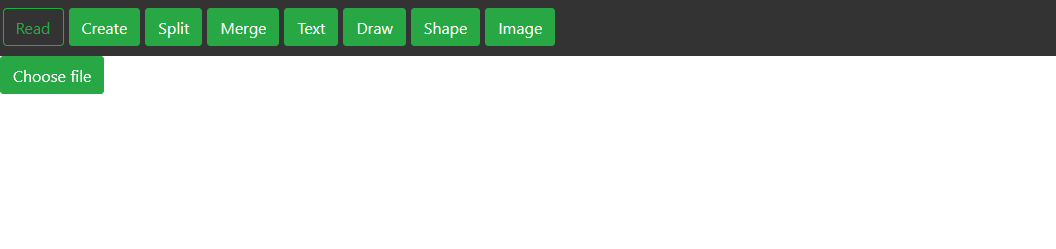
\includegraphics[width=1\textwidth]{"images/startseite.png"}
	\caption{Startseite der PDF Web App}
	\label{fig:start}
\end{figure}

Alle Module unterstützen Input und Output PDFs von maximal 5000 Seiten. Bei fast allen Modulen gibt es Möglichkeiten Benutzereingaben zu machen. Die Benutzereingaben sind so umgesetzt, dass sie bei ungültigem Input automatische korrigiert werden oder die darauf bezogene Operation nicht ausgeführt wird. Gibt man in ein input field, wo eine Zahl erwartet wird, einen String ein, so wird dessen Funktion nicht angewendet. Liegt eine Benutzereingabe als Zahl unter oder über dem minimalen oder maximalen Schwellenwert des Eingabefeldes, so wird die Eingabe mit dem niedrigsten oder obersten Wert substituiert. Manche Eingabefelder erwarten Integers, anstatt Floats, z.B. das Eingabefeld für die Seitenzahl. In diesem Fall wird die Nachkommastelle automatisch von der Benutzereingabe entfernt. Haben sich beim Benutzer ein oder mehrere Leerzeichen in die Eingabe eingeschlichen, so werden diese Leerzeichen von der Anwendung automatisiert erkannt und entfernt. Falls eine andere Dateiart als .pdf unabhängig vom Modul der App geöffnet wurde, erscheint die Fehlermeldung in Screenshot \ref{fig:errorfile}. 

\begin{figure}[!htbp]
	\centering
	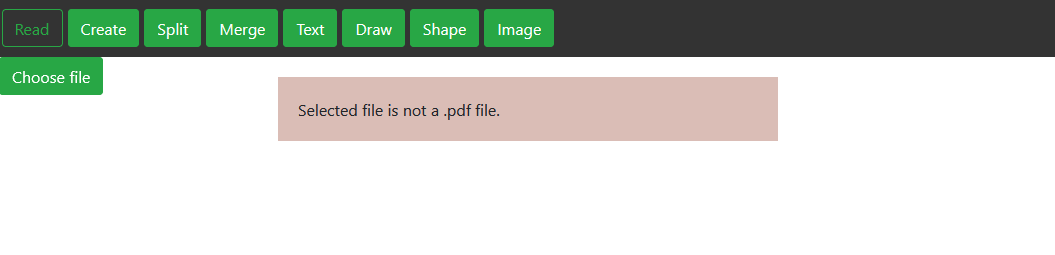
\includegraphics[width=1\textwidth]{"images/errorfile.png"}
	\caption{Fehlermeldung bei einer nicht-PDF-Datei}
	\label{fig:errorfile}
\end{figure}

Auch beim Versuch eine verschlüsselte PDF-Datei zu öffnen, wird eine in Screenshot \ref{fig:errorcrypt} dargestellte Fehlermeldung angezeigt.

\begin{figure}[!htbp]
	\centering
	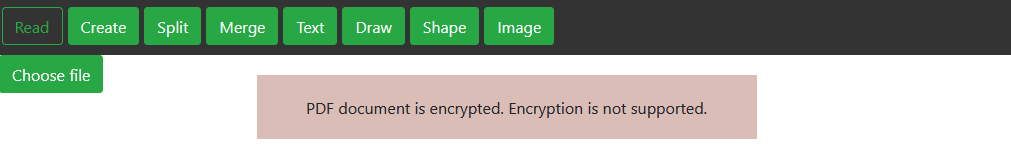
\includegraphics[width=1\textwidth]{"images/errorcrypt.png"}
	\caption{Fehlermeldung bei einem verschlüsselten PDF}
	\label{fig:errorcrypt}
\end{figure}

Bei diesen gezeigten Fehlermeldungen kann man erneut den Dateibrowser im jeweiligen Modul öffnen und eine unverschlüsselte PDF-Datei auswählen oder einen anderen Hauptmenüpunkt wählen, damit die Fehlermeldung verschwindet. \\
Ist ein Modul der PDF Web App geöffnet, so wird der entsprechende Hauptmenübutton durch einen dunkelgrauen Hintergrund mit grüner Schrift symbolisiert. Initial ist der Reader ausgewählt. Der Button Create führt zum Creator für leere PDFs, Split zum Splitter für das Seiten Zerteilen, Merge zum Merger für das Zusammenfügen von PDF-Dateien, Text zum Writer für Textbearbeitung, Draw zum Drawer fürs Zeichnen, Shape zum Geometry Editor zur Geometrieerstellung und Image zum Image Editor zur Bildbearbeitung. Befindet man sich im Reader, Merger, Splitter oder Creator und klickt dann auf ein Editormodul, so wird standardmäßig der Texteditor ausgewählt. Man muss dann nochmals auf ein anderes Editormodul klicken, um es auszuwählen. Jedes Modul der PDF Web App hat einen grünen Save Button, mit dem der Benutzer das editierte PDF als ZIP-Archiv downloaden kann. Es wird im Downloads-Ordner im lokalen Dateisystem abgelegt. Bewegt man die Maus über den Save Button erscheint eine schwarze Dialogbox, in der man einen benutzerdefinierten Dateinamen vergeben kann. Hat man einen benutzerdefinierten Dateinamen eingegeben, so erhält das Output-PDF und der ZIP-Ordner diesen Namen, ansonsten wird ein default Namen verwendet, der aus dem Ursprungsdateinamen und einem Suffix besteht. Der Screenshot \ref{fig:save} bildet die Dialogbox zur Vergabe des Dateinamens ab. 

\begin{figure}[!htbp]
	\centering
	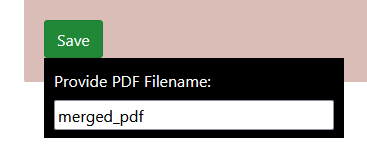
\includegraphics[width=0.6\textwidth]{"images/save.png"}
	\caption{Dateibenennungsdialog des Save Buttons der PDF Web App}
	\label{fig:save}
\end{figure}

Bei Read, Text, Draw, Shape und Image erscheint zunächst der Choose file Button, damit man im Dateisystem ein PDF-Dokument auswählen kann zum Lesen oder Bearbeiten. Klickt man auf Choose file wird der Dateibrowser geöffnet und man kann ein einzelnes PDF zum Öffnen auswählen. Ein geöffnetes Dokument passt seine Zoomgröße automatisch an das Browserfenster an, falls es bei 100 \% über das Browserfenster hinausragen würde, sodass es fast formatfüllend mit etwas Abstsand zum Rand in den Viewport des Browserfensters passt. 

\subsection{Bedienung des Readers}
Der Reader mit geöffneter PDF-Datei präsentiert sich in Screenshot \ref{fig:reader}.

\begin{figure}[!htbp]
	\centering
	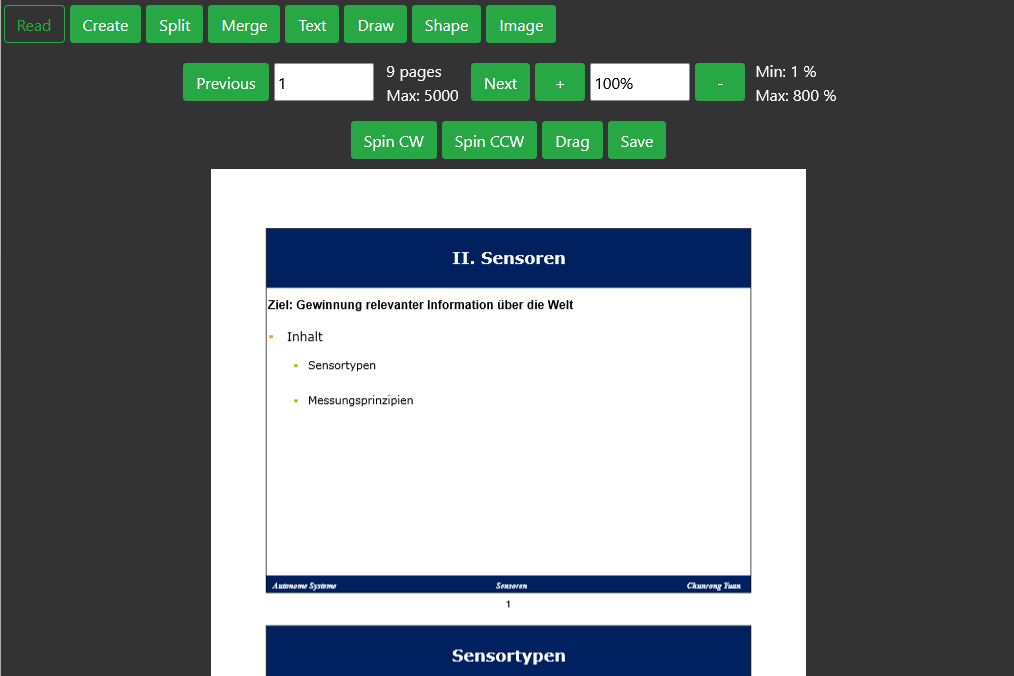
\includegraphics[width=1\textwidth]{"images/reader.png"}
	\caption{Geöffnetes PDF im Reader der PDF Web App}
	\label{fig:reader}
\end{figure}

Hat der Anwender eine PDF-Datei im Reader geöffnet, so entdeckt er 2 dunkelgraue Leisten mit Funktionsbuttons. Mittels Previous und Next kann der Benutzer zur vorherigen bzw. nächsten Seite blättern. Zwischen diesen Buttons informiert das page counter input field über die aktuelle Seite im Viewport und rechts daneben ist die Anzahl an Seiten im Dokument zu sehen. Im page counter input field kann man eine Seitenzahl des Dokuments eingeben, mit Enter bestätigen und der Reader springt direkt zu dieser Zielseite. Alternativ kann man mit dem Scrollbar am linken Browserfensterrand oder dem Scrollrad der Maus durch die Seiten scrollen. Mittels der Buttons Plus und Minus kann man in 20 \%-Schritten rein- bzw. rauszoomen. Der aktuelle Zoomwert in Prozent wird im input field dazwischen signalisiert. Der Anwender kann den Zoomwert auch auf einen gewünschten Wert mit oder ohne Prozentzeichen setzen und Enter drücken, damit der Zoomwert angewendet wird. Wird kein Prozentzeichen über die Tastatur eingegeben, sondern nur der Wert, so wird ein Prozentzeichen von der Anwendung hinzugefügt. Dabei werden nur ganze Zahlen ohne Nachkommastellen berücksichtigt. Außerdem wird der minimale und maximale Zoomwert in Prozent angezeigt. Spin CW und Spin CCW dreht die aktuelle Seite, die im page counter steht, um 90 Grad-Intervalle im Uhrzeigersinn (clockwise) und gegen den Uhrzeigersinn (counterclockwise). Durch den Button Drag kann man die aktuelle Seite im Viewport verschieben. Das ist beispielsweise nützlich, wenn man an das PDF besonders nah rangezoomt hat und die Seite nur teilweise sehen kann, weil man einen kleinen Laptopbildschirm besitzt. Dabei klickt man zuerst auf Drag, hält die Maustaste auf der aktuellen Seite gedrückt und bewegt sie in die gewünschte Richtung. Dabei verschiebt sich nicht nur die aktuelle Seite, sondern alle Seiten und der Mauscursor wechselt das Aussehen zu einem weißen Kreuz mit Pfeilen an den Enden.

\subsection{Bedienung des Creators}
Der Creator ist mittels des Create Buttons im Hauptmenü aufrufbar. Im Screenshot \ref{fig:creator} ist die GUI vom Creator dargestellt. 

\begin{figure}[!htbp]
	\centering
	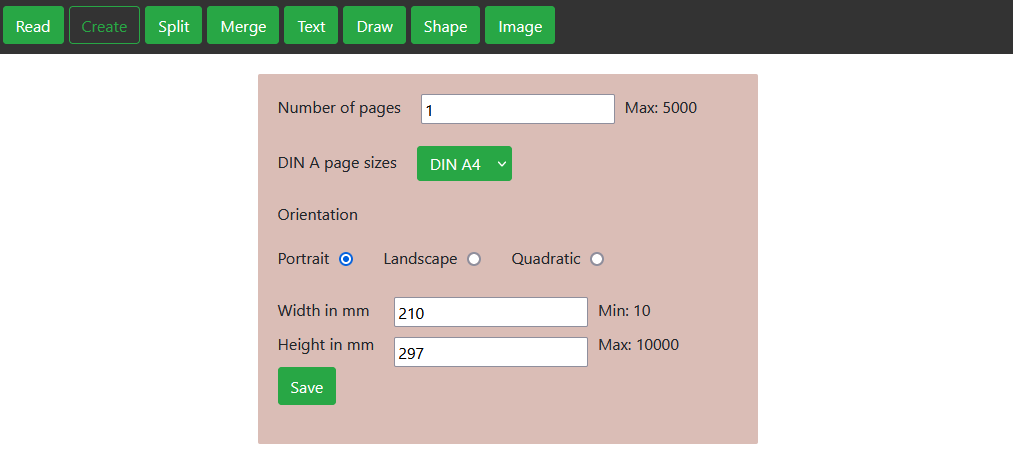
\includegraphics[width=1\textwidth]{"images/creator.png"}
	\caption{Creator GUI der PDF Web App}
	\label{fig:creator}
\end{figure}

Man gibt eine Anzahl an gewünschten Seiten des leeren PDFs ein, sowie die Breite und Höhe in mm. Wahlweise kann man den Selector benutzen, um ein DIN A-Preset zu verwenden. Mittels der Schnellauswahl kann man die Orientierung bestimmten: Portrait, Landscape oder Quadratisch. Minimale und maximale Werte für die Anzahl an Seiten und die Breite und Höhe sind ebenfalls abgebildet. 


\subsection{Bedienung des Splitters}
Zum Splitter kann man mit dem Split Button gelangen, dessen GUI vom Screenshot \ref{fig:splitter} gezeigt wird.

\begin{figure}[!htbp]
	\centering
	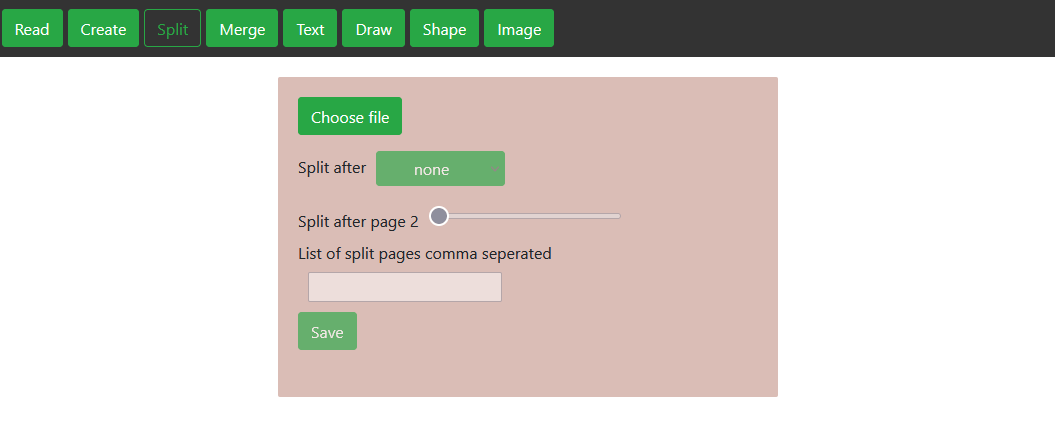
\includegraphics[width=1\textwidth]{"images/splitter.png"}
	\caption{Splitter GUI der PDF Web App}
	\label{fig:splitter}
\end{figure}

\begin{figure}[!htbp]
	\centering
	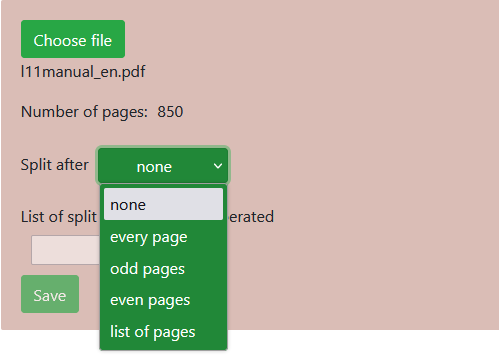
\includegraphics[width=0.7\textwidth]{"images/splitter2.png"}
	\caption{Splitter Selector der PDF Web App}
	\label{fig:splitter2}
\end{figure}

Hat man eine Datei ausgewählt, so wird der Dateiname und die Anzahl an Seiten des Dokuments angezeigt. Durch erneutes Klicken des Choose file Buttons öffnet sich erneut der Dateidialog und man kann ein anderes PDF auswählen. Dabei ersetzt das neue PDF das vorherige, denn man kann nicht mehrere PDF-Dateien gleichzeitig splitten. Im Auswahlmenü kann man zwischen Zerteilen nach jeder, jeder geraden, jeder ungeraden und einer Liste von Seiten auswählen, was in Abbildung \ref{fig:splitter2} dargestellt ist. Wählt man list of pages aus, so kann man die einzelnen Seitennummern mit Komma separiert oder auch nur eine einzelne Seitennummer eintippen. Die Seitenzahlen müssen nicht in aufsteigender Reihenfolge angegeben werden. Bei ungültigen Eingaben wird das Eingabefeld für die Seitenzahlen automatisch gelöscht. 

\subsection{Bedienung des Mergers}
Der Merger ist mit dem Hauptmenüpunkt Merge zu öffnen. Abbildung \ref{fig:merger} zeigt die Startseite des Mergers. 

\begin{figure}[!htbp]
	\centering
	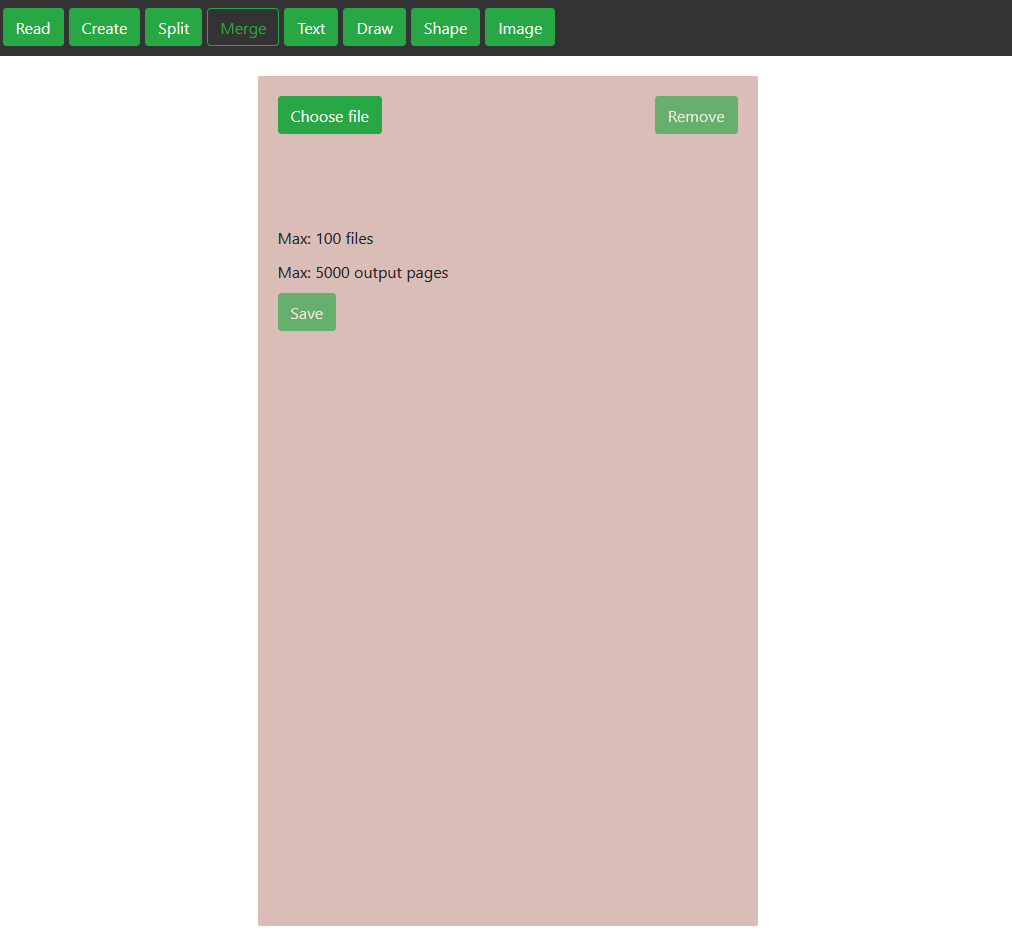
\includegraphics[width=1\textwidth]{"images/merger.png"}
	\caption{Merger Startseite der PDF Web App}
	\label{fig:merger}
\end{figure}

Hier kann man nacheinander mehrere Dateien mittels Choose file öffnen und sie erscheinen je nach Auswahlreihenfolge untereinander in einer scrollbaren Liste, wobei die zuerst ausgewählte Datei am Anfang der Liste steht. In der Liste kann man dann eine Quelldatei mit gedrückter Maustaste zu einer Zieldatei in der Liste ziehen. Lässt man die Maustaste los, so wird die mit der Maus bewegte Datei in diese Listenposition eingefügt. Man kann außerdem eine Datei in der Liste selektieren und mittels des Remove Buttons wieder aus der Liste entfernen. Eine selektierte Datei wird durch einen schwarzen Hintergrund, was der Screenshot \ref{fig:mergelist} verdeutlicht, symbolisiert.

\begin{figure}[!htbp]
	\centering
	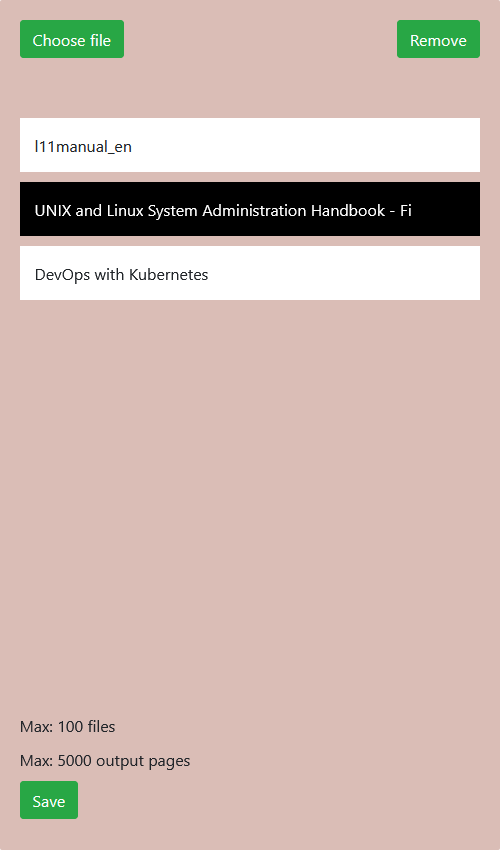
\includegraphics[width=0.8\textwidth]{"images/mergelist.png"}
	\caption{Merger Dateiliste der PDF Web App mit selektierter Datei}
	\label{fig:mergelist}
\end{figure}

Der Benutzer kann zu jeder Zeit erneut den Dateibrowser bedienen, unabhängig davon, ob die Dateiliste bereits modifiziert wurde und der Save Button mergt alle PDF-Dateien in der gegenwärtigen Liste mit der obersten Datei zuerst und der letzten am Schluss des Output PDFs.

\subsection{Bedienung des Editors}
Der Editor ist über den Text-, Draw-, Shape- oder Image-Button erreichbar. Ebenso wie im Reader erscheint zuerst ein Button Choose file. Je nachdem ob nach erstmaligem Öffnen einer PDF-Datei auf Text, Draw, Shape oder Image geklickt wurde, wird als erstes der Writer-, Drawer-, Shaper- oder Imager-Bearbeitungsmodus geöffnet. Ist eine Datei geöffnet, so ist der Reader, ohne die Operationen zum Seiten Drehen, Teil jedes Editormoduls. Alle input fields im Editor sind mit dem gültigen Wertebereich für Benutzereingaben als Information Min: Max: versehen. Der Editor samt dargestellter PDF-Datei besteht aus einem grauen, waagerechten Operations Bar, einem linken Layers Seitenmenü in Rosa und einem rechten grünen Tools Seitenmenü. Mit dem ganz linken, grünen Button Layers im Operations Bar kann das Layers Seitenmenü aus- und eingeblendet werden. Daneben zeigt oder verbirgt der Button Tools das Tools Seitenmenü. Standardmäßig sind Layers und Tools ausgeklappt. Beim Öffnen einer PDF-Datei, wird eine Infobox, die über den Fortschritt der gerenderten PDF-Seiten informiert, angezeigt. Ebenso wird eine Infobox angezeigt, die Auskunft darüber gibt, dass gerade der Speicherprozess in Gange ist. Hat man Text, Drawings, Shapes oder Images hinzugefügt und klickt auf Save, so wird das PDF zuerst auf 500 \% gezoomt, damit die Elemente als Bilder in hochwertiger Qualität eingebettet werden können. Am Ende des Speichervorgangs wird wieder auf den aktuellen Zoomwert des Benutzers zurück gezoomt. Diese beiden Infoboxen, die in Screenshot \ref{fig:render-info} und \ref{fig:save-info} abgebildet sind, sind auch im Reader vorhanden. Die einzelnen Speicherschritte werden in der Webkonsole der Web Developer Tools des Browsers ausgegeben, was in Bild \ref{fig:save-progress-steps} zu sehen ist.

\begin{figure}[!htbp]
	\centering
	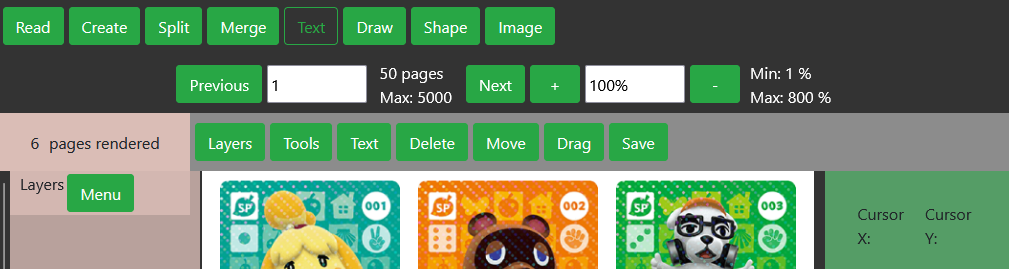
\includegraphics[width=1\textwidth]{"images/render-info.png"}
	\caption{Infobox über den Renderfortschritt der PDF Web App}
	\label{fig:render-info}
\end{figure}

\begin{figure}[!htbp]
	\centering
	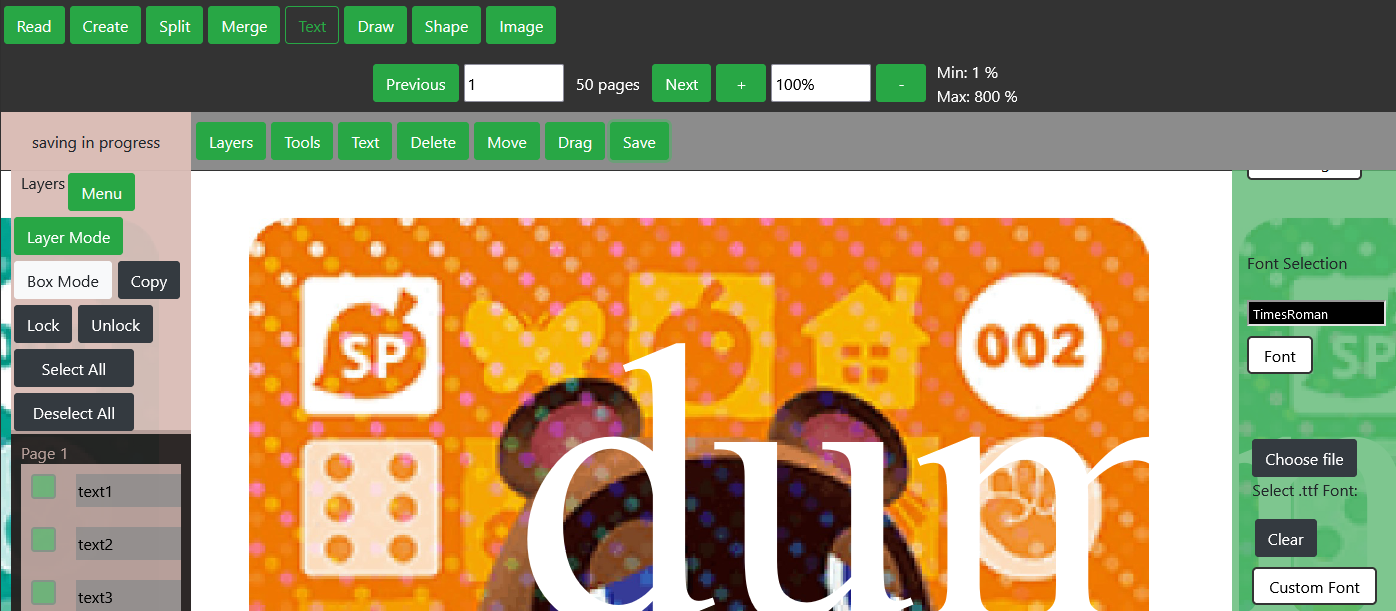
\includegraphics[width=1\textwidth]{"images/save-info.png"}
	\caption{Infobox über den Speicherprozess der PDF Web App}
	\label{fig:save-info}
\end{figure}

\begin{figure}[!htbp]
	\centering
	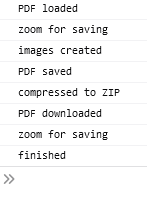
\includegraphics[width=0.4\textwidth]{"images/save-progress-steps.png"}
	\caption{Speicherschritte der PDF Web App in der Webkonsole beim Speichern von Elementen}
	\label{fig:save-progress-steps}
\end{figure}

\subsubsection{Textbearbeitung}
Hat man den Writer aufgerufen, so präsentiert sich einem der Texteditor in den folgenden Abbildungen \ref{fig:texteditor} und \ref{fig:texteditor2}.

\begin{figure}[!htbp]
	\centering
	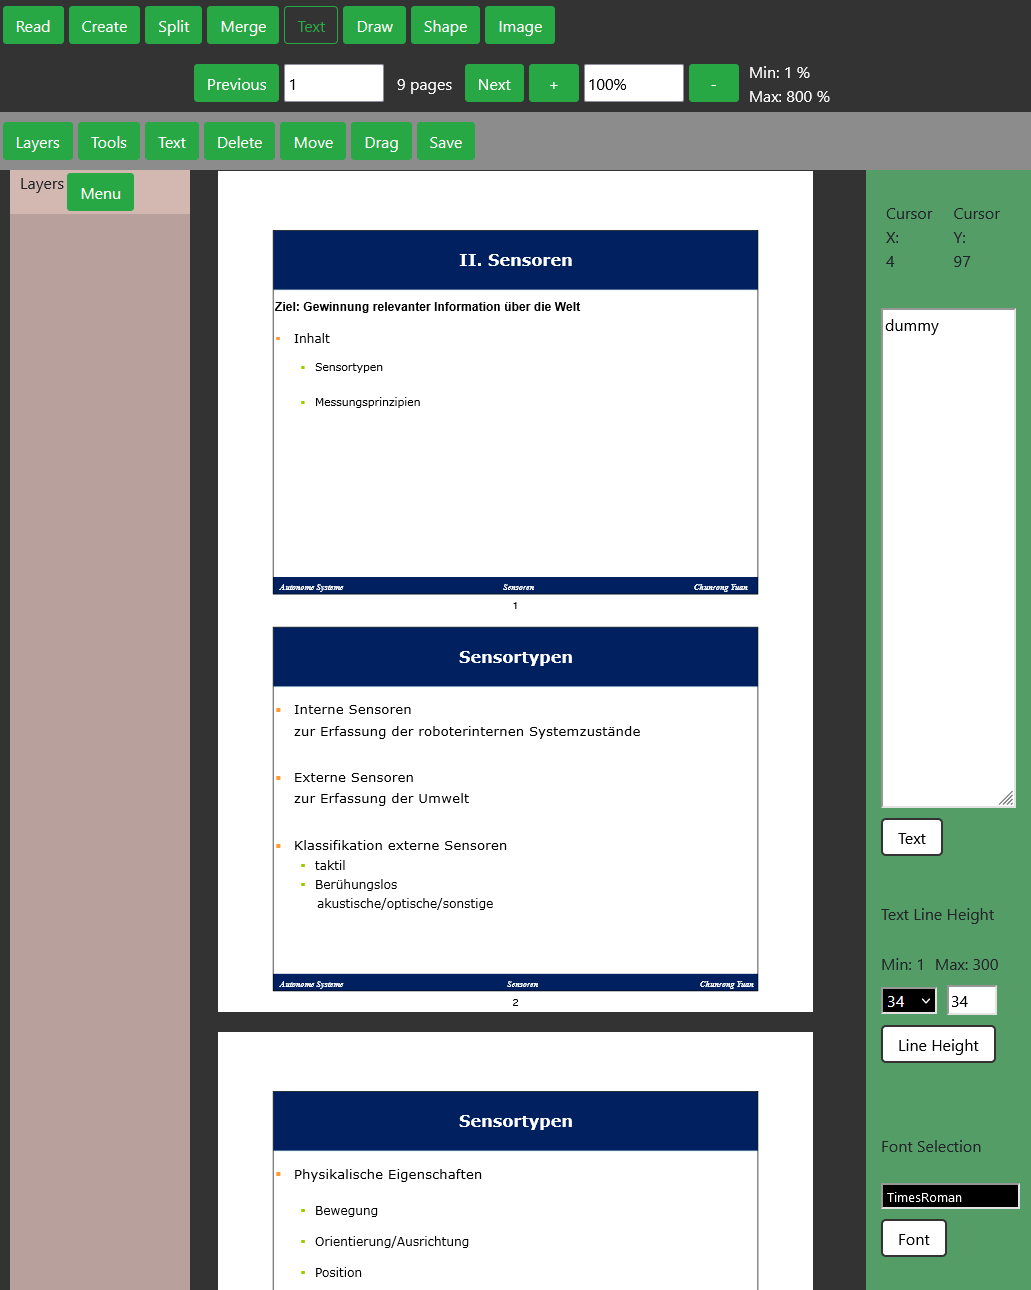
\includegraphics[width=1\textwidth]{"images/texteditor.png"}
	\caption{Startseite des Writers der PDF Web App}
	\label{fig:texteditor}
\end{figure}

\begin{figure}[!htbp]
	\centering
	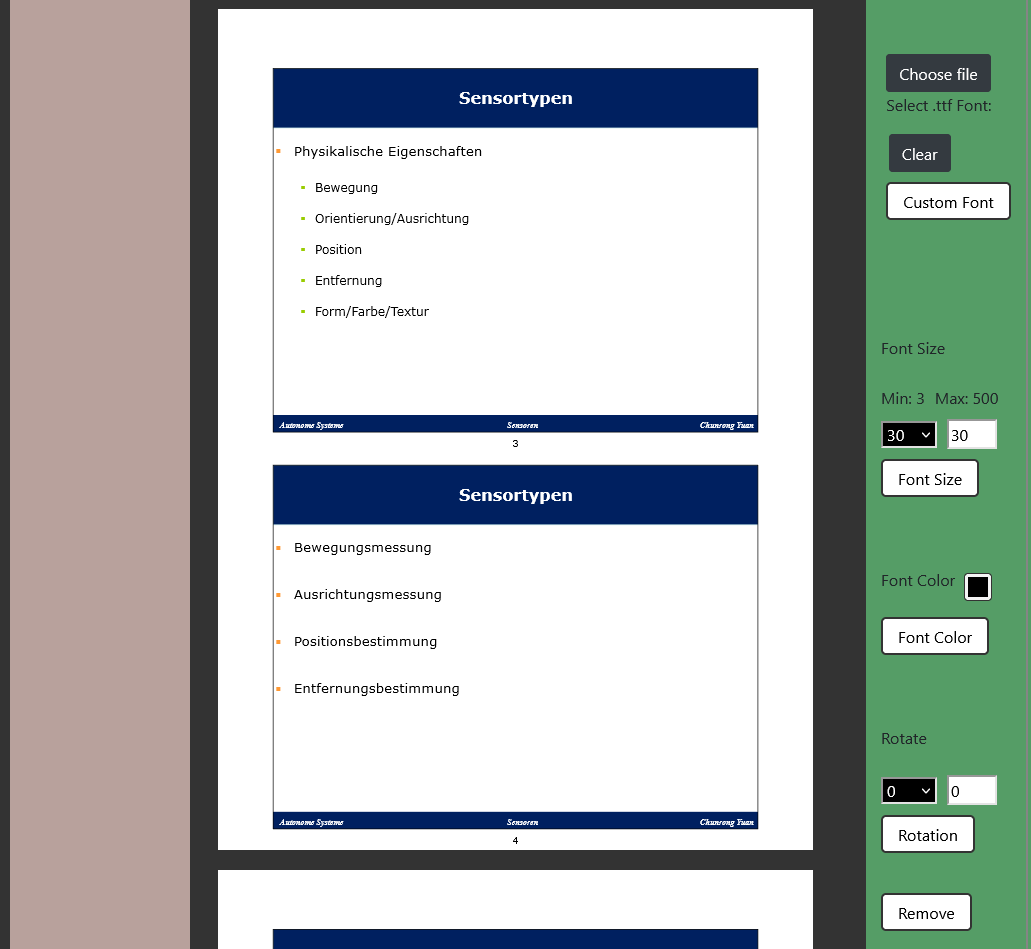
\includegraphics[width=1\textwidth]{"images/texteditor2.png"}
	\caption{Mehr Tools der Startseite des Writers der PDF Web App}
	\label{fig:texteditor2}
\end{figure}

Mit dem Button Text im Operations Bar und nachfolgendem Klick auf das geöffnete Dokument, wird der Platzhaltertext dummy hinzugefügt. Unter dem Text erscheint eine dunkelrote controlBox, auf die man alle Operationen im Operations Bar und in Tools im Box Mode anwenden kann. Ich werde zunächst alle Operationen im Box Mode beschreiben und später auf den Layer Mode eingehen. Der Box Mode ist standardmäßig eingestellt. Operationen können durch die grünen Buttons zum Erstellen neuer Elemente, Delete und Move im Operations Bar und allen weißen Buttons in Tools getriggert werden. Hat man eine Operation getriggert, so befindet man sich im Modus dieser Operation im Box Mode. Darauffolgend können alle, im Dokument verfügbaren controBoxes angeklickt werden, um die Operation auf das betreffende Element auszuführen. Alle Operationen in Tools beziehen sich jeweils auf das Element des aktuellen Editormoduls und sind nur auf diesem anwendbar. Versucht man eine Operation eines Editormoduls auf ein Element eines anderes Editormoduls anzuwenden, wird die Operation nicht ausgeführt. In der Praxis des Box Modes kann man mehrere Texte, ohne erneut den grünen Text Button drücken zu müssen, dem PDF-Dokument hinzufügen. Für jedes neu hinzugefügte Editorelement wird eine Layer, mit einem elementspezifischen Standardnamen erstellt, die in Layers erscheint. Die obere linke Ecke der quadratischen controlBox von sämtlichen Editorelementen wird an der Stelle platziert, an der man mit der Maus auf die Seite geklickt hat. Alle controlBoxes werden nicht im  Output-PDF gespeichert, denn sie dienen lediglich der Steuerung von Editorelementen, um Operationen im Box Mode anwenden zu können. Mit dem Delete-Button und nachfolgendem Klick in eine oder mehrere controlBoxes im Box Mode, können Texte wieder gelöscht werden. Move verschiebt einzelne Texte durch eine mit der Maus gedrückten und zur Zielposition bewegten controlBox. Sobald die Maus losgelassen wird, nachdem die controlBox verschoben wurde, springt der Text an die Zielposition auf der Seite. Dabei ist wichtig zu beachten, dass man die controlBox langsam verschiebt, denn der Mauszeiger muss innerhalb der controlBox bleiben. Delete und Move kommen in allen Editormodulen vor und funktionieren immer gleich. Ganz oben in Tools werden dem Betrachter die x- und y-Koordinaten des Mauscursors auf der PDF-Seite angezeigt, während die Maus über eine Seite bewegt wird. Diese Mauscursorkoordinaten sind in jedem Editormodul präsent. Textelemente lassen sich in der textarea editieren. Zeilenumbrüche werden berücksichtig. Nachdem der dummy Text in der textarea überschrieben wurde, ein Klick auf den weißen Text-Button erfolgte und die Operation auf eine controlBox angewendet wurde, substituiert sich der Platzhaltertext mit dem aktuellen Text in der textarea. Die textarea kann in vertikaler Höhe expandiert werden. In allen Editormodulen von Tools werden alle Operationen exakt gleich ausgeführt: Man tätigt seine Einstellung, drückt mit der linken Maustaste auf den weißen Button für die jeweilige Operation und klickt daraufhin auf eine oder mehrere controlBoxes von Elementen. Unterhalb der Texteditierungsoperation kann der Zeilenabstand einstellt werden. Entweder verwendet man das selection menu mit voreingestellten Werten oder man gibt einen gewünschten Wert manuell in das input field ein. Neu hinzugefügte Elemente sind standardmäßig vorkonfiguriert. Alle Eingabefelder sämtlicher Editormodule zeigen dessen Standardwerte an. Bei jeder selection menu und input field Kombination ist maßgeblich, welche Schaltfläche zuletzt betätigt wurde. Einen benutzerdefinierten Font als .ttf oder .otf Datei kann man durch den dunkelgrauen Choose file-Button vom Dateisystem auswählen und wird in einer Liste abgebildet. Der zuletzt geöffnete Font wird ausgewählt. Die Selektion des aktuellen Fonts wird durch einen Klick auf den radio button des Fontdateinamens aktiviert. Mittels Clear werden alle Fonts aus der Liste entfernt. Fontdateinamen werden nach 15 Zeichen in die nächste Zeile umgebrochen. Abbildung \ref{fig:custom-font} zeigt 2 geöffnete .ttf Schriftdateien in der Liste.

\begin{figure}[!htbp]
	\centering
	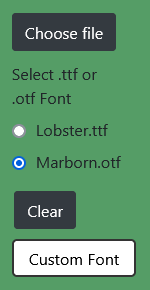
\includegraphics[width=0.2\textwidth]{"images/custom-font.png"}
	\caption{Benutzerdefinierte Fontliste im Texteditor der PDF Web App}
	\label{fig:custom-font}
\end{figure}

Die Fontgröße kann mittels selection menu und input field justiert werden. Bezüglich der Fontfarbe lässt sich ein Color Picker Menü mit Klick auf das initial schwarze Quadrat ausklappen. Es können Farbe und Transparenz eingestellt werden. Die Farbwerte stehen in den Formten RGBA, HSLA oder HEX zur Verfügung. Mit Klick auf die beiden kleinen senkrechten Pfeile im Color Picker wird das Format gewechselt. Das Fenster des Color Pickers für die Fontfarbe ist in Abbildung \ref{fig:fontcolor} dargestellt. 

\begin{figure}[!htbp]
	\centering
	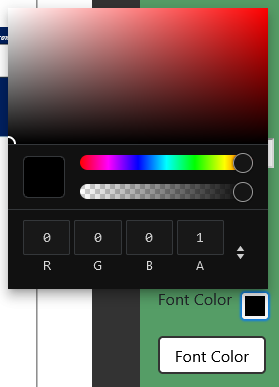
\includegraphics[width=0.5\textwidth]{"images/fontcolor.png"}
	\caption{Color picker für die Fontfarbe des Texteditors der PDF Web App}
	\label{fig:fontcolor}
\end{figure}

Als vorletzte Option kann der Text absolut gedreht werden. Durch den weißen Button Rotation und der entsprechenden Benutzerinteraktion durch selection Menu oder input field wird das Textelement rotiert. Absolute Rotation bedeutet, dass es eine feste Rotationsskala gibt, anhand der das Element rotiert wird. Bei einem Rotationswinkel von 0 Grad ein wird die Ausgangsrotation angewendet. Alle Editormodule arbeiten mit absoluter Rotation. Abschließend können alle Textelemente im Dokument mit dem Remove Button vollständig gelöscht werden. Ein neuer und modifizierter Text wird in Abbildung \ref{fig:text} demonstriert.

\begin{figure}[!htbp]
	\centering
	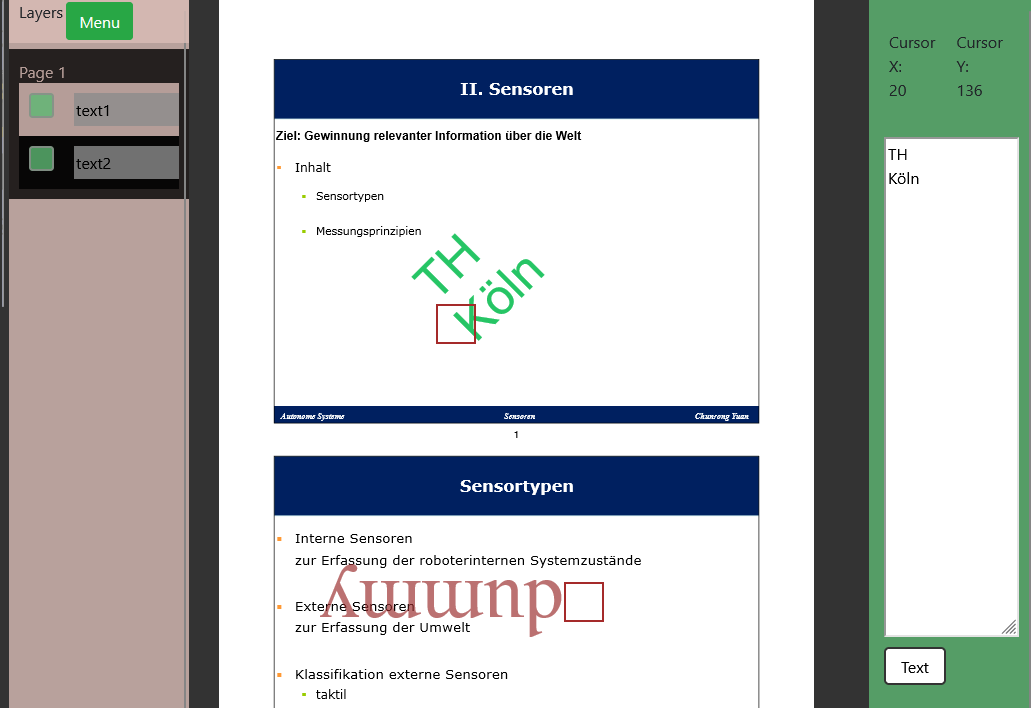
\includegraphics[width=1\textwidth]{"images/text.png"}
	\caption{Bearbeiteter Text im Writer der PDF Web App}
	\label{fig:text}
\end{figure}

\subsubsection{Drawings erstellen}
Der Drawer ist in Screenshot \ref{fig:drawer} abgebildet. 

\begin{figure}[!htbp]
	\centering
	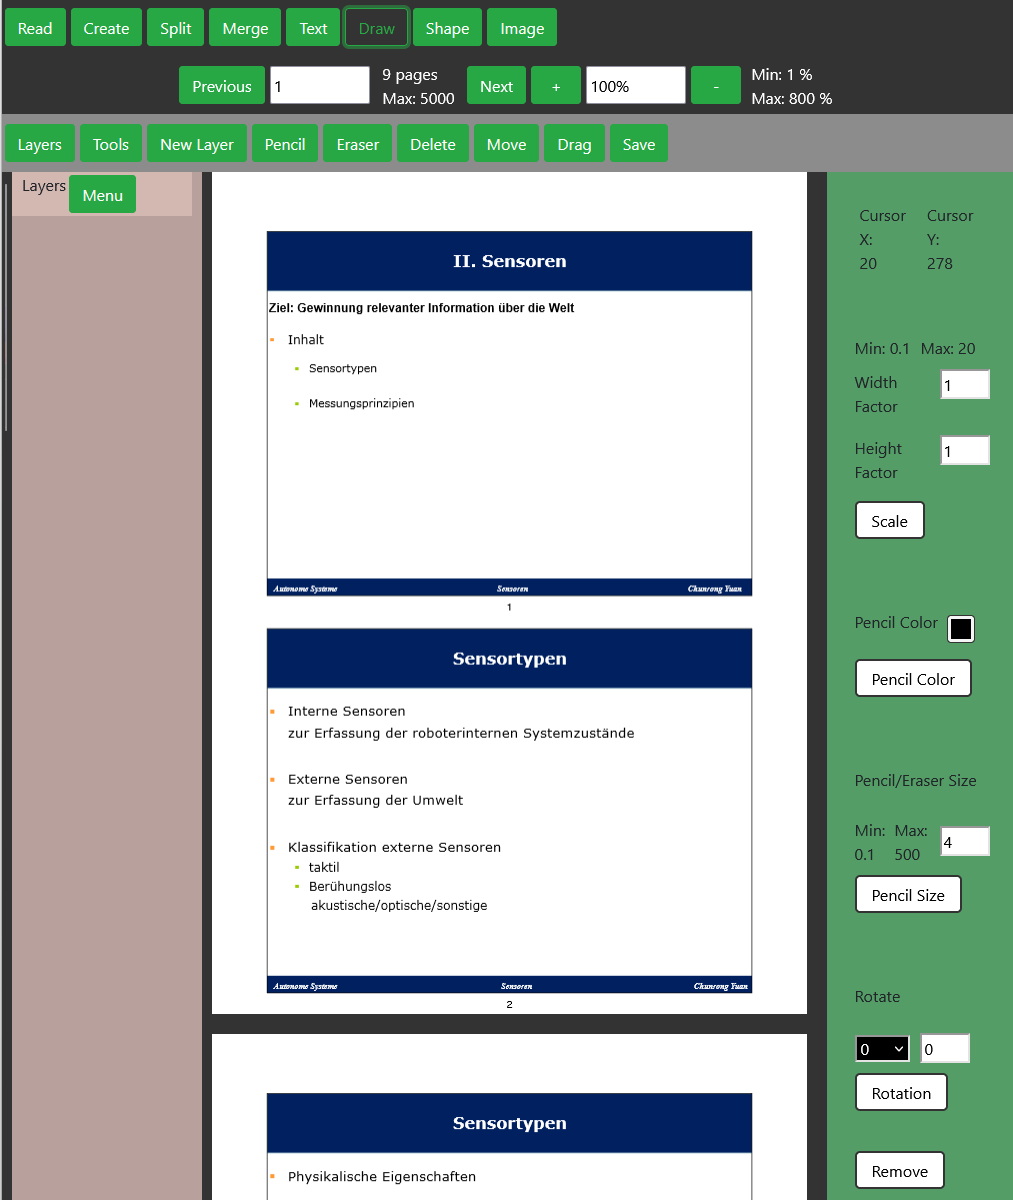
\includegraphics[width=1\textwidth]{"images/drawer.png"}
	\caption{Drawer der PDF Web App}
	\label{fig:drawer}
\end{figure}

Der Zeichenmodus wird mittels Pencil initiiert. Mit gedrückter Maustaste und gleichzeitigen Mausbewegungen erscheint eine Linie. Die Startstelle des Drawings wird durch eine magenta farbige controlBox markiert. Drawings lassen sich idealerweise mit einem Graphic Tablet erstellen. Für das erste Drawing der Seite wird von der Anwendung eine Layer zugewiesen. Mittels des New Layer-Buttons kann eine neue Layer kreiert werden. Falls keine Layer ausgewählt wurde, wird auf der zuletzt gezeichneten Layer der Seite gearbeitet. Generell wird auf der ausgewählten Layer gezeichnet. Der Radierermodus wird durch den Eraser-Button im Operations Bar aktiviert. Mit gedrückter Maustaste können Pixelbereiche des Drawings entfernt werden. Das Drawing zum Radieren wird durch die Auswahl der Layer bestimmt. Das Mauscursorsymbol der Zeichenoperation wird durch ein schwarzes, dünnes Kreuz signalisiert. Im Radierermodus alterniert das Mauscursorsymbol zu einem weißen, dicken Kreuz. Sobald eine Operation in Tools angewendet wird, wird der Zeichenmodus bzw. Radierermodus verlassen. In Tools kann ein Drawing relativ skaliert werden, indem ein Faktor eingegeben wird. Der Faktor kann auch ein Float sein und multipliziert sich immer mit der aktuellen Größe. Im nächsten Bereich definiert ein Color Picker die Stift- und Eraserfarbe inklusive der Deckkraft. Des Weiteren kann der Durchmesser des Stifts bzw. Radierers justiert werden. Ebenfalls können Drawings absolut rotiert werden. Wurde ein Drawing gedreht und auf der Layer weiter gezeichnet, so wird eine weitere Layer von der Anwendung angelegt. In der untersten Sektion von Tools entfernt Remove alle Drawings im Dokument. Teilweise transparente Drawings werden in Abbildung \ref{fig:drawing} dargestellt. 

\begin{figure}[!htbp]
	\centering
	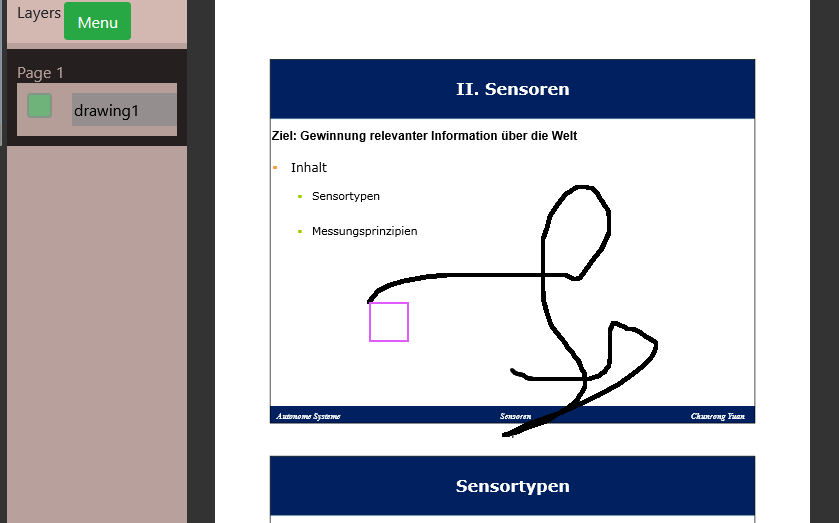
\includegraphics[width=1\textwidth]{"images/drawing.png"}
	\caption{Drawings im Drawer der PDF Web App}
	\label{fig:drawing}
\end{figure}


\subsubsection{Shapes hinzufügen}
Die Startseite des Shapers ist in den Screenshots \ref{fig:shaper} und \ref{fig:shaper2} abgebildet. 

\begin{figure}[!htbp]
	\centering
	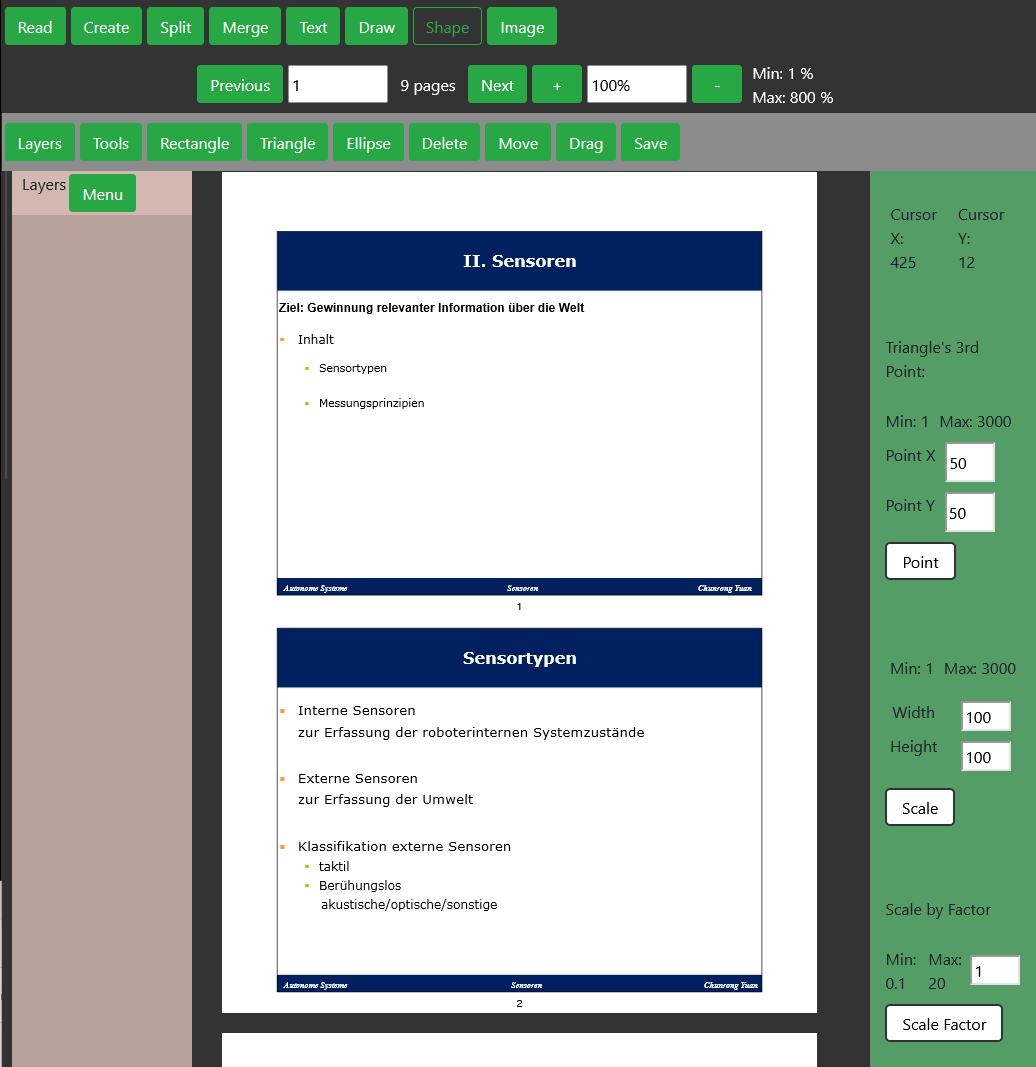
\includegraphics[width=1\textwidth]{"images/shaper.png"}
	\caption{Shaper der PDF Web App}
	\label{fig:shaper}
\end{figure}

\begin{figure}[!htbp]
	\centering
	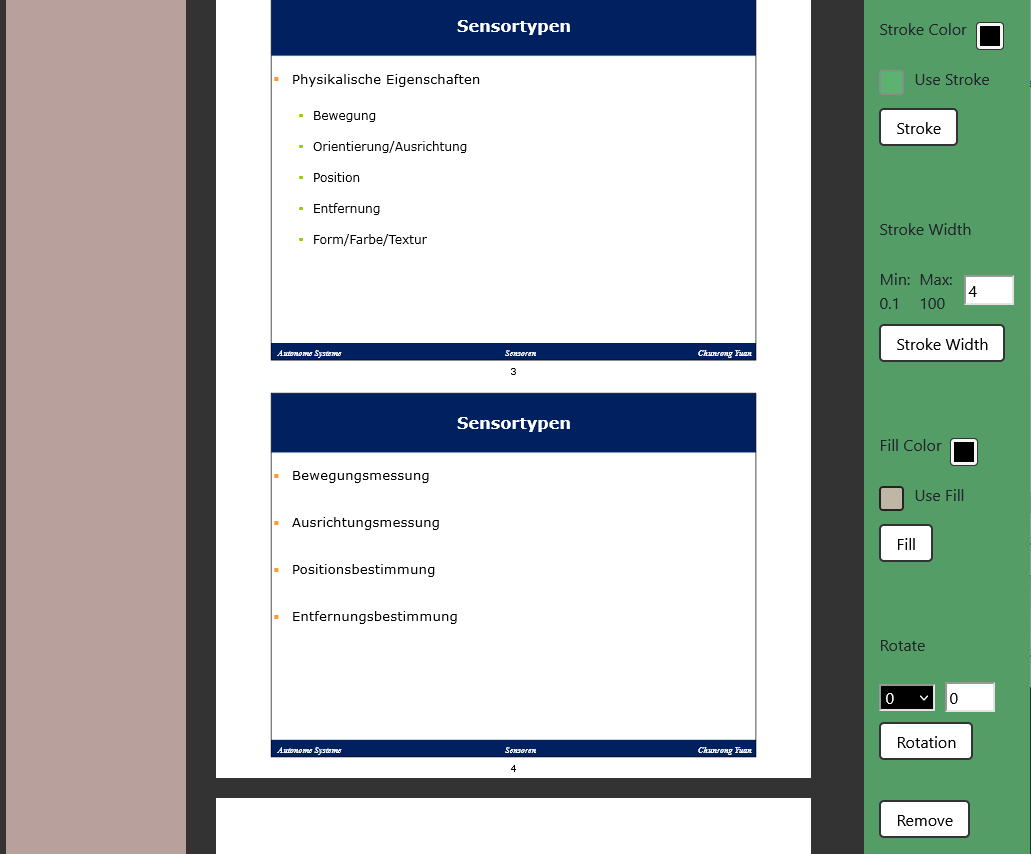
\includegraphics[width=1\textwidth]{"images/shaper2.png"}
	\caption{Mehr Tools des Shapers der PDF Web App}
	\label{fig:shaper2}
\end{figure}

Der Shapetyp kann durch die Buttons Rectangle für Rechteck, Triangle für Dreieck oder Ellipse und einem oder mehreren Klicks auf eine Seite bestimmt werden. Jedem Shape wird eine orange controlBox mehr oder weniger mittig hinzugefügt. In Tools des Shapers gibt es eine einzige Operation, die nur auf Dreiecke angewendet werden kann. Es handelt sich um die oberste Einstellung für die Breite und Höhe des dritten Punktes des Dreiecks (Triangle's Third Point). Mit dieser Operation kann der rechte Punkt der langen Spitze des default Dreiecks bearbeitet werden. Alle anderen Einstellmöglichkeiten können auf sämtlichen Shapeelementen Rectangle, Triangle und Ellipse arbeiten. Die Skalierung von Shapes bietet 2 Vorgehensweisen. Zum einen können Breite und Höhe unabhängig voneinander einstellt werden, was eine absolute Skalierung bedeutet. Zum anderen kann der proportionale, relative Skalierungsfaktor die Größe modulieren. Für die Umrandungslinien des Shapes kann auf der einen Seite die Farbe inklusive Deckkraft und auf der anderen Seite die Breite der Linie justiert werden. Die Strichfarbe muss mit der checkbox Use Stroke in Grün aktiviert sein. Bei Deaktivierung von Use Stroke schaltet sich automatisch die Use Fill checkbox ein und umgekehrt. Beide checkboxes können angehakt (Grün) sein, aber nicht beide zusammen abgehakt (Rosa). Use Fill muss Grün sein, um die Füllfarbe anzuwenden. Bei Strich- und Füllfarbe wird ein Color Picker verwendet. Alle Shapes können mit absoluter Rotation gedreht werden. Die controlBoxes werden durch die Rotation mitgedreht. Zuunterst entfernt der Remove-Button alle Shapes im Dokument. Der Screenshot \ref{fig:shaping} hebt mehrere bearbeitete Shapes hervor.

\begin{figure}[!htbp]
	\centering
	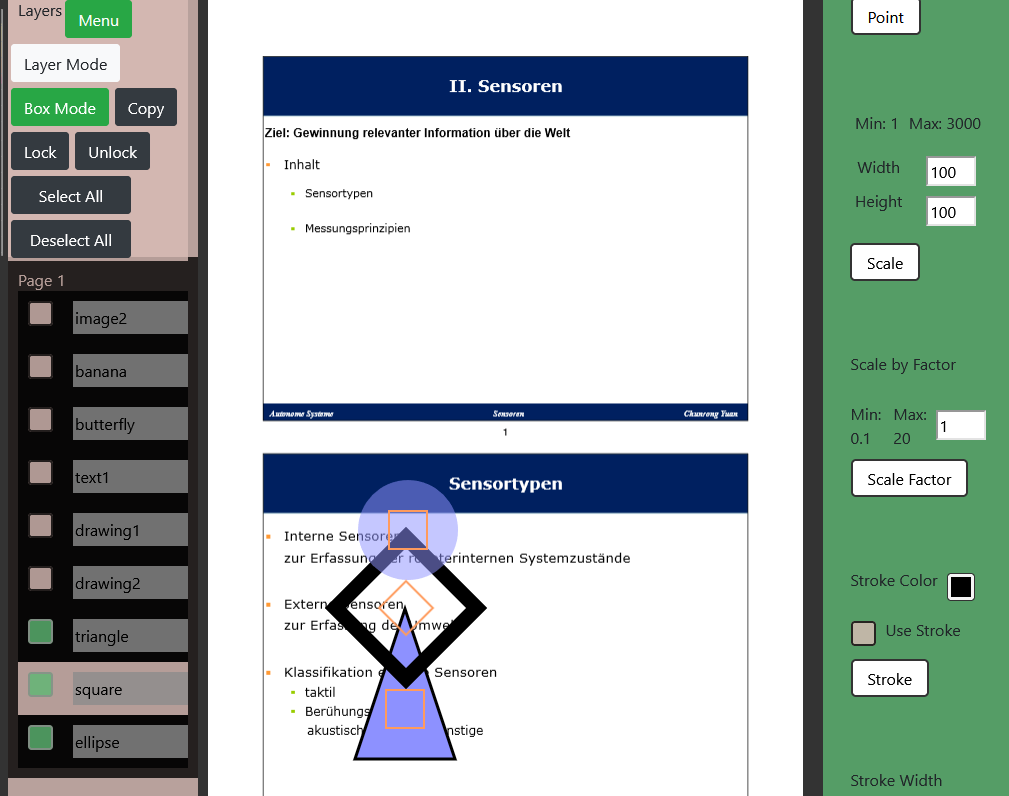
\includegraphics[width=1\textwidth]{"images/shaping.png"}
	\caption{Shapes im Shaper der PDF Web App}
	\label{fig:shaping}
\end{figure}


\subsubsection{Images einfügen}
Der Imager ist in Bild \ref{fig:images} dargestellt. 

\begin{figure}[!htbp]
	\centering
	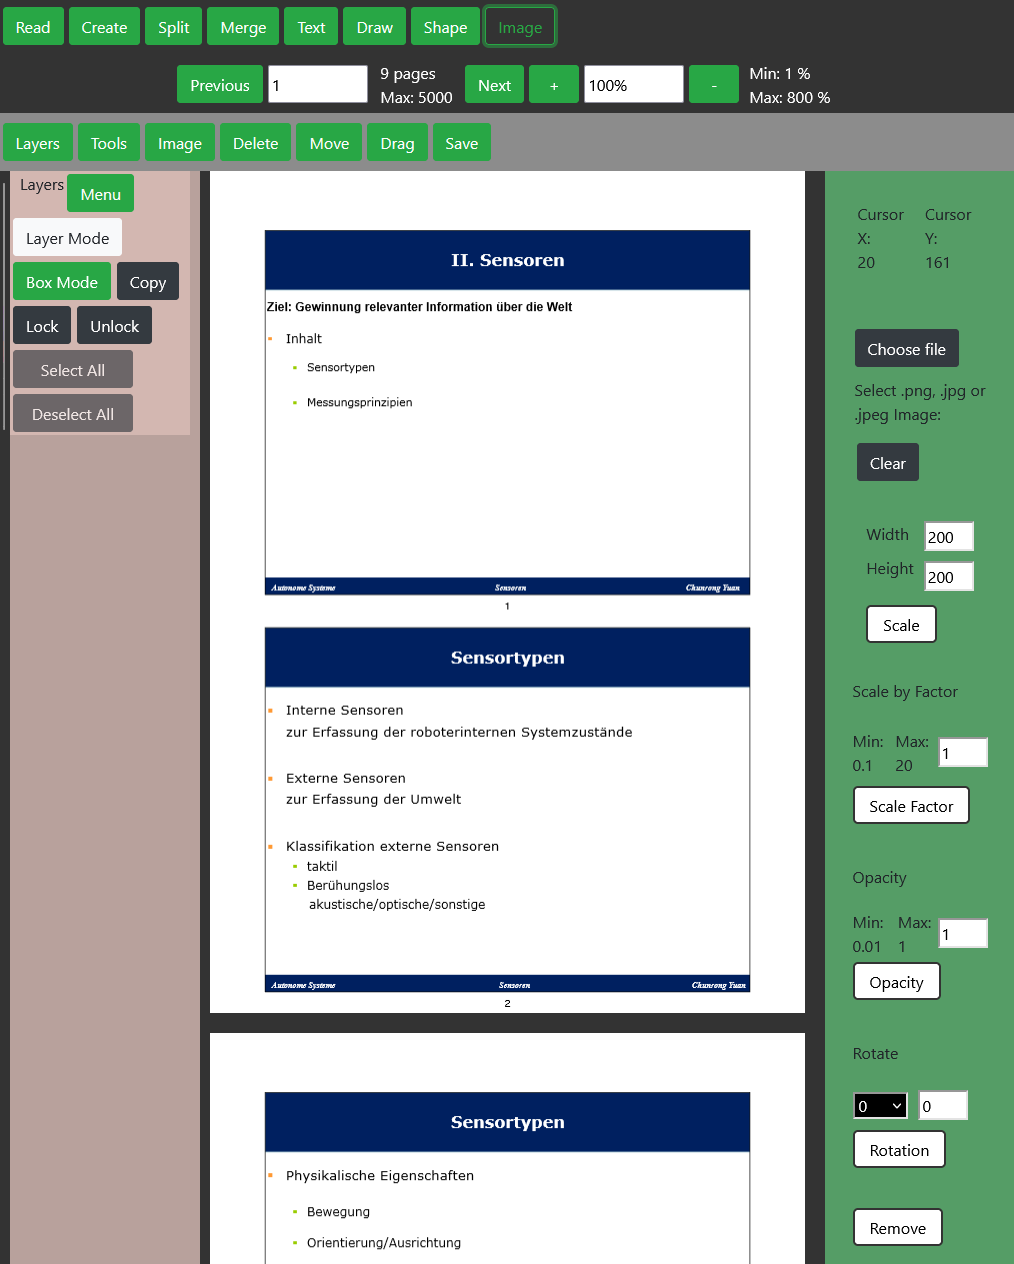
\includegraphics[width=1\textwidth]{"images/images.png"}
	\caption{Imager der PDF Web App}
	\label{fig:images}
\end{figure}

Um ein Image mit dem Image-Button im Operations Bar hinzuzufügen, muss zunächst ein Image mittels des dunkelgrauen Choose file-Buttons im Dateisystem ausgewählt werden. Dadurch erscheint der Imagename in der Liste unter Choose file. Mehrere Images lassen sich nacheinander mittels des Dateidialogs auswählen. Das zuletzt selektierte Image wird automatisch mit einem blauen radio button gekennzeichnet. Zusätzlich werden die Originaldimensionen des Images angezeigt, sobald das Image mittels des grünen Buttons Image im Operations Bar auf der Seite platziert wurde. Eine hellblaue controlBox erscheint bei der Imageplatzierung. Ein Image kann in Breite und Höhe absolut skaliert werden. Auf proportionale Art und Weise wird ein Image mit dem relativen Skalierungsfaktor verkleinert bzw. vergrößert. Unterhalb der Skalierungsoperationen kann die Deckkraft eines Images bestimmt werden. Ebenfalls lässt sich ein Image absolut rotieren. Zuletzt können alle Images im Dokument mit dem Remove-Button entfernt werden. Die Abbildung \ref{fig:imaging} zeigt den Imager in Aktion.

\begin{figure}[!htbp]
	\centering
	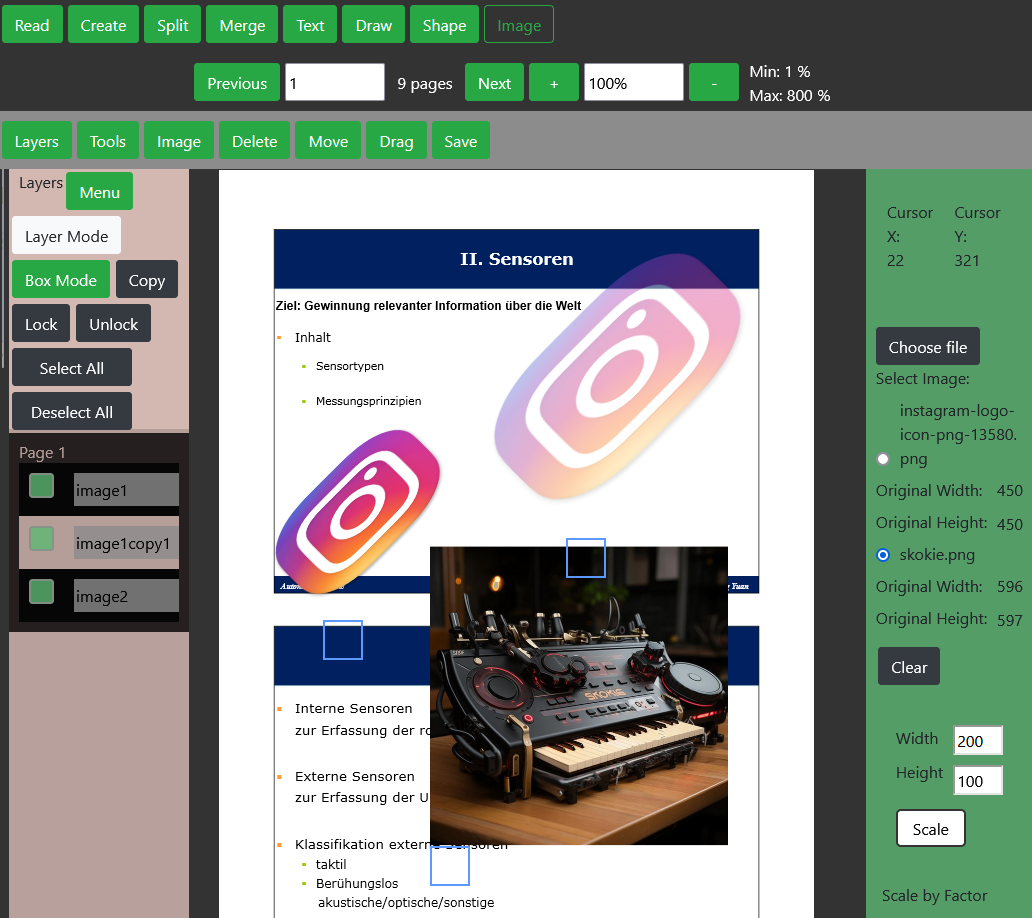
\includegraphics[width=1\textwidth]{"images/imaging.png"}
	\caption{Platzierte Images im Imager der PDF Web App}
	\label{fig:imaging}
\end{figure}

\subsubsection{Ebenensteuerung}
Das in Abbildung \ref{fig:ebenenmenu} gezeigte Layers Menu lässt sich mit einem Klick auf Menu in Layers hervorholen oder verbergen. Es ist möglich durch die Liste an hinzugefügten Layers zu scrollen.

\begin{figure}[!htbp]
	\centering
	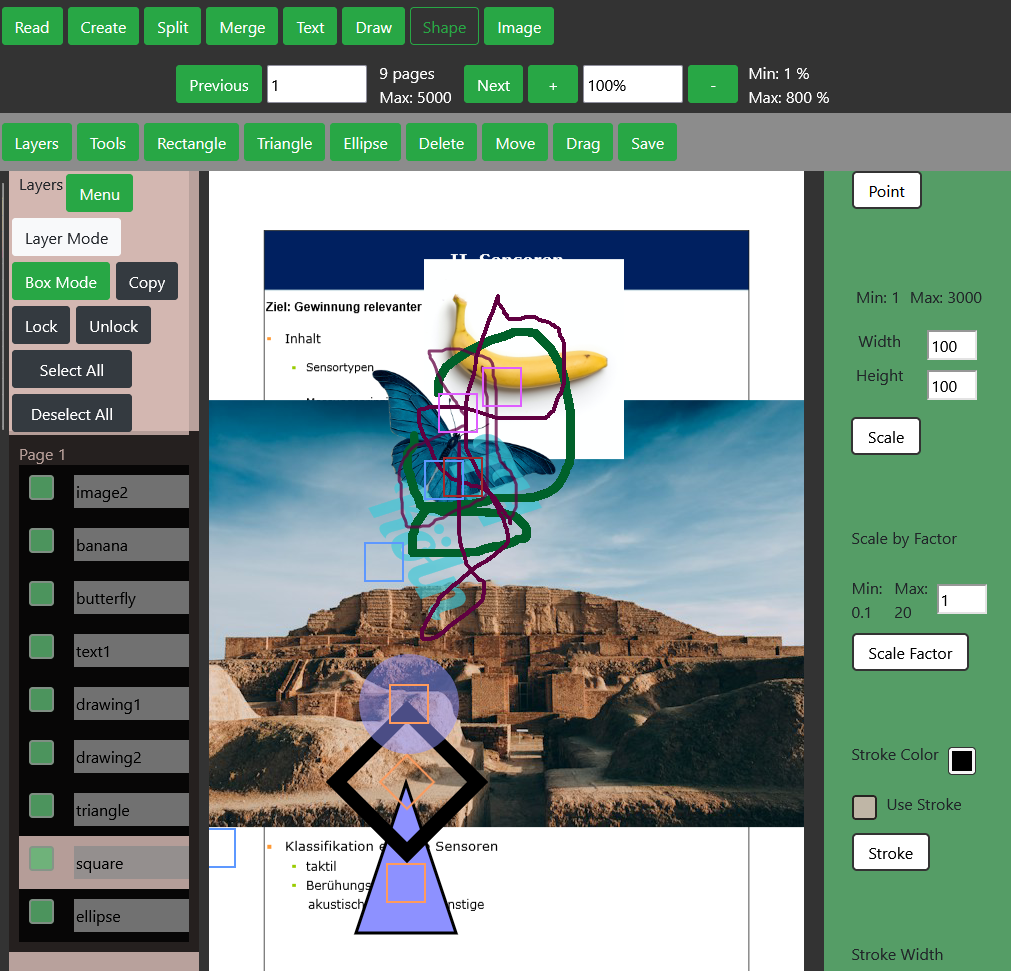
\includegraphics[width=1\textwidth]{"images/ebenenmenu.png"}
	\caption{Ausgeklapptes Layers Menu im Editor der PDF Web App}
	\label{fig:ebenenmenu}
\end{figure}

Standardmäßig sind die Schaltflächen eingeklappt. Fügt man ein Element, unabhängig vom Typ, einer PDF-Seite hinzu, wird für dieses Element eine Layer angelegt, die dann automatisch ausgewählt ist. Layers werden nach aufsteigenden Seitenzahlen gruppiert. Eine ausgewählte Layer ist rosa und eine abgewählte schwarz. Es können mehrere Layers ausgewählt werden. Wenn eine Layer angelegt wird, bekommt sie einen Standardnamen gesetzt, der durch den Elementtyp und einem nummerischen Index, beginnend mit 1, gekennzeichnet ist. Der Standardname kann durch Tastatureingabe im grauen input field auf der Layer überschrieben werden. Layers werden nach Seitenzahlen in einer schwarzen Box, die oberhalb mit der Seitenzahl gekennzeichnet ist, gruppiert. Im Layers Menu kann man zwischen Box Mode und Layer Mode wechseln. Ist der Modus Button grün, so ist der betreffende Modus eingeschaltet. Hingegen ist ein ausgeschalteter Modus mit einem weißen Button versehen. Man kann sich entweder im Box Mode, oder im Layer Mode befinden, aber nicht in beiden Modi gleichzeitig. Mit dem dunkelgrauen Copy-Button kann der Benutzer ausgewählte Layers kopieren. Folglich werden die beinhaltenden Elemente dubliziert. Wird eine Layer kopiert, so wird an den Layernamen copy und eine Nummerierung angehängt. Mit Lock und Unlock kann man Layers sperren bzw. entsperren. Eine locked Layer kann nicht verändert werden, d.h. keine Operationen können auf ihr beinhaltendes Element angewendet werden. Eine locked, unausgewählte Layer ist weiß und eine locked, ausgewählte ist rosa mit weißer Umrandung. 

\begin{figure}[!htbp]
	\centering
	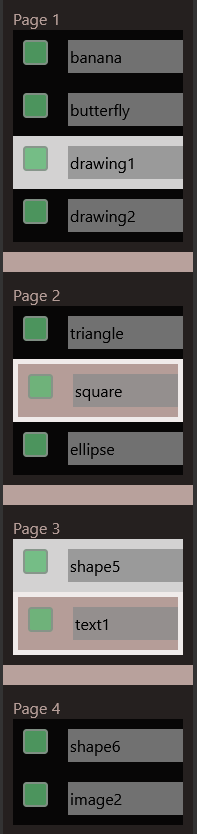
\includegraphics[width=0.3\textwidth]{"images/ebenen.png"}
	\caption{Teilweise locked Layers im Editor der PDF Web App}
	\label{fig:ebenen}
\end{figure}

Die dunkelgrauen Select All und Deselect All Buttons stellen Auswahlfilter dar. Bewegt man die Maus auf die Buttons klappt sich ein Selection Filter Menu auf, was im Bildausschnitt \ref{fig:filtermenu} gezeigt wird. 

\begin{figure}[!htbp]
	\centering
	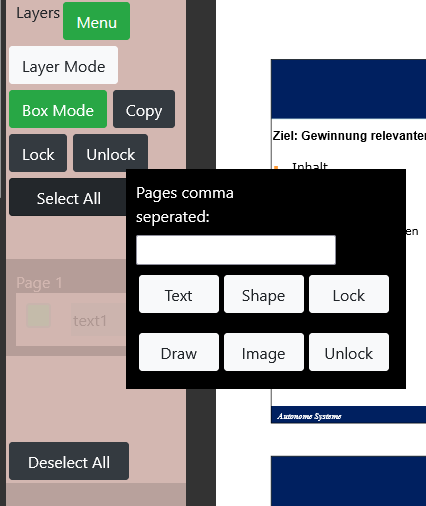
\includegraphics[width=0.6\textwidth]{"images/filtermenu.png"}
	\caption{Selection Filter Menu im Editor der PDF Web App}
	\label{fig:filtermenu}
\end{figure}

Bei Select All kann man mehrere Layers nach Seiten auswählen, nach Elementtyp und, ob sie locked oder unlocked sind, d.h. die Layers werden rosa markiert. Ist ein Selection Filter aktiviert, werden die Buttons im Selection Filter Menu grün. Bei weißen Buttons oder einer leeren Liste an Seiten ist kein Selection Filter aktiviert. Bei der Seitenliste muss man die Seiten durch Komma trennen und sie müssen nicht in aufsteigender Reihenfolge angegeben werden. Die Filter werden mit einem Klick auf Select All angewendet. Ist kein Filter aktiviert, was der Standardzustand ist, so werden alle Layers mit Klick auf Select All ausgewählt. Deselect All hat die gleiche Funktionalität, nur dass die Deselection Filter zum Auswahl aufheben angewendet werden, d.h. Layers werden auf Schwarz gesetzt. Ein Klick auf Deselect All ohne Filter wählt alle Layers im Dokument ab. Im Bildausschnitt \ref{fig:filtering.} ist ein Beispiel von Deselect All Filtern abgebildet. Laut des Beispiels würde die Auswahl auf allen unlocked Textelementen auf Seite 1 und 2 aufgehoben werden. 

\begin{figure}[!htbp]
	\centering
	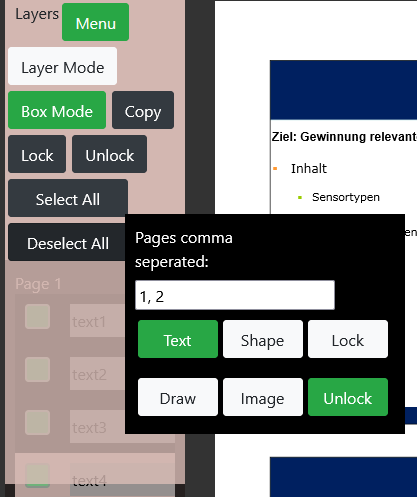
\includegraphics[width=0.6\textwidth]{"images/filtering.png"}
	\caption{Deselection Filter Menu mit aktivierten Filtern im Editor der PDF Web App}
	\label{fig:filtering}
\end{figure}

Sowohl bei Select All als auch bei Deselect All habe ich eine Benutzereingabenkontrolle beim der Seitenlistenfilter implementiert. Falls der Benutzer ungültige Eingaben gemacht hat, z.B. Seiten als Float oder Strings, so wird die Eingabe bei Auslösung des Filters gelöscht. Leerzeichen können zwischen gültigen Seitenzahlen verwendet werden. Folglich wird Select All bzw. Deselect All so angewendet, als ob kein Filter für die Seiten eingestellt wurde, d.h. aktivierte Filter für Elementtypen oder locked bzw. unlocked Layers greifen dennoch. Die Reihenfolge der Elemente in der z-Achse kann über die Layer gesteuert werden. Man kann ein einzelnes Element mit gedrückter Maustaste auf eine andere Layer verschieben, um die Position zu ändern, wie Elemente übereinander liegen. Dabei ändert sich das Maussymbol. Man muss zwecks Verschiebung in der z-Achse auf den Layernamen oder auf die rosa Fläche initial die Maus drücken und dann ziehen. Layers sind pro Seite gruppiert. Dabei kann man sogar ein Element in eine andere Seitengruppe ziehen, sodass das Element auf der entsprechenden Seite erscheint. Eine Seitengruppe entsteht erst, wenn man das erste Element auf einer Seite platziert. Links neben jedem Layernamen ist eine grüne checkbox abgebildet. Wenn man sie abwählt, färbt sie sich rosa und das Element wird samt controlBox unsichtbar. Dann können ebenfalls keine Operationen angewendet werden. Ein erneuter Klick auf die Layer checkbox schaltet sie wieder in Grün ein und das Element wird auf der Seite erneut sichtbar. 

\subsubsection{Arbeiten im Layer Mode}
Ich habe bisher alle Operationen im Box Mode beschrieben. Es gibt außerdem den Layer Mode, den man im Layers Menu aktivieren kann. Im Layer Mode kann der Benutzer ein oder mehrere Layers auf allen PDF-Seiten selektieren und dann Move, Delete und alle Operationen in Tools auf sie anwenden. Um dies umzusetzen, muss man bei Tools seine gewünschte Einstellung machen und auf den jeweiligen weißen Button klicken. Sofort werden die Einstellungen auf die selektierten Layers mit einem einzigen Klick angewendet. Es ist nicht mehr nötig in irgendeine controlBox zu klicken. Dabei sind die Einstellungen in Tools elementspezifisch. Wird beispielsweise eine Tools-Einstellung des Writers auf eine Shape Layers angewendet, wird sie ignoriert. Ist dabei auch noch eine Text Layer ausgewählt, so wird die Operation nur auf die Text Layer angewendet. Delete und Move können in jedem Editormodul im Layer Mode auf alle Elementtypen angewendet werden. Vor allem bei Move muss man in einer controlBox, dessen Layer ausgewählt ist, die Maus drücken und auf eine gewünschte Stelle auf der PDF-Seite ziehen. Alle anderen Layers, die zusätzlich ausgewählt wurden, werden mit gleichem proportionalem Abstand zueinander um die gewünschten Verschiebungskoordinaten verschoben. Wenn die controlBox losgelassen wird, springen die Elemente an die jeweiligen Stellen. Ob man lieber im Box Mode oder Layer Mode arbeitet, ist Geschmackssache. Jeder Modus bringt seine Vor- und Nachteile mit sich, die ich im Kapitel Diskussion und Kritik aufzeigen werde.

\section{Umsetzung in Code}
Im Folgenden werde ich auf die Implementierung der einzelnen Module Schritt für Schritt eingehen und die Besonderheiten, Erfahrungen und Probleme während der Programmierung beschreiben. Ich werde argumentieren, warum ich etwas auf diese Art und Weise programmiert habe und was ich mir bei der Umsetzung gedacht habe. Um die PDF Web App auch offline nutzen zu können, habe ich die Library-Dateien runtergeladen und in einem Ordner libs direkt eingebunden, anstatt \gls{cdn}-Links zu den jeweiligen Libraries zu verknüpfen. Zur Positionierung von HTML-Elementen in der PDF Web App habe ich hauptsächlich auf das CSS Flexible Box (Flex Box) Layout zurückgegriffen. 

\subsection{Werkzeuge}
\begin{itemize}
	\item Entwicklungsumgebung: Visual Studio Code
	\item ausführende Programme: Browser Firefox, Opera, Google Chrome, Microsoft Edge
	\item Sprachen: JavaScript, CSS, HTML
	\item Libraries: Vue JS 3 Version 3.0.2, PDF-LIB, Fontkit, pdf.js, zip,js, Bootstrap Filestyle Version 2.1.0, Bootstrap Version 4.3.1, jQuery Version 3.6.0, Alwan
	\item Tutorials: Tiddly Wiki über die Bedienung der PDF Web App
\end{itemize}

\subsection{Links der Resources}
\begin{itemize}
	\item \url{https://vuejs.org/}
	\item \url{https://pdf-lib.js.org/}
	\item \url{https://www.npmjs.com/package/@pdf-lib/fontkit}
	\item \url{https://github.com/mozilla/pdf.js}
	\item \url{https://github.com/gildas-lormeau/zip.js/}
	\item \url{https://github.com/markusslima/bootstrap-filestyle}
	\item \url{https://getbootstrap.com/}
	\item \url{https://jquery.com/}
	\item \url{https://github.com/SofianChouaib/alwan}
	\item \url{https://tiddlywiki.com/}
\end{itemize}

\subsection{Ordnerstruktur}
Abbildung \ref{fig:folders} stellt die Ordnerstruktur des Projekts dar. 

\begin{figure}[!htbp]
	\centering
	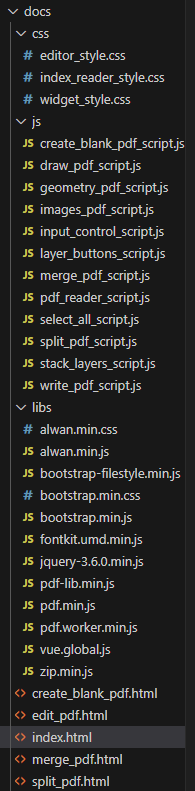
\includegraphics[width=0.3\textwidth]{"images/folders.png"}
	\caption{Ordnerstruktur der PDF Web App}
	\label{fig:folders}
\end{figure}

Im Ordner js sind meine selbst geschriebenen JavaScript-Dateien und im Ordner css meine eigenen CSS-Dateien abgelegt. Genauso wurden alle HTML-Dateien von mir erstellt. Der Ordner libs enthält alle JavaScript- und CSS-Dateien von externen Libraries. Die Datei pdf.worker.min.js ist eine dependency von pdf.js und fontkit.umd.min.js gehört zur Library PDF-LIB, um benutzerdefinierte Fonts einzubinden. Im Prinzip hat jedes Modul seine eigene JavaScript-Datei. Das Script input\_control\_script.js, welches alle Module implementiert, enthält Kontrollfunktionen für Benutzereingabefelder und die ZIP-Download-Funktionen. Der Editor enthält teilt sich die Dateien pdf\_reader\_script.js und index\_reader\_style.css mit dem Reader. Die CSS-Datei widget\_style.css deckt den Creator, Merger und Splitter ab. Der Editor besteht aus mehreren Scripten: write\_pdf\_script.js für Textelemente, draw\_pdf\_script.js für Zeichnungen, geometry\_pdf\_script.js für Shapeelemente, images\_pdf\_script.js für Bildelemente, layer\_buttons\_script.js für Ebenenmenübuttons, select\_all\_script.js für die Auswahlfilterbuttons Select All und Deselect All und stack\_layers\_script.js für Ebenenmanagementfunktionen. Der Reader, Splitter und Merger bestehen aus einer separaten HTML-Seite. Das Editormodul ist eine einzelne HTML-Seite, bei der je nach Funktion die entsprechenden Schaltflächen für die Elementoperationen mit display: flex eingeblendet und mit display: none ausgeblendet werden. 

\subsection{Layoutgestaltung}
Das Hauptmenü wollte ich sehr simpel und minimalistisch gestalten. Daher habe ich für die Startseite nur einen weißen Hintergrund mit einem oberen Balken in der Farbe \#333 als dunkles Grau, das die Hauptmenübuttons hervorhebt. Dieses dunkle Grau wird auch für die beiden oberen Reader-Leisten und den Reader Hintergrund verwendet. Die Buttons haben einen vordefinierten Style von der Library Bootstrap. In der Bootstrap Library kann man den Style durch bestimmte Klassen auswählen. Alle grünen Buttons in der PDF Web App und die Selection Menus im Creator und Splitter haben die Bootstrap-Klasse btn-success und der dunkle Button mit grüner Schrift und Umrandung des ausgewählten Hauptmenü-Buttons hat die Bootstrap Klasse btn-outline-success. Anfangs war es schwierig den default Style des input type="file" HTML-Elements zu überschreiben. Vor allem die Beschriftung des Buttons für Choose file war standardmäßig in Deutsch gehalten und lies sich nicht in englischer Sprache programmieren. Daher habe ich die Library Bootstrap Filestyle verwendet, um den Choose file Button in Englisch und mit einem Bootstrap-Style zu versehen. Um eine Designkonsistenz zu erzielen, habe ich die Bootstrap Buttons überall in der PDF Web App in verschiedenen Stylevarianten verwendet. Lediglich beim Tools Seitenmenü im Editor habe ich einen eigenen Style für die Buttons für Elementoperationen programmiert. Diese weißen Buttons haben eine schwarze Schrift mit einer Border Width von 2 Pixeln, Border Radius von 5 Pixeln und einer Border Color von \#333. Der inaktive weiße Modus-Button und die ausgeschalteten Selection Filter im Layers Menu hat den Bootstrap-Style btn-light und alle dunkelgrauen Buttons haben den Bootstrap-Style btn-dark. Alle rosa Flächen in der PDF Web App und ausgewählte Ebenen haben die Farbe \#dabdb6. Der hellgraue Operations Bar und das Namensfeld einer Ebene im Editor haben eine Farbe von \#8c8c8c. Tools und aktivierte Checkboxen haben eine türkise Hintergrundfarbe in \#5eb873. Der Hintergrund der Ebenen sowie die Seitengruppe für Layers einer Seite und das Tools Seitenmenüs hat einen Alphawert von 0.8. Abgewählte Ebenen, Selection Menus in Tools, der Hintergrund beim Output-Dateinamen und ausgewählte Dateinamen im Merger sind schwarz. Alle horizontalen Leisten mit Operationen haben eine Höhe von 58 Pixeln und dessen Buttons haben einen horizontalen Abstand von 5 Pixeln. Layers und Tools sind jeweils 190 Pixel breit. Hat man in Tools eine Font- oder Bilddatei ausgewählt, so wird nach 15 Zeichen im Dateinamen ein Zeilenumbruch eingefügt. Der Dateiname des Output-PDFs ist auf 50 Zeichen beschränkt. Im Reader befinden sich zwischen den gerenderten PDF-Seiten 20 Pixel Abstand. Alle input fields, Scrollbars und input type="checkbox" HTML-Elemente haben den default Style des Browsers. Die default Dateinamen für Reader und Editor sind wie folgt benannt: Source Dokument Dateiname, ein Unterstrich und edited. Der Creator besitzt den Dateinamen blank\_pdf und der Merger merged\_pdf. Im Splitter wird ebenfalls wie im Reader und Editor der Source Dateiname, ein Unterstrich und split verwendet. 

\subsection{Input Control}
Eine automatisierte Eingabekontrolle von Benutzereingabefeldern findet in allen Modulen, außer dem Merger, statt. Alle input fields sind input type="text" Elemente, anstatt type="number", selbst wenn nur Zahlen als Eingabewerte gültig sind. Das hat folgenden Hintergrund: Es gibt eine Funktion namens restrictInputValues, die automatisch Benutzereingaben korrigiert. Die Funktion wird ausgelöst, wenn das input field verändert wurde (change-Event). Im Prozess wird der event handler zunächst entfernt, bevor er aktiviert wird. Würde man den Event-Handler nicht zuallererst entfernen, so würde dieses Eingabefeld immer mehr Event-Handler akkumulieren. RestrictInputValues entfernt white space, wandelt die Benutzereingaben als String in Zahlen um und hält die eingegebenen Werte in einem gültigen Wertebereich. Außerdem gibt es eine Funktion convertInputToSuccess, die den Input-String in einen Zahlenwert parst und den geparsten Wert oder -1000 für eine ungültige Benutzereingabe zurückgibt. Die return value von convertInputToSuccess bestimmt maßgeblich, ob Operationen, z.B. die Schriftgröße im Texteditor ausgeführt werden sollen. Für die Eingabe von eine Liste an Seiten, gibt es eine gesonderte Funktion convertPagelistToSuccess. Hier wird im Falle von ungültigem Input die Benutzereingabe gelöscht. Eine genauere Beschreibung des Verhaltens der Input Control werde ich im Unterkapitel Testdurchführung, Abschnitt Testauswertung, weiter ausführen.

\subsection{Einlesen einer PDF-Datei}
Die Funktion für den Choose file Button ist im folgenden Codeabschnitt \ref{code:file} dargestellt:

\begin{lstlisting}[style=ES6, caption={Einlesen einer PDF-Datei}, label=code:file, breaklines=true]
	let inputFileButtons = document.getElementsByClassName('inputfile');
	for (let i = 0; i < inputFileButtons.length; i++) {
		inputFileButtons[i].addEventListener("change", function(e) {
			resetAllModes();
			// ...
			file = e.target.files[0];
			const fileReader = new FileReader(); 
			fileReader.onload = function() {
				const typedarray = new Uint8Array(this.result);
				const pdfBytes = typedarray;
				const loadingTask = pdfjsLib.getDocument(typedarray);
				loadingTask.promise.then(async (pdf) => {
					if (file.name.endsWith(".pdf")) {
						try {
							outputPDF = await PDFLib.PDFDocument.load(pdfBytes);
						} catch(encryptedErr) {
							encrypted = true;
						}
						if (!encrypted) {
							if (pdf._pdfInfo.numPages <= 5000) {
								pdfState.pdf = pdf;
								pdfState.originalPDFBytes = pdfBytes;
								pdfState.existingPDFBytes = pdfBytes;
								// ...
								pdfState.lastPage = pdf._pdfInfo.numPages;
								// ...
								adjustPDFToUserViewport();
								pdfState.renderedPage = 0;
								// ...
								let readerMode = true;
								let editorMode = false;
								const openPDFs = document.getElementsByClassName("open_pdf");
								for (let i = 0; i < openPDFs.length; i++) {
									if (openPDFs[i].classList.contains("btn-outline-success")) {
										readerMode = true;
										break;
									} else if (openPDFs[i].classList.contains("btn-success")) {
										readerMode = false;
									}
								}
								const editorBtns = document.getElementsByClassName("editor_btn");
								for (let i = 0; i < editorBtns.length; i++) {
									if (editorBtns[i].classList.contains("btn-outline-success")) {
										editorMode = true;
										break;
									} else if (editorBtns[i].classList.contains("btn-success")) {
										editorMode = false;
									}
								}
								if (!readerMode && editorMode) {
									onetimeSetup = true;
									// ...
									setTimeout(initEditor, 300);
								}
								startRender = performance.now();
								await renderPage(pageCounter, false);
							} else {
								pagesError = true;
								for (let i = 0; i < pagesErrorWidgets.length; i++) {
									pagesErrorWidgets[i].style.display = "flex";
								}
							}
						} else {
							encryptedError = true;
							for (let i = 0; i < encryptedErrorWidgets.length; i++) {
								encryptedErrorWidgets[i].style.display = "flex";
							}
						}
					}
				}).catch(unsupportedFileErr => {
					noPDFError = true;
					for (let i = 0; i < noPDFErrorWidgets.length; i++) {
						noPDFErrorWidgets[i].style.display = "flex";
					}
				});
			}
			if (file) {
				fileLoaded = true;
				fileReader.readAsArrayBuffer(file);
			}
		}, false);
	}
\end{lstlisting} 

Bei jedem Klick des Choose File Buttons werden alle Modi für aktive Operations-Buttons des Editors und andere Steuerungsmodi in der Funktion resetAllModes auf false gesetzt. Ich lese die Datei mit einem FileReader Objekt ein und führe beim load event eine Funktion aus, die am Ende das Rendern der Seiten anstößt. Die eingelesene PDF-Datei, bestehend aus einem Uint8Array, wird im Objektattribut originalPDFBytes und existingPDFBytes des globalen Objekts pdfState speichert. Die PDF-LIB-Funktionen für das Laden eines PDFs akzeptiert einen Parameter als Uint8Array und das Speichern gibt ein als Uint8Array serialisiertes PDF zurück. OriginalPDFBytes benötige ich für die Einbettung von Elementen im Editor. Im Editor wird bei jedem Downloadvorgang des modifizierten PDFs das originale PDF aus Grundlage zur Einbettung verwendet. 

Das Objekt pdfState, das den aktuellen Anzeige- und Datenstatus des eingelesenen PDFs repräsentiert, ist im Codeschnipsel \ref{code:pdfstate} dargestellt:

\begin{lstlisting}[style=ES6, caption={Objekt für den Status eines geöffnetes PDF-Dokuments}, label=code:pdfstate, breaklines=true]
	let pdfState = {
		pdf: null,
		currentPage: 1,
		lastPage: 1,
		renderedPage: 0,
		zoom: 1,
		originalPDFBytes: null,
		existingPDFBytes: null,
		originalWidths: [],
		originalHeights: []
	}
\end{lstlisting} 

Eine loadingTask wird durch die pdf.js Funktion getDocument erzeugt, die ein libraryinternes pdf Objekt zurückliefert. Dieser Return Wert wird in pdfState.pdf abgelegt und in pdfState.lastPage wird die Seitenzahl der letzten Seite gespeichert. Das pdf.js pdf-Objekt wird für das Rendern der PDF-Seiten im Reader benötigt. Weiter im Code wird das PDF dem Viewport des Browsers angepasst. Eine Anpassung erfolgt nur, wenn die Breite der ersten Seite des geöffneten Dokuments größer als der Viewport des Browsers ist. Dann wird der Zoomfaktor entsprechend angepasst, sodass die Seite mit einem Rand von 100 Pixeln formatfüllend in den Viewport passt. Anschließend wird pdfState.renderedPage initialisiert. Dieses property enthält die aktuell gerenderte Seite, die am Ende des Rendervorgangs der letzten Seite des PDFs entspricht. Ob es sich um den Reader oder Editor handelt, wird überprüft, indem ich die Bootstrap-Klassen der zugehörigen Hauptmenü-Buttons ermittle. Falls der Editor geöffnet wurde, wird er mit einer Zeitverzögerung von 300 ms aufgebaut. Hintergrund dessen ist, dass die vorherige \gls{dom}-Version erst gerendert werden muss, sonst erhält man bei Zugriff auf HTML-Collections – ein arrayähnliches Objekt – eine Länge von Null. Am Ende wird der Rendervorgang durch die rekursive, asynchrone Funktion renderPage in Gang gesetzt. Das \gls{dom} ist eine Web \gls{api} für Webdokumente wie HTML-Dokumente. Es repräsentiert die Webseite als nodes und Objekte, sodass Programmiersprachen die Dokumentenstruktur, -style und -inhalt modulieren können. Strukturell besteht das \gls{dom} aus dem \gls{dom} tree, dessen nodes den HTML-Inhalt repräsentieren. Im \gls{dom} sind alle properties, Methoden und events für die Manipulation und Erzeugung von Webseiten als Objekte organisiert \cite{mozilla-dom}. 

\subsection{Renderfunktion}
Die Funktion renderPage ist im Codeauszug \ref{code:render} abgebildet.

\begin{lstlisting}[style=ES6, caption={Renderfunktion}, label=code:render, breaklines=true]
	async function renderPage(num, renderSingle) {
		pdfState.pdf.getPage(num).then(function(page) {
			let viewport = page.getViewport({
				scale: pdfState.zoom
			});
			let viewportOriginal = page.getViewport({
				scale: 1
			});
			let canvas;
			let div;
			const pdfViewers = document.getElementsByClassName("pdf_viewer");
			for (let i = 0; i < pdfViewers.length; i++) {
				const pdfViewer = pdfViewers[i];
				// ...
				if (writeLayerStack.length < pdfState.pdf._pdfInfo.numPages) {
					div = document.createElement("div");
					div.style.display = "flex";
					div.width = viewport.width;
					div.height = viewport.height;
					div.style.width = viewport.width + "px";
					div.style.height = viewport.height + "px";
					div.style.marginBottom = "20px";
					pdfState.originalWidths.push(viewportOriginal.width);
					pdfState.originalHeights.push(viewportOriginal.height);
					div.setAttribute('data-write', pageCounter);
					div.classList.add("write_layer");
					canvas = document.createElement("canvas");
					canvas.style.display = "flex";
					canvas.width = viewport.width;
					canvas.height = viewport.height;
					canvas.style.width = viewport.width + "px";
					canvas.style.height = viewport.height + "px";
					canvas.setAttribute('data-page', pageCounter);
					canvas.classList.add("render_context");
					div.appendChild(canvas);
					pdfViewer.appendChild(div);
					writeLayerStack.push(div);
				} else if (writeLayerStack.length === pdfState.pdf._pdfInfo.numPages) {
					if (!renderSingle) {
						div = writeLayerStack[pageCounter-1];
						canvas = writeLayerStack[pageCounter-1].childNodes[0];
					} else {
						div = writeLayerStack[num-1];
						canvas = writeLayerStack[num-1].childNodes[0];
					}
					div.width = viewport.width;
					div.height = viewport.height;
					div.style.width = viewport.width + "px";
					div.style.height = viewport.height + "px";
					canvas.width = viewport.width;
					canvas.height = viewport.height;
					canvas.style.width = viewport.width + "px";
					canvas.style.height = viewport.height + "px";
				}
			}
			const context = canvas.getContext('2d');
			let renderTask = page.render({
				canvasContext: context,
				viewport: viewport
			});
			if (!renderSingle) {
				renderTask.promise.then(function() {
					pdfState.renderedPage = pageCounter;
					// ...
					pageCounter++;
					// ...
					if (pdfState.pdf != null && pageCounter <= pdfState.pdf._pdfInfo.numPages) {
						renderPage(pageCounter, false);
					}
				});
			}
		});
	}
\end{lstlisting} 

Die Funktion ruft sich rekursiv auf, falls noch nicht alle Seiten gerendert wurden. Sie kann für das Rendern auf ein oder mehreren Seiten operieren. Pro Funktionsaufruf wird der globale pageCounter hochgezählt. Mittels des pdfState.pdf-Objekts wird die aktuelle Seite geholt und ein Seitenobjekt von pdf.js entgegengenommen. Vom Seitenobjekt wird der Viewport der Seite geholt und eine Skalierung festgelegt. Das pdfState property zoom, was die aktuelle Skalierung des gesamten PDF-Dokuments speichert wird der Viewport-Skalierung zugewiesen. Viewport besitzt width und height properties. Zusätzlich wird der Viewport mit einer Skalierung von 1 geholt, damit im weiteren Verlauf von renderPage die Arrays pdfState.originalWidths und pdfState.originalHeights die Originalgröße der PDF-Seite aufnehmen können. Der Container des gerenderten PDFs besteht aus mehreren verschachtelten DIV-HTML-Elementen, wobei das innere Element die Klasse pdf\_viewer besitzt. Dem inneren PDF-Viewer-Container werden pro Ausführung von renderPage ein DIV mit der Klasse write\_layer und einem data-Attribut data-write, was die aktuelle Seitenzahl speichert, hinzugefügt. Die Write Layer symbolisiert einen Seitencontainer, der die gerenderte PDF-Seite und beigefügten Elemente des Editors enthält. Die gerenderte PDF-Seite wird in einem Canvas-Element als erstes Child der Write Layer hinzugefügt. Diese Canvas hat die Klasse render\_context und ein data-Attribut data-page für die aktuelle Seitenzahl. Sowohl die Write Layer als auch der Render Context werden in der Größe des aktuell skalierten Viewports angelegt. Die Write Layer wird zusätzlich in einem Array writeLayerStack abgelegt. WriteLayerStack hält die Write Layers in der Reihenfolge der PDF-Seiten im Dokument. Während eines erneuten Rendervorgangs wird aus diesem Array der Render Context herausgeholt und wiederverwendet. Dann wird mittels der pdf.js-Library die Seite gerendert und nach der renderTask wird eine anonyme Funktion ausgeführt. Nachdem die Seite in den Render Context geschrieben wurde, wird pdfState.renderedPage die pageCounter Variable zugewiesen. Dieses property wird dann als Maximalwert für die Input Control bei der Navigation zu einer bestimmten Seite verwendet. Folglich kann der User nur zu einer Seite springen, die ihm bereits angezeigt wird. 

\subsection{Implementierung der Vue JS 3-Module}
Die Module Creator, Splitter und Merger verwenden das Framework Vue JS 3, zwar nicht in nativer Form als \gls{spa}, jedoch wird Vue JS 3 als stand-alone widgets in diese Module integriert. Beim Creator wird annähernd die eingestellte PDF-Seitengröße als Breite und Höhe der MediaBox durch die Berechnung in den Codezeilen \ref{code:mediabox}, die ich durch Ausprobieren herausgefunden habe, gesetzt.

\begin{lstlisting}[style=ES6, caption={Berechnung der PDF-Seitengröße}, label=code:mediabox, breaklines=true]
const pageWFactor = (blankPageWidth * 1000) / 352.8;
const pageHFactor = (blankPageHeight * 1000) / 352.8;
for (let i = 0; i < blankNumOfPagesCount; i++) {
	page = pdfDoc.addPage();
	page.setMediaBox(0, 0, pageWFactor, pageHFactor);
}
\end{lstlisting} 

Beim Anklicken der Portrait-Orientierung wird in den Width and Height input fields der kleinere Wert der Seitendimensionen für die Width gesetzt und der größere Wert für die Height. Im Falle von Landscape werden Width und Height vertauscht und Quadratic orientiert sich an der Width.
\par
Wenn man den Splitter öffnet findet man zunächst einen gesperrten Save-Button vor. Der Save-Button wird erst benutzbar, wenn man eine PDF-Datei und Split-Methode im selection menu ausgewählt hat. Der Dateiname, begrenzt auf 50 Zeichen, wird unter dem Choose file-Button abgebildet. Die Methode list of pages kann man auch zum Splitten nach einer bestimmten Seite verwenden. Erst wenn man diesen Menüpunkt ausgewählt hat, wird das input field für die Seitenliste aktiviert. Die Split-Funktion fürs Splitten nach geraden und ungeraden Seiten heißt SplitAfter. Basierend auf den Rest Modulo 2 wird die Funktion nur ausgeführt, wenn bei der even pages-Split-Methode mehr als 3 Seiten im Input-PDF vorliegen bzw. bei der odd pages-Split-Methode mehr als 2 Seiten vorhanden sind. Andernfalls wird der Save-Button ebenfalls deaktiviert. Die Input-PDF Bestandteile als Dokumentobjekte von PDF-LIB, die nach jedem Split-Vorgang bei der PDF-LIB-Funktion PDFDocument.create entstehen, werden in einem globalen Array splittedPDFs gesichert. Die Arraybestandteile werden durch Klick auf Save einzeln zu einem Uint8Array serialisiert und in einem globalen Array pdfBytesList gespeichert. PdfBytesList wird dann der compressMultipleToZip funktion übergeben. Jedes gesplittete PDF enthält den Ursprungsdateinamen, einen Unterstrich und einen Index beginnend mit 0, der das Teil-PDF in der Split-Reihenfolge aufsteigend nummeriert. Alle Source-PDF-Bestandteile werden in einen ZIP-Ordner verpackt. Am Ende des Downloads werden splittedPDFs und pdfBytesList wieder als leeres Array gesetzt.
\par
Im Merger wird eine geöffnete Datei als Uint8Array einem globalen Array selectedPDFBytes hinzugefügt. Zusätzlich wird einem UL-HTML-Element, dem Dateilistencontainer, pro Datei ein LI-HTML-Element mit der Klasse file\_unselected, sowie dem Dateinamen gekürzt auf 50 Characters und einem click Event Handler für die Dateimarkierung, hinzugefügt. Erst wenn man mehr als 1 Datei oder maximal 100 ausgewählt hat werden der Save- und Remove-Button funktionstüchtig gemacht. Außerdem wird dem LI eine Reihe an drag-Events hinzugefügt: dragstart, dragover und drop. Funktion der drag-Events ist, dass der Benutzer die Listeneinträge in ihrer Reihenfolge verschieben kann. Dabei spiegelt selectedPDFBytes die Reihenfolge der Listeneinträge wieder. Für das dragging muss der Listeneintrag nicht markiert sein, jedoch beim Entfernen von einzelnen Listeneinträgen schon. Ist ein Listeneintrag schwarz markiert, so wird die Klasse file\_unselected vom entsprechenden LI entfernt und stattdessen die Klasse file\_selected hinzugefügt. Hat man so viele Listeneinträge entfernt, dass nur noch 1 oder keine Datei übrig bleibt, so wird Save abermals gesperrt. Ebenso wird Remove bei keinen Elementen deaktiviert.

\subsection{Struktur der Editorelemente}
Die 4 Editorelemente Text, Drawing, Shape und Image werden bei Erzeugung auf der Seite in 4 zugehörigen globalen Arrays in der Erstellungsreihenfolge abgelegt: userTextList für Text, drawLayerStack für Drawings, geometryPointsList für Shapes und userImageList für Images. Für die Erstellung der Editorelemente verwende ich zum einen Objekt, die die Node-Struktur der Elemente in der Webseite abbilden und zum anderen Objekte, die die elementspezifischen Eigenschaft repräsentieren. Diese Objekte werden nicht direkt verwendet, sondern sie werden als Prototypen nach dem Konzept der prototypischen Objektorientierung für die Erstellung konkreterer Objekte verwendet, die vom Prototyp erben. Im Codeabschnitt \ref{code:control-point} ist das strukturelle Prototyp-Objekt für Text, Drawing und Image abgebildet. Der darauffolgende Codeabschnitt \ref{code:shape-controller-point} zeigt das strukturelle Prototyp-Objekt für Shape.

\begin{lstlisting}[style=ES6, caption={Prototyp-Objekt für die Node-Struktur von Text, Drawing und Image}, label=code:control-point, breaklines=true]
	let controlPoint = {
		controlBox: null,
		editImg: null,
		elementToControl: null,
		type: '',
		layer: null,
		page: 1,
		x: 0,
		y: 0,
		index: 0,
		setControlPoint() {
			let div = document.createElement("div");
			div.style.position = "absolute";
			div.style.left = this.x + "px";
			div.style.top = this.y + "px";
			div.setAttribute('data-page', this.layer.getAttribute("data-write"));
			div.setAttribute('data-index', this.index);
			div.classList.add(this.type);
			div.classList.add("box");
			this.controlBox = div;
		}
	}
\end{lstlisting}

\begin{lstlisting}[style=ES6, caption={Prototyp-Objekt für die Node-Struktur von Shape}, label=code:shape-controller-point, breaklines=true]
	let shapeControllerPoint = {
		controlBox: null,
		editImg: null,
		elementToControl: null,
		layer: null,
		page: 1, 
		x: 0,
		y: 0,
		index: 0, 
		rotation: 0,
		originX: 0,
		originY: 0,
		setControlPoint() {
			let div = document.createElement("div");
			div.style.position = "absolute";
			div.style.left = this.x + "px";
			div.style.top = this.y + "px";
			div.setAttribute('data-page', this.layer.getAttribute("data-write"));
			div.setAttribute('data-index', this.index);
			div.classList.add("shape");
			div.classList.add("box");
			this.controlBox = div;
		},
		rotateControlPoint() {
			this.controlBox.style.marginLeft = this.originX + "px";
			this.controlBox.style.marginTop = this.originY + "px";
			this.controlBox.style.transform = "rotate(" + this.rotation + "deg)";
		}
	}
\end{lstlisting}  

Vom controlPoint-Prototyp leitet das Objekt controlP ab und von shapeControllerPoint leitet shapeControllerP ab. ShapeControllerPoint stellt einen spezialisierten controlPoint dar, der mit Rotationseigenschaften erweitert wurde. ControlP und shapeControllerP-Objekte werden direkt in userTextList, drawLayerStack, userImageList und geometryPointsList gespeichert.
Die Prototypen besitzen ein Attribut elementToControl, um die Objekte mit elementspezifischen Eigenschaften zu speichern. Dessen Prototypen heißen userText für Text, drawLayer für Drawings, shape für Shapes und userImage für Images. Sie sind in den Codesegmenten aufgeführt.

\begin{lstlisting}[style=ES6, caption={Prototyp-Objekt für die textspezifischen Eigenschaften}, label=code:user-text, breaklines=true]
	let userText = {
		pdfDoc: null,
		pdfBytes: null,
		text: '',
		x: 1,
		y: 1,
		size: 1,
		fontKey: null,
		font: null,
		lineHeight: 34,
		color: rgb(0, 0, 0),
		page: 1,
		opacity: 1.0,
		rotation: degrees(0),
		setTextElem() {
			this.pdfDoc.getPages()[0].drawText(this.text, {
				x: this.x,
				y: this.y,
				size: this.size,
				font: this.font,
				color: this.color,
				lineHeight: this.lineHeight,
				rotate: this.rotation
			});
		}
	}
\end{lstlisting}

\begin{lstlisting}[style=ES6, caption={Prototyp-Objekt für die drawingspezifischen Eigenschaften}, label=code:draw-layer, breaklines=true]
	let drawLayer = {
		paths: [],
		currentPathIndex: 0, 
		rotation: 0,
		wasRotated: false
	}
\end{lstlisting}

\begin{lstlisting}[style=ES6, caption={Prototyp-Objekt für die shapespezifischen Eigenschaften}, label=code:shape, breaklines=true]
	let shape = {
		context: null,
		type: "",
		x: 0,
		y: 0,
		xp2: 50,
		yp2: 50,
		width: 100,
		height: 100,
		stroke: 'rgba(0,0,0,1.0)',
		strokeWidth: 3,
		fill: '',
		useFill: false,
		useStroke: false,
		rotation: 0,
		page: 1,
		drawShape() {
			if(this.type === "rectangle") {
				let rectCenterX = this.x + this.width / 2;
				let rectCenterY = this.y + this.height / 2;
				this.context.save();
				this.context.beginPath();
				this.context.translate(rectCenterX, rectCenterY);
				this.context.rotate(this.rotation * Math.PI / 180);
				this.context.translate(-rectCenterX, -rectCenterY);
				if (this.useFill) 
				this.context.fillStyle = this.fill;
				if (this.useStroke) {
					this.context.strokeStyle = this.stroke;
					this.context.lineWidth   = this.strokeWidth;
				}
				if (this.useFill) {
					this.context.fillRect(this.x, this.y, this.width, this.height);
				}
				if (this.useStroke) {
					this.context.strokeRect(this.x, this.y, this.width, this.height);
				}
				this.context.restore();
			} else if (this.type === "triangle") {
				let triCenterX = this.x + this.width / 2;
				let triCenterY = this.y + this.height / 2;
				this.context.save();
				this.context.beginPath();
				this.context.translate(triCenterX, triCenterY);
				this.context.rotate(this.rotation * Math.PI / 180);
				this.context.translate(-triCenterX, -triCenterY);
				this.context.moveTo(this.x, this.y);
				this.context.lineTo(this.x, this.y + this.height);
				this.context.lineTo(this.x + this.xp2 + this.width, this.y + this.yp2);
				this.context.closePath();
				
				if (this.useFill) 
				this.context.fillStyle = this.fill;
				
				if (this.useStroke) {
					this.context.strokeStyle = this.stroke;
					this.context.lineWidth   = this.strokeWidth;
				}
				
				if (this.useFill) 
				this.context.fill();
				
				if (this.useStroke)    
				this.context.stroke();
				
				this.context.restore();
			} else if (this.type === "circle") {
				this.context.beginPath();
				this.context.ellipse(this.x, this.y, this.width / 2, this.height / 2, this.rotation * Math.PI / 180, 0, 2 * Math.PI);
				
				if (this.useFill) {
					this.context.fillStyle = this.fill;
				}
				if (this.useStroke) {
					this.context.strokeStyle = this.stroke;
					this.context.lineWidth   = this.strokeWidth;
				}   
				this.context.closePath();
				if (this.useFill) {
					this.context.fill();
				}
				if (this.useStroke)    
				this.context.stroke();
			}
		}
	}
\end{lstlisting}

\begin{lstlisting}[style=ES6, caption={Prototyp-Objekt für die imagespezifischen Eigenschaften}, label=code:user-image, breaklines=true]
	let userImage = {
		pdfDoc: null,
		pdfBytes: null,
		image: null,
		base64String: "",
		type: "",
		x: 1,
		y: 1,
		width: 1,
		height: 1,
		page: 1,
		opacity: 1.0,
		rotation: degrees(0),
		setImageElem() {
			this.pdfDoc.getPages()[0].drawImage(this.image, {
				x: this.x,
				y: this.y,
				width: this.width,
				height: this.height,
				rotate: this.rotation,
			});
		}
	}
\end{lstlisting}

Die spezifischen Objekte zu ihren Prototypen heißen currentUserText für userText, drawingLayer für drawLayer, currentShape für shape und currentUserImage für userImage. Sowohl die Nodestrukturobjekte, als auch die Eigenschaftsobjekte werden beim Hinzufügen von Elementen erstellt und mit Standardwerten initialisiert. 

\subsection{Aufbau eines PDF-Seitencontainers}
Die Wurzel eines PDF-Seitencontainer bildet ein DIV mit der Klasse write\_layer. Die write\_layer hat mindestens ein child, eine Canvas mit der Klasse render\_context. Dieser Fall liegt vor, wenn man noch keine Elemente zum PDF hinzugefügt hat. Man kann sich den Render Context als Zeichenfläche vorstellen, die durch die Dimensionen der PDF-Seite begrenzt ist, mit dem gerenderten Seiteninhalt als Hintergrund. Sobald der Benutzer Elemente der Seite hinzufügt, werden weitere Schichten auf den Render Context gelegt, wobei ein Element aus einer Canvas, die ich editimg genannt habe, für die Darstellung und einem 40 x 40 Pixel-großen DIV namens controlBox für den Kontrollpunkt des Elements besteht. Die Canvas besitzt 3 Klassen: Editimg, visible und eine Elementtyp-Klasse. Die Klasse editimg bezeichnet die Canvas, die das gerenderte, einzelne Element enthält. Visible definiert den Sichtbarkeitsstatus für das Ein- und Ausblenden von Elementen über die Ebenensteuerung. Die Typklasse kann entweder text, drawing, shape oder image sein. Jedes editimg enthält außerdem ein data-page für die Seitenzahl und data-index für die Position in der Elementliste Attribut. Die Größe des editimgs entspricht immer der Größe des zugehörigen render\_contextes. Auf der controlBox habe ich eine Reihe von Event-Handler definiert, die die Operationen im Operations Bar und Tools ausführen. Sie besitzt eine Typklasse und die Klasse box, um alle controlBoxes im Dokument ansprechen zu können. Die controlBox besitzt ebenfalls die gleichen data-Attribute wie das zugehörige editimg. Die editimgs werden bei Erzeugung aufeinander gestapelt mit dem zuletzt erstellten editimg zuoberst. Alle editimgs werden in einem Gruppierungs-DIV mit der Klasse editimg\_group akkumuliert. Ebenfalls werden alle controlBoxes in einem gruppierenden DIV mit der Klasse control\_group vereint. Die editimg\_group liegt über dem render\_context. Ganz oben befindet sich die control\_group, damit Kontrollpunkte nicht von gerenderten Elementen verdeckt werden. Die control\_group und editimg\_group werden beim Hinzufügen des ersten Elementes auf der Seite erstellt. Jede write\_layer hat jeweils eine editimg\_group und control\_group. Das Node-Tree Segment für den Aufbau einer write\_layer ist in Screenshot \ref{fig:write-layer} veranschaulicht. 

\begin{figure}[!htbp]
	\centering
	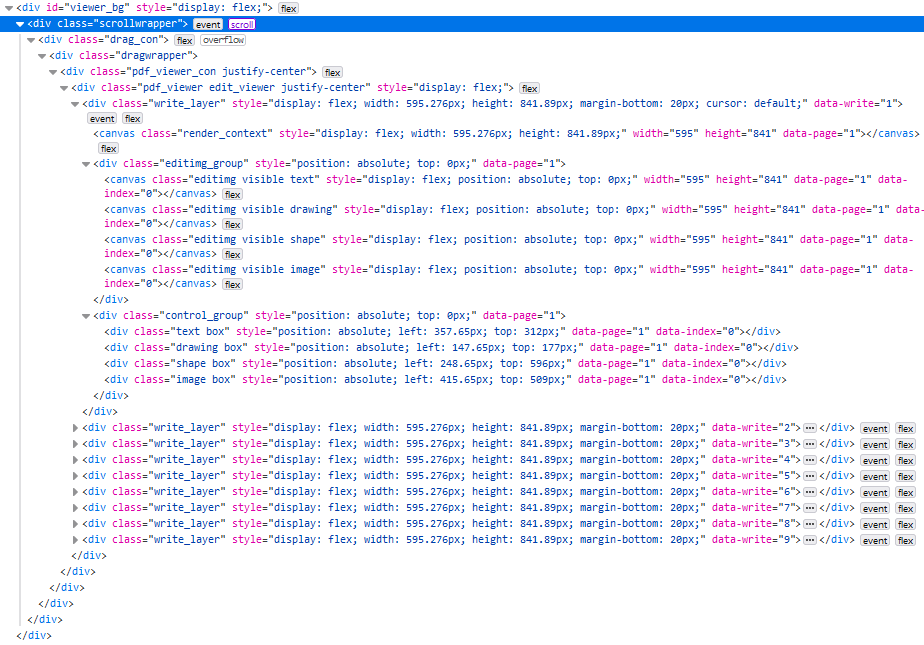
\includegraphics[width=1\textwidth]{"images/write-layer.png"}
	\caption{Node-Tree Segment für den Aufbau einer write\_layer mit 4 Elementen jedes Typs}
	\label{fig:write-layer}
\end{figure}

Für editimg und controlBox gibt es properties in den Nodestrukturobjekten. Dort wird die Canvas und das DIV abgespeichert. Außerdem gibt es ein layer property, in dem die zugehörige write\_layer gesichert wird. In den properties type wird der Elementtyp als String hinterlegt, page beschreibt die Seitenzahl, x und y sind die Koordinaten auf der Seite und index ist die Position des Elements in der zugehörigen Liste. Die Reihenfolge der Elemente in userTextList, drawLayerStack, geometryPointsList und userImageList ändert sich nie, es sei denn ein Element wird vom Benutzer gelöscht. Der index in den Nodestrukturobjekten muss immer mit data-index von editimg und controlBox übereinstimmen. Über diesen maßgeblichen index kann auf das Element in der jeweiligen Liste zugegriffen werden.

\subsection{Hinzufügen von Elementen}
Jedes Element hat seine separate Funktion, um es der Seite hinzuzufügen. Jede Funktion enthält die Funktion createStackLayer, um eine Layer für das Element zu erstellen. Am Ende jeder Funktion zum Hinzufügen wird das Nodestrukturobjekt der zugehörigen Liste hinzugefügt. Wenn Text hinzugefügt werden soll, wird der Text in Form des Eigenschaftsobjekt erstellt. Aus Sicht der Implementierung wird ein PDF-Dokument mit einer Seite mit PDF-LIB erstellt, worauf der Text an der Stelle, wo der Benutzer mit der Maus auf die Seite geklickt hat, platziert wird. Die einzelne PDF-Seite hat die Größe des render\_contextes bzw. der write\_layer, da der render\_context und die write\_layer die gleiche width und height haben. Dann wird diese Seite mit einem transparenten Hintergrund mit pdf.js in das editimg gerendert. Das Klick-Event ist mit der write\_layer verknüpft. Alle Funktionen zum Hinzufügen von Elementen sind an das Klick-Event auf der write\_layer gebunden. In die PDF-Seite wird der Standard-Font TimesRoman eingebettet. Im Eigenschaftsstrukturobjekt befindet sich die PDF-LIB-Funktion drawText und sie wird in addText mit Standardwerten gefüttert. Zu beachten ist, dass currentUserText.opacity nicht an drawText übergeben wird, da die opacity-Implementierung der PDF-LIB in der Library defekt zu sein scheint. Außerdem wird das Dokument-Objekt von PDF-LIB in currentUserText.pdfDoc abgelegt und die Uint8Array-Repräsentation des Dokuments ebenfalls. Die Seitenzahl wird in currentUserText.page abgelegt und die currentUserText.rotation mit 0 initialisiert. Alle Editor-Elemente werde bei der Erzeugung mit einer Rotation von 0 erstellt und alle Eigenschaftsobjekte haben ein page property. Des Weiteren wird der Textinhalt als String in currentUserText.text festgehalten, das Font-Objekt, das beim Einbetten des Fonts entsteht, in currentUserText.font, sowie die ArrayBuffer-Variante des, mit dem Dateibrowser geöffneten Fonts, in currentUserText.fontKey gespeichert. Text-Eigenschaftsobjekte sind die einzigen Eigenschaftsobjekte mit einem size Attribut.
\par
Die Funktion addImage funktioniert ähnlich wie addText. Das Image wird ebenfalls auf eine PDF-Seite platziert und mit transparentem Hintergrund in editimg gerendert. Im Vorgang wird das eingelesene Image, was in der Bilddateiliste in Tools ausgewählt wurde, in Form von Base64 in das einseitige PDF eingebettet. Zurückgegeben wird ein Bildobjekt von PDF-LIB, was in currentUserImage.image abgelegt wird. Das erzeugte PDF-Objekt wird in currentUserImage.pdfDoc und das Base64-Image in currentUserImage.base64String gespeichert. Shape- und Image-Eigenschaftsobjekte haben width und height Attribute. In currentUserImage befindet sich die setImageElem-Methode mit der drawImage-PDF-LIB-Funktion.
\par
Shapes und Drawings benötigen keine PDF-Dokumentseite bei ihrer Entstehung. Der shapeControllerP besitzt noch properties rotation, originX, originY und eine Funktion rotateControlPoint, um die controlBox mit dem Shape gemeinsam im gleichen Winkel zu drehen. In der Funktion addShape wird der Shape direkt auf das editimg mit Canvas-Funktionen für Rechtecke und Ellipsen gezeichnet. Dreiecke müssen durch einzelne Linien gezeichnet werden. In currentShape.context wird der Canvas 2D-Rendering-Context gespeichert. Er wird für die Zeichenoperationen verwendet. CurrentShape.type speichert den Shape-Typ als String. Die Typen heißen rectangle, triangle und circle. Die properties xp2 und yp2 stehen für den dritten Punkt des Dreiecks (Triangle's 3rd Point). Sie werden nur bei Erstellung von Triangles initialisiert und bei der Triangle's 3rd Point Operation verwendet. CurrentShape besitzt stroke, strokeWidth, fill, useFill und useStroke Attribute. UseFill und useStroke werden für die Steuerung der Checkboxen in der GUI bei Stroke Color und Fill Color in Tools verwendet. Man kann entweder nur eine Stroke Color oder nur eine Fill Color anwenden oder beide gleichzeitig. 
\par 
Die Funktion zum Hinzufügen von Drawings heißt draw und ist mit dem Klick-Event auf die write\_layers verbunden. Im drawLayer.paths-Array werden die Pfadpunkte des Zeichenvorgangs angehängt. Zuerst wird geprüft, ob sich auf der Seite schon ein Drawing befindet, falls nicht wird ein controlP und eine drawingLayer erstellt. Sie wird ebenfalls erstellt, wenn der Benutzer New Layer gedrückt hat. Gezeichnet wird auf der selektierten Layer. Wenn keine DrawingLayer selektiert ist wird standardmäßig auf der zuletzt gezeichneten Layer der Seite gemalt. Bei der Erstellung der Pfadsegmente wird, wie bei Shape, direkt auf dem context des editimgs gezeichnet und in drawingLayer.paths wird ein Objekt mit den x, y, line, color und compositeOp properties hinzugefügt. DrawingLayer.currentPathIndex dient der Traversierung von paths. Gezeichnet wird mit einem context.lineCap "round" und context.lineJoin "round" Linienaussehen, d.h. die Linie ist abgerundet an ihren Enden. Die context.globalCompositeOperation ist "source-over". Beim Radieren wäre sie "destination-out". Diese globalCompositeOperation wird in compositeOp in paths vermerkt. Die erase-Funktion funktioniert ähnlich wie draw, nur dass keine Layers, controlPs und DrawingLayers erstellt werden. Diese Objekte werden nur in draw erstellt.


\subsection{Erzeugung von Layers}
Die Layer zum zugehörigen Element wird in dessen Erstellungsmethode addText, addShape, addImage oder draw erzeugt. Die Funktion heißt createStackLayer. Anfangs ist die Layer nicht ausgewählt und nicht gesperrt. Dies wird durch die Klassen layer\_unselected und unlocked angezeigt. Die Klassen werden einem DIV mit der Klasse layercontainer hinzugefügt. Layercontainer hat außerdem ein data-page, data-index und data-type Attribut. Page entspricht der zugehörigen Seitenzahl, index dem Editorelementindex in der Liste und type kann entweder text, drawing, shape oder image sein. Alle weiteren HTML-Elemente im layercontainer sind mit den gleichen data-Attributen versehen. In createStackLayer werden Event-Listener an HTML-Elemente von layercontainer gebunden. Die checkbox ist mit einer Funktion hideLayer und einem input-Event verknüpft und das input-HTML-Element mit der Klasse layername für den editierbaren Layernamen hört auf die Funktion markLayer mit einem Klick-Event. Das DIV mit der Id layer\_stack\_con wird mit einer Funktion moveLayer verknüpft, die dragstart-, dragover- und drop-Events enthält, damit man die Layers in ihrer Reihenfolge verschieben kann, was bewirkt dass die Editorelemente Richtung Vordergrund oder Hintergrund verschoben werden in ihrer z-Achsenreihenfolge. Außerdem wird die neu erzeugte Layer mit dem aktuellen Element automatisch in Rosa markiert. Abbildung \ref{fig:layer:stack} zeigt den Aufbau der HTML-Elemente des layer\_stacks.

\begin{figure}[!htbp]
	\centering
	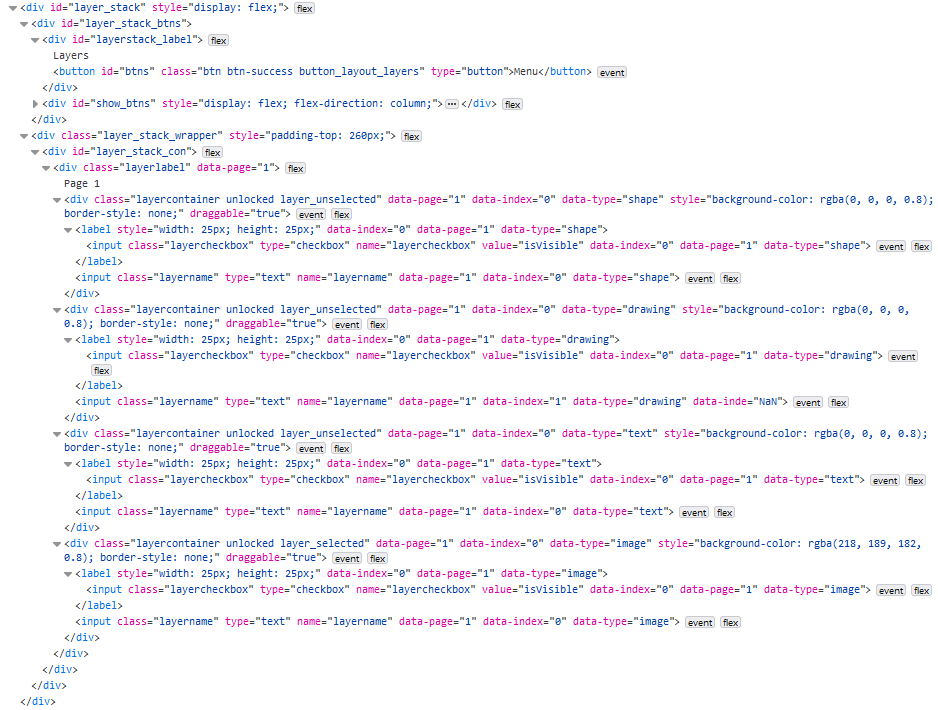
\includegraphics[width=1\textwidth]{"images/layer-stack.png"}
	\caption{Node-Tree Segment für den Aufbau der Layers}
	\label{fig:layer-stack}
\end{figure}

Beim Kopieren von Layers, was die Funktion dublicateLayerByElement hervorruft, wird zunächst die Layer per cloneNode(true) dubliziert und erhält einen inkrementierten Index in seinen data-index Attributen, d.h. wenn es bereits 3 Textelemente gibt und eins davon dubliziert wird, erhält das dublizierte Element und die Layer den Index von 3 (Index startet bei 0). Die dublizierte Layer wird hinter der source Layer eingefügt im layer\_stack. Folglich liegt das kopierte Element über dem source Element in der z-Achsenreihenfolge. Außerdem wird der kopierten Layer ein input-Event mit der hideLayer-Funktion und ein Klick-Event mit der markLayer-Funktion angeheftet. Zusätzlich wird erneut moveLayer auf dem layer\_stack\_con ausgeführt, damit die drag-Events auf der neuen Layer ausführbar sind. Die Funktion dublicateElement kopiert das Element der dublizierten Ebene. Dabei wird das Nodestrukturobjekt aus seiner Liste geholt und anhand dessen ein neues Nodestrukturobjekt samt Eigenschaftsobjekt erzeugt und dessen properties werden mit den Werten der source-Objekte initialisiert. Bei kopierten drawingLayer-Objekten ist zu beachten, dass das Objekt mit der deepCopy-Funktion nicht nur die Referenzen kopiert, sondern tatsächlich das Objekt und alle Unterobjekte in paths. Das kopierte Objekt wird seiner Liste hinzugefügt und die source Layer bleibt ausgewählt, während die kopierte Layer nicht ausgewählt ist. Gesperrte kopierte Objekte bleiben gesperrt.

\subsection{Box Mode Modi}
Bei jeder Operation auf einem Element im Operations Bar und Tools, außer bei den Operationen zum Hinzufügen von Elementen wird zunächst geprüft, ob der User sich im Box Mode oder layer Mode befindet und, ob die Layer locked ist. Alle Operationen im Box Mode besitzen einen Modus. Jeder Modus wird mit seinem Boolean-Wert in einem Modi-Array festgehalten. Die Modusliste für Operationen auf Text heißt userModes, für Drawings userModesDrawer, für Shapes userModesGeometry und für Images userModesImages. Bei den meisten Buttons im Reader und Editor wird eine Funktion resetAllModes ausgeführt. Sie setzt alle Modilistenbestandteile auf false. Dadurch kann der Benutzer einen Operationsmodus verlassen, wenn er eine andere Operation ausführt und in ihren Modus gelangen. Somit kann der Benutzer beispielsweise mehrere Textelemente mit einem Click auf Font Color in Rot färben, ohne erneut auf Font Color klicken zu müssen. Der zugehörige Modus der Operation wird im Event-Handler auf true gesetzt, falls der Benutzer sich im Box Mode befindet.

\subsection{Zoomfunktionalität}
Bei den Zoom Operationen ist eine Verzögerung von 300 ms eingebaut. Das liegt daran, dass man nicht zu schnell hintereinander Zoomen sollte, da sonst ein Fehler geworfen wird, dass man nicht gleichzeitige Renderoperationen auf dem gleichen Canvas-HTML-Element ausführen kann. Bei den Funktionen zoomIn, zoomOut und enterZoomFactor wird erst eine Funktion namens placeEditorElements ausgeführt, die die controlBoxes und Editorelemente passend zum Zoomfaktor auf der Seite platziert. Alle Editorelemente werden neu und verkleinert bzw. vergrößert gezeichnet. ControlBoxes behalten beim Zoomen ihre Größe bei. Danach werden alle Seiten mit dem neuen Zoomfaktor gerendert.

\subsection{Downloadfunktion}
Die Downloadfunktion für Editorelemente wird in einer promise-Chain ausgeführt. Zunächst wird der aktuelle Zoomfaktor gespeichert und das PDF-Dokument wird auf 500 \% Prozent vergrößert. Das hat den Hintergrund, dass alle Editorelemente anschließend als DataURL in Form eines PNG-Bildes in das PDF mit originalPDFBytes eingebettet werden. Genauer gesagt werden alle Canvas-HTML-Elemente editimg mit der Klasse visible als DataURL eingebettet. Editimgs erhalten die Klasse hidden, wenn Layers im Layers Menu über die grüne Checkbox ausgeblendet werden. Nach der Einbettung der PNG-Bilder mit 500 \% Skalierung wird die Datei zu einem ZIP-Archiv komprimiert. Das Archiv wird zu einem ObjectURL umgewandelt und durch ein neu erstelltes Anchor-HTML-Element, was dem Body hinzugefügt wird, gedownloaded. Anschließend wird das Anchror-Element wieder vom Body entfernt und das PDF im Editor zoomt zurück auf seine vorherige Skalierung. Im nächsten Abschnitt werde ich einige Tests der PDF Web App durchführen, um Funktion und Performance zu erörtern. 















\section{Testdurchführung}
Für alle Tests habe ich Input- und Output-Dateien auf dem abgegebenen USB-Stick verwendet.

\subsection{Funktionale User Tests}

\subsection{Performance Tests}
Hat man eine PDF-Datei im Reader oder Editor geöffnet und löscht diese, so gibt es keine Fehlermeldung, wie in vielen lokalen Programmen.

\subsubsection{Renderdauer}
Die renderPage Funktion wurde mit verschiedenen PDF-Testdateien ausgeführt. Die Tabelle bezieht sich ausschließlich auf Tests im Reader. 

\begin{table}[!htbp]
	\centering
	\begin{tabular}{|p{4cm}|p{3cm}|p{3cm}|p{3cm}|}
		\hline
		\textbf{Datei}													& \textbf{Seitenanzahl} 	& \textbf{Dateigröße} 	& \textbf{Execution in ms}	\\ 
		\hline
		\parbox[t]{4cm}{vivaoptik\_Gutschein\_\\50euro}					& 1 						& 33,22 KB  			& 27						\\ 
		02-Sensoren														& 9 						& 1,17 MB  				& 182						\\ 
		l11manual\_en 													& 850 						& 91,8 MB  				& 99914						\\
		the-metamorphosis-franz-kafka 									& 88 						& 298,86 KB  			& 714						\\ 
		01. War and Peace author Leo Tolstoy 							& 2882 						& 7,21 MB  				& 29115						\\ 
		Animal Crossing Amiibo Card Art									& 50 						& 167,05 MB  			& 53545						\\  
		DevOps with Kubernetes											& 520 						& 13,7 MB  				& 9883						\\  
		02. The Critique of Pure Reason author Immanuel Kant			& 1277 						& 1,78 MB  				& 9428						\\  
		UNIX and Linux System Administration Handbook - Fifth Edition	& 1809						& 71,94 MB  			& 47366						\\ 
		\hline
	\end{tabular}
	\caption{Execution Times der renderPage Funktion für verschiedene PDF-Dateien}
	\label{table:render-dur}
\end{table}

\subsubsection{Modulleistung}
In diesem Abschnitt messe ich die Leistung der übrigen Module der PDF Web App. Konkret messe ich die Ausführungszeit des jeweiligen Moduls das PDF zu erstellen und zu Downloaden. Ich fange mit dem Creator an.

\begin{table}[!htbp]
	\centering
	\begin{tabular}{|p{3cm}|p{2cm}|p{2cm}|p{2cm}|p{2cm}|p{2cm}|}
		\hline
		\textbf{Output-datei}					& \textbf{Seitengröße}	& \textbf{Seiten-anzahl}	& \textbf{Download-größe}	& \textbf{Execution in ms} 	\\ 
		\hline
		blank\_pdf5000							& DIN A4 				& 5000 						& 36,96 KB 					& 2180  					\\
		\parbox[t]{4cm}{blank\_pdf500\\p10000s}	& 10000 x 1000			& 500 						& 4,92 KB					& 170 						\\
		\hline
	\end{tabular}
	\caption{Execution Times des Creators}
	\label{table:creator-dur}
\end{table}

\subsection{Testbewertung}
\chapter{Formaler Aufbau}
\label{chap:formal}
%
In diesem Kapitel finden Sie grundlegende Hinweise zum formalen Aufbau Ihrer Arbeit.
%
\section{Reihenfolge}
\label{sec:aufbau}
Eine wissenschaftliche Arbeit besteht in der Regel aus den folgenden Teilen:
%
\begin{enumerate}
 \item Deckblatt
 \item Kurzfassung/Abstract (optional)
 \item Inhaltsverzeichnis
 \item Abbildungs- und Tabellenverzeichnis (auch am Ende üblich)
 \item Abkürzungsverzeichnis (auch am Ende üblich)
 \item Einleitung
 \item Hauptteil
 \item Zusammenfassung/Fazit
 \item Literaturverzeichnis
 \item Anhänge (optional)
 \item Erklärung
\end{enumerate}
%
%
\section{Deckblatt}
%Die Gestaltung des Deckblatts folgt den visuellen Vorgaben für Publikationen der TH Köln.
%\par
Das Deckblatt beinhaltet: Titel der Arbeit, Art der Arbeit, Verfasser*in, Matrikelnummer, Abgabetermin, Betreuer*in sowie Zweitgutachter*in. Das Deckblatt wird bei Arbeiten, die länger sind als~15 Seiten, bei der Seitenanzahl zwar mitgezählt, jedoch nicht nummeriert.
%
%
\section{Inhaltsverzeichnis}
\label{sec:listOfContents}
Wir empfehlen eine Dezimalgliederung wie in diesem Dokument angelegt. Werden innerhalb eines Kapitels Unterüberschriften verwendet, müssen mindestens zwei vorhanden sein: wo ein~2.1 ist, muss es ein~2.2 geben.
\par
Das Inhaltsverzeichnis enthält immer die Seitenangaben zu den aufgelisteten Gliederungspunkten; es wird dabei aber selbst nicht im Inhaltsverzeichnis aufgelistet. Die Seiten, die das Inhaltsverzeichnis selbst einnimmt, können römisch gezählt werden.
%Mehr hierzu in Abschnitt~\cref{}.
\par
Für eine Abschlussarbeit ist eine Gliederungstiefe von wenigstens drei Ebenen üblich. In der Regel werden nur bis zu vier Ebenen vorne im Inhaltsverzeichnis abgebildet. Hier sollten Sie aber unbedingt die Gepflogenheiten in Ihrem Fach berücksichtigen und ggf. in Erfahrung bringen.
%\par
%In dieser Word-Vorlage wird das Inhaltsverzeichnis für die Überschriftenebenen 1 bis 3 automatisch generiert (Rechtsklick auf das Inhaltsverzeichnis > Felder aktualisieren > Ganzes Verzeichnis).
%
%
\section{Abbildungsverzeichnis und Tabellenverzeichnis}
Abbildungen und Tabellen werden in entsprechenden Verzeichnissen gelistet. In dieser Vorlage erscheinen sie direkt nach dem Inhaltsverzeichnis. Dann können die entsprechenden Seiten römisch gezählt werden. Die Verzeichnisse können jedoch auch am Ende der Arbeit vor oder hinter dem Literaturverzeichnis stehen. Dann werden sie regulär mit Seitenzahlen versehen.
%Verzeichnisüberschriften (z. B. Abbildungsverzeichnis) werden nie nummeriert (Formatvorlage Überschrift 1 unnummeriert verwenden).
%
%
\section{Abkürzungsverzeichnis}
Die Zahl der Abkürzungen sollte übersichtlich bleiben. Das Abkürzungsverzeichnis enthält lediglich wichtige fachspezifischen Abkürzungen in alphabetischer Reihenfolge, insbesondere Abkürzungen von Organisationen, Verbänden oder Gesetzen. Gängige Abkürzungen wie \enquote{u.\,a.}, \enquote{z.\,B.}, \enquote{etc.} werden nicht aufgenommen.
\par
Zur technischen Umsetzung mit \LaTeX{} vergleiche auch Abschnitt~\ref{sec:template}.
%
%
\section{Literaturverzeichnis}
Das Literaturverzeichnis wird alphabetisch nach Autorennamen geordnet. Es enthält alle im Text zitierten Quellen~--~und nur diese. Mehrere Schriften einer Person werden nach Erscheinungsjahr geordnet. Schriften derselben Person aus einem Erscheinungsjahr müssen Sie selbst unterscheidbar machen. In den Ingenieurwissenschaften wird zusätzlich häufig ein Nummern- oder Autorenkürzel dem Namen in eckigen Klammern voran-gestellt. Mehr hierzu und weitere wichtige Regeln des Zitierens lernen Sie in den E-Learning-Kursen des Schreibzentrums\footnote{\href{https://ilu.th-koeln.de/goto.php?target=cat\_52109\&client\_id=thkilu}{https://ilu.th-koeln.de/goto.php?target=cat\_52109\&client\_id=thkilu}} kennen.
\par
Zur Verwaltung der verwendeten Literatur eigenen sich entsprechende Softwaretools wie Citavi oder Zotero, die mit verschiedenen Textverarbeitungsprogrammen kompatibel sind.
%
%
\section{Rechtschreibung, Grammatik}
Achten Sie bei der Abgabe Ihrer Arbeit auf ein einwandfreies Deutsch bzw. Englisch. Wenn Fehler die Lesbarkeit beeinträchtigen, kann sich dies durchaus negativ auf die Note auswirken. Nutzen Sie daher unbedingt die Rechtschreibprüfung Ihres Textverarbeitungsprogramms, auch wenn diese nicht alle Fehler erkennt.
%In Word können Sie diese unter Datei > Optionen > Dokumentenprüfung bearbeiten sowie ein- und ausschalten.
\par
Für alle, die sich bei diesem Thema unsicher fühlen, empfehlen wir die E-Learning-Kurse des Schreibzentrums\footnote{\href{https://ilu.th-koeln.de/goto.php?target=cat\_52109\&client\_id=thkilu}{https://ilu.th-koeln.de/goto.php?target=cat\_52109\&client\_id=thkilu}}. Wenden Sie sich ggf. auch an die Beauftragte für Studierende mit Beeinträchtigung\footnote{\href{https://www.th-koeln.de/studium/studieren-mit-beeintraechtigung\_169.php}{https://www.th-koeln.de/studium/studieren-mit-beeintraechtigung\_169.php}}.
%
%
\section{Umfang der Arbeit}
Alle Fächer nennen verbindliche Angaben zu Unter- und Obergrenzen, die in der Regel eingehalten werden müssen. Verzeichnisse und Anhänge werden dabei in aller Regel nicht mitgezählt. In Einzelfällen~--~insbesondere bei empirischen Arbeiten~--~können abweichende Vereinbarungen mit der Betreuungsperson getroffen werden.
\chapter{Gestaltung: Textsatz mit \LaTeX}
\label{chap:Textsatz}
%
Mit \LaTeX{} ist es verhältnismäßig einfach, Dokumente zu erstellen, die professionellen Ansprüchen genügen. Ein entscheidender Vorteil ist, dass der Nutzer fast nur den Inhalt beisteuert, während die korrekte äußere Form dann automatisch erzeugt wird. \LaTeX{} basiert auf \TeX{}, das von Donald Knuth entwickelt wurde~\cite{knuth:tex}. Einige weitere Vorteile gegenüber gängiger
Textverarbeitung:
\begin{description}
	\item[Frei/Plattformunabhägig:] Bei \LaTeX{} handelt es sich um freie 
	Software. Es wird kein proprietärer Editor benötigt, um \LaTeX{}-Dokumente
	zu schreiben. Tatsächlich können die Dokumente auf \emph{jedem} Rechner
	mit \emph{jedem} beliebigen Editor bearbeitet werden.
	%
	\item[Reines Textformat:] Der Quelltext~--~die \texttt{tex}-Datei~--~ist
	ein reines Textformat. Dadurch eignen sich \LaTeX{}-Dokumente auch 
	hervorragend zur Versionskontrolle mit beispielsweise git. Dies wiederum
	ermöglicht eine effiziente Zusammenarbeit mehrerer Autor*innen.
	%
	\item[Aufteilen großer Dokumente:] Der Quelltext großer Dokumente, wie 
	beispielsweise von Projektarbeiten, kann auf mehrere Dateien
	aufgeteilt werden. So können beispielsweise mehrere Personen an jeweils
	einem eigenen Kapitel arbeiten. Aufgrund der beiden oberen Punkte wird es 
	auch nicht zu Kompatibilitätsproblemen kommen.
	%
	\item[Trennen von Layout/Inhalt:] Mit \LaTeX{} kann man explizit das
	Layout für das gesamte Dokument festlegen -- oder die verwendete 
	Dokumentklasse kümmert sich implizit darum. Zeitgemäße Textverarbeitung
	bietet mit Formatvorlagen zwar entsprechende Funktionalitäten; aber
	durch den programmatischen Ansatz mit \LaTeX{} kann noch genauer
	Einfluss auf das Layout genommen werden. Anschließend kann die ganze
	Konzentration auf das Schreiben gelegt werden.
	%
	\item[Professionelles Ergebnis:] Ein mit \LaTeX{} erzeugtes Dokument
	schaut professioneller aus, als ein entsprechendes, mit Textverarbeitung
	erzeugtes Dokument. Das gilt vor allem für mathematiklastige Dokumente.
	Aber auch andere Dokumente können von einem einheitlichen 
	Layout, gleichmäßigem Grauwert des Fließtexts, stimmigeren Seitenumbrüchen 
	und hochwertigen Vektorgraphiken profitieren~--~um nur mal einige Punkte zu 
	nennen.
	%
	\item[Vielseitig einsetzbar:] Mit \LaTeX{} können nicht nur 
	\enquote{einfache} Dokumente erzeugt werden. Es existieren unzählige
	Dokumentklassen, die beispielsweise auch das Erstellen von Präsentationen
	oder Postern ermöglichen.
\end{description}
\par
In den folgenden Abschnitten \ref{sec:hood} bis \ref{sec:template} wird auf diverse Aspekte eingegangen, die Sie beim Erstellen Ihres Dokuments berücksichtigen sollten.
%
%
\section{Unter der Haube}
\label{sec:hood}
Sie definieren in Ihren \texttt{TEX}-Dokumenten, was Ihre Inhalte sind (Text mit Gliederung, Bilder, Tabellen, Literaturverweise, \ldots) und wie diese jeweils grob aussehen sollen (z.\,B.\ Platzierung von Abbildungen mittels \emph{Gleitumgebungen}, vgl. \cref{sec:figures}).
\par
Beim Erstellen des endgültigen Dokuments wendet \LaTeX{} \enquote{unter der Haube} eine ganze Menge Regeln an, die festlegen, wie das alles bestmöglich umgesetzt werden kann. Diese Regeln betreffen z.\,B.\ den Anteil von Text und Bildern pro Seite, Abstände innerhalb von Zeilen, aber auch Sonderfälle wie das Vermeiden einzelner Zeilen eines Abschnitts alleine auf einer Seite (sog.\ \enquote{Schusterjungen} oder \enquote{Hurenkinder}).
\par
Im Ergebnis kann es also passieren, dass z.\,B.\ Ihre Abbildungen \enquote{springen}, während Sie an Ihrem Text arbeiten. Das hat im Zweifel alles seine Richtigkeit und kann im Notfall am Ende noch optimiert werden.
\par
In diesem Zusammenhang ist zu vermeiden, in den Gestaltungsprozess einzugreifen, indem z.\,B. manuell Zeilenumbrüche (\comm{newline} oder \comm{\textbackslash}) eingefügt werden oder Abstände. Ausnahmen bitte nur in begründeten Fällen wie in dieser Vorlage bei der Gestaltung des Deckblatts.
\par
Weitere Infos dazu, wie Sie mit dieser Vorlage hier weiterarbeiten können, finden Sie in \cref{sec:template}.
%
%
\section{Überschriften}
\label{sec:headings}
Wir nutzen in dieser Vorlage das Kapitel (\comm{chapter}) als höchste Gliederungsebene. Danach kommen Abschnitte (\comm{section}) und Unterabschnitte (\comm{subsection}). Diese drei Ebenen werden nummeriert und erscheinen im Inhaltsverzeichnis. Falls Sie Ihren Text weiter gliedern wollen, gibt es noch den \comm{paragraph}-Befehl.
\par
Bitte beachten Sie, dass im Text nie zwei Überschriften direkt aufeinander folgen sollten. Nach einer Überschrift kommt immer erst etwas Text (siehe z.\,B.\ die Kapitelanfänge hier auf Seite~\pageref{chap:formal} und Seite~\pageref{chap:Textsatz}). Für weitere Hinweise vgl. \cref{sec:listOfContents}.
%
%
\section{Absätze}
Stellen im Text, an denen ein neuer Absatz beginnen soll, können im Quellcode durch \comm{par} markiert werden. Wie diese Absätze im fertigen Dokument genau aussehen, wird durch den Parameter \comm{parskip} in der Dokumentenklasse bestimmt~--~dazu mehr in \cref{sec:template}. Das ist ein großer Vorteil von \LaTeX{}: Der Stil kann jederzeit für das gesamte Dokument einfach verändert werden.
\par
Hinweis: Sie erhalten das gleiche Verhalten auch, wenn Sie im Quellcode statt des \comm{par}-Befehls eine leere Zeile stehen lassen. Vielleicht gefällt Ihnen das sogar noch besser.
%
%
\section{Silbentrennung}
\label{sec:hyphenation}
Die automatische Silbentrennung in \LaTeX{} funktioniert grundsätzlich gut. Es kann aber immer mal kleinere Probleme und erwünschtes Verhalten geben. Wenn Sie die Trennung für ein bestimmtes Wort beeinflussen möchten, können Sie mit dem \comm{hyphenation}-Befehl manuell die erlaubten Trennstellen spezifizieren. So kann man insbesondere erreichen, dass bestimmte Wörter nie getrennt werden, was z.\,B. für Eigennamen unerwünscht sein könnte.
\par
Zum Beispiel werden Wörter, die einen Bindestrich enthalten, \emph{nur} dort getrennt, das kann dazu führen, dass Zeilen nicht richtig dargestellt werden können, was zu einer Warnung führt (siehe \cref{sec:compilation}). In solche Fällen müssten Sie im Quellcode manuell zusätzlich Trennstellen angeben.
%
%
\section{Aufzählungen}
Nutzen Sie die Umgebungen
%
\begin{itemize}
 \item \comm{begin\{itemize\}} \ldots \comm{end\{itemize\}}
 \item \comm{begin\{enumerate\}} \ldots \comm{end\{enumerate\}}
 \item \comm{begin\{description\}} \ldots \comm{end\{description\}}
 \item \comm{begin\{labeling\}} \ldots \comm{end\{labeling\}}
\end{itemize}
%
um schöne Listen zu erstellen. Auch hier gilt, dass das genaue Aussehen im Dokument global eingestellt wird, das können Sie jederzeit verändern, dazu mehr in \cref{sec:template}.
%
%
\section{Abbildungen}
\label{sec:figures}
%
Wenn jemand Ihre fertige Arbeit in die Hände bekommt, kann es gut sein, dass sie/er zunächst grob durchblättert, dabei kaum Text liest, aber die Abbildungen anschaut. Aus dieser Erfahrung entstammt die \enquote{Regel}, dass man die wichtigsten Punkte der Arbeit auf diese Weise verstehen können sollte.
\par
Abbildungen stehen nie alleine, sondern werden durch die Unterschrift (\emph{caption}) beschrieben. Dabei sollte alles enthalten sein, was notwendig ist, um die Abbildung zu verstehen. Nur in Ausnahmefällen muss man in der Unterschrift auf den Text verweisen. Umgekehrt muss auf jede Abbildung mindestens ein Mal im Text verwiesen werden, dazu siehe auch \cref{sec:references}.
\par
In den folgenden beiden Abschnitten wird zwischen Bildern (in \cref{sec:images}) und Vektorgrafiken (in \cref{sec:vectorGraphcis}) unterschieden, da es sich um ganz unterschiedliche Techniken handelt, die jeweils passend genutzt werden sollten.
\par
Denken Sie daran, dass nicht alle Menschen alle Farben gleich gut sehen können. Etwa 10\,\% der Männer in Deutschland sind beispielsweise von einer Rot-Grün-Schwäche betroffen. Vielleicht wird Ihre Arbeit auch auf einem Schwarz-Weiß-Drucker gedruckt. Daher sollten Sie Abbildungen im besten Fall so gestalten, dass sie auch ohne Farben verständlich sind.
%
%
\subsection{Bilder}
\label{sec:images}
%
Bilder können Sie mit \comm{includegraphics} einbinden. Es reicht (und wird sogar empfohlen!), den Dateinamen ohne Endung und ohne Pfad anzugeben. Beim Kompilieren werden alle Verzeichnisse durchsucht, die im \comm{graphicspath} angegeben sind.
%
\begin{figure}[tbh]
 \centering
 
\includegraphics[width=0.35\textwidth]{ThkKunst}
 \caption{Vielleicht handelt es sich hierbei um Kunst?}
 \label{fig:kunst}
\end{figure}
%
In aller Regel soll ein Bild nicht alleine im Dokument erscheinen, sondern in einer Umgebung, die die automatische Nummerierung sicherstellt, eine Bildunterschrift hinzufügt und schließlich ermöglicht, dass die Abbildung an einer optimalen Stelle platziert wird (daher auch die Bezeichnung \enquote{Gleitumgebung}. In diesem Fall ist das die \comm{figure}-Umgebung.
\par
Für die Umgebung stellen wir ein, wo sie auftauchen darf (dazu siehe auch \cref{sec:hood}). Dabei steht \texttt{t} für ganz oben auf der Seite, \texttt{b} für ganz unten und \texttt{h} für \enquote{hier}, was also die Positionierung innerhalb des Texts meint. Falls Sie mal Platz sparen müssen, sind~\texttt{t} und~\texttt{b} zu bevorzugen.
\par
Achtung: Viele Inhalte wie Formeln, Code, Diagramme, Visualisierung von Daten, usw.\ sollten \emph{nicht} als Bild eingefügt werden, sondern in einer passenden Form. Dazu siehe den folgenden Abschnitt über Vektorgrafiken.
%
%
\subsection{Vektorgrafiken}
\label{sec:vectorGraphcis}
%
Einfache Abbildungen (z.\,B.\ Koordinatensysteme, Ablaufdiagramme, usw.) müssen Sie nicht als Bild einfügen. Stattdessen können diese im Quellcode direkt erzeugen können. Dafür bietet sich das mächtige \enquote{\texttt{tikz}}-Paket an.
\par
Ein Vorteil ist, dass Ihr Dokument so kleiner bleibt. Aber auch, dass die Abbildungen i.\,d.\,R.\ hübscher aussehen. Das gilt insbesondere beim Betrachten am Bildschirm, da sich Vektorgrafiken beliebig skalieren lassen.
%
\begin{figure}[tbh]
\centering
\begin{tikzpicture}
 \begin{axis}[axis lines=center, xmin=-0.1, xmax=1.1, ymin=-0.1, ymax=1.1, xlabel={$x$}, ylabel={$y$},/pgf/number format/.cd, use comma,1000 sep={}]
%
 \addplot[red, thick, domain=0:0.5] {0};
 \addplot[red, thick, domain=0.5:1, samples=100] {4*(x-0.5)^2};
%
 \addplot[THRed, only marks, mark=*]table[col sep=comma,x index=0,y index=1]{data/pointsFleuret.csv};%
 \addplot[THPurple, only marks, mark=x, mark options={scale=2}]table[col sep=comma,x index=0,y index=2]{data/pointsFleuret.csv};%
%
 \end{axis}
\end{tikzpicture}
\caption{Eine schöne Grafik, die im Quellcode erzeugt wird!}
\label{fig:plotFleuret}
\end{figure}
%
Das erlaubt es Ihnen sogar, Ihre Daten, z.\,B.\ aus Experimenten, separat zu halten und entsprechende Abbildungen dynamisch daraus zu generieren. Siehe dazu das Beispiel in \cref{fig:plotFleuret}.
\par
Sie finden ganz viel Beispiele zu TikZ natürlich im Internet. Außerdem gibt es ein aktuelles Buch~\cite{kottwitz:tikz}.
%
%
\section{Tabellen}
\label{sec:tables}
Grundsätzlich werden Tabellen in \LaTeX{} mit der \comm{tabular}-Umgebung gebaut. Das ist dann nur die Tabelle selbst, ohne Nummerierung und ohne Bildunterschrift. Das Prinzip ist also das gleiche wie bei Abbildungen (s.\,o.): Erst die Umgebung (hier \comm{table}), darin die Tabelle selbst.
%
\begin{table}[tbh]
 \centering
 \begin{tabular}{r|r}
 Überschrift links & Überschrift rechts\\
 \hline
 1   & 2222\\
 10  & 222\\
 100 & 22
 \end{tabular}
 \caption{Eine einfache Tabelle}
 \label{tab:example}
\end{table}
%
Vielleicht sind die Befehle \texttt{rowcolor} oder \texttt{multicolumn} irgendwann für Sie nützlich. Es gibt noch viele weitere Pakete, die helfen, noch hübschere Tabellen zu gestalten, beispielhaft seien hier nur \texttt{array}, \texttt{booktabs} und \texttt{tabularx} genannt.
%
%
\section{Abbildungs- und Tabellenverzeichnis}
\label{sec:captions}
Mit \LaTeX{} lassen sich Abbildungs- und Tabellenverzeichnis automatisch erstellen. Dabei tauchen alle Einträge entsprechend auf, für die Sie \emph{Gleitumgebungen} korrekt angelegt haben (siehe \cref{sec:images} und~\ref{sec:tables}).
\par
Für diese Verzeichnisse wird standardmäßig der Text aus der \texttt{caption} übernommen. Dabei kommt es immer wieder vor, dass diese Beschreibung zu lang ist. Dafür kann mit in der \texttt{caption} in eckigen Klammern optional eine kürzere Version angeben. Dazu siehe auch \cref{sec:refFigures}.
%
%
\section{Formeln}
\label{sec:formulas}
Eine der größten Stärken von \LaTeX{} ist, dass man viele Möglichkeiten hat, Formeln einfach und schön aufzuschreiben. Das \enquote{\texttt{amsmath}}-Paket ist in diesem Zusammenhang besonders beliebt, weil es ganz viele Möglichkeiten bietet. Hier nur ein kleines Beispiel mit der \enquote{\texttt{align}}-Umgebung:
%
\begin{align}
 \sum \limits_{i=1}^{n} i &= \mathcolor{THRed}{1} + \mathcolor{blue}{2} + \ldots + \mathcolor{blue}{(n-1)} + \mathcolor{THRed}{n} \label{eq:gauss}\\
                          &= \mathcolor{THRed}{(1 + n)} + \mathcolor{blue}{(2 + (n-1))} + \ldots\\
                          &= \frac{1}{2} \cdot (n+1)
\end{align}
%
Aber auch einfache Formeln im Text wie $x \in \mathbb{N}$ sind natürlich möglich. Ein häufiger Fehler dabei ist, dass der \enquote{Mathe-Modus} im Text vergessen wird: Wir sprechen über den $x$-Wert und \emph{nicht} den x-Wert.
\par
Ebenso häufig gibt es den Fehler auch andersrum, also dass Text im Mathe-Modus geschrieben wird.: $a_{falsch} = 42$, aber $a_{\mathit{richtig}} = 42$, vielleicht auch $a_{\text{richtig}} = 42$.
\par
Funktionen wie~$\sin$ werden automatisch gut dargestellt, wie in
%
\begin{equation}
\sin \alpha = \left( \frac{a}{c} \right)
\end{equation}
%
Die Klammern wurden hier nur eingefügt, um den entsprechenden Mechanismus zu demonstrieren: automatisch wachsende Klammern!
\par
Manchmal wollen Sie einen eigenen \enquote{Operator} benutzen, der optisch gleich aussehen soll. Genau dafür ist der \comm{DeclareMathOperator}-Befehl da, damit kann man fehlende Funktionen wie etwa~$\sgn(x)$ hinzufügen.
\par
Es empfiehlt sich, allen mathematischen Symbole, die Sie in Ihrer Arbeit benutzen, im Quellcode sprechende Namen zu geben, das geht am einfachsten mit dem \comm{newcommand}-Befehl. Dann können Sie jederzeit anpassen, wie Sie den Gewichtsvektor~$\vecW$ im gesamten Dokument darstellen wollen oder wie die imaginäre Einheit~$\ci$ mit~$\ci^2 = -1$ aussehen soll. Das setzt natürlich voraus, dass Sie die Bezeichnungen konsequent nutzen. Dadurch wird aber auch Ihr Quellcode besser lesbar!
%
%
\section{Quellcode, Pseudocode}
\label{sec:listing}
%
%Bitte beachten Sie, dass sich \emph{Pseudocode} vermutlich besser mit dem \texttt{algorithm2e}-Paket darstellen lässt, als mit dem \texttt{listings}-Paket, das in diesem Beispiel hier (Algorithmus~\ref{lst:quicksort}) benutzt wird.
%
Soll in der Abschlussarbeit ein Ausschnitt vom Quelltext dargestellt werden, so ist die naheliegende Idee, einfach einen Screenshot davon aufzunehmen und via \texttt{\tb includegraphics} als Abbildung einzufügen. Allerdings entpuppt sich diese Idee als schlecht, sobald das fertige Dokument näher herangezoomt wird: Sofort verpixelt der dargestellte Quelltext. \LaTeX{} bietet hierfür jedoch eine elegantere Alternative: Das Paket \texttt{listings} zum Darstellen von Quelltext~--~direkt im Quelltext des \LaTeX-Dokuments oder aber direkt aus einer externen Datei ausgelesen.

Mithilfe der Umgebung \texttt{lstlisting} lässt sich der Quelltext direkt im \LaTeX-Dokument eingeben. Mit dem Befehl \texttt{\tb lstinputlisting\{\param{Datei}\}} lässt sich der Quelltext aus einer externen \param{Datei} auslesen und darstellen. Achtung: Der Pfad zu \param{Datei}, relativ zum \LaTeX-Dokument, muss hierbei angegeben werden.

Außerdem kann das Layout des im fertigen Dokument dargestellten Quelltexts beeinflusst werden. Hierfür existiert ein \emph{key-value-Interface}, über welches
mithilfe spezieller \emph{keys} Einfluss auf Dinge wie beispielsweise die
zu verwendende Schriftart oder die Hintergrundfarbe genommen wird. Dazu
wird der Befehl \texttt{\tb lstdefinestyle\{\param{Stil}\}} verwendet.
Dabei ist \param{Stil} eine Liste mehrerer Paare der Form \texttt{\param{key}=\param{value}}, welche jeweils durch ein Komma voneinander getrennt werden. Ein Beispiel ist in der Präambel dieser Vorlage, in der Datei \texttt{definitions.tex} zu finden. Für nähere Informationen sei an dieser Stelle auf die Dokumentation des Paktes verwiesen. Ein Beispiel für solch ein mit der Umgebung \texttt{lstlisting} erzeugten Quelltext ist in \cref{fig:listing} gegeben.
%
\begin{figure}[htb]
	\centering
	\begin{minipage}{.485\textwidth}
		\begin{lstlisting}
\lstdefinestyle{myLaTeX}{
	language=TeX,
	basicstyle=\footnotesize\ttfamily,
	frame=single,
	backgroundcolor=\color{gray!10},
}
		\end{lstlisting}
	\end{minipage}
	\hfill
	\begin{minipage}{.485\textwidth}
		\begin{lstlisting}[style=myBasic]
\begin{lstlisting}
\lstdefinestyle{myLaTeX}{
	language=TeX,
	basicstyle=\footnotesize\ttfamily,
	frame=single,
	backgroundcolor=\color{gray!10},
}
|_\texttt{\tb}|_end{lstlisting}
		\end{lstlisting}
	\end{minipage}
	\caption[Beispiel für ein listing]{%
		Beispiel für ein listing, welches mithilfe der Umgebung
		\texttt{lstlisting} erstellt worden ist. Links ist das fertige
		Listing zu sehen, rechts ist der entsprechende Quelltext dargestellt,
		der zu ebenjener Ausgabe führt. Zufälligerweise handelt es sich um
		einen Ausschnitt desjeniges Stils, der in dieser Vorlage verwendet 
		wird.
	}\label{fig:listing}
\end{figure}
%
%
\section{Weitere Verzeichnisse}
Mithilfe des Pakets \texttt{glossaries} lassen sich weitere Verzeichnisse
erzeugen. Ein Glossar sowie ein Abkürzungs- oder Symbolverzeichnis lassen
sich direkt erzeugen. Außerdem können auch weitere Verzeichnisse definiert
werden. Wer das komplette Potential von \texttt{glossaries} ausschöpfen
möchte, benötigt Perl auf dem Rechner sowie das Pearl-Skript 
\texttt{makeglossaries}. Allerdings existiert auch eine 
\enquote{eingedampfte} Variante mit etwas eingeschränkter Funktionalität,
welche komplett ohne Pearl und externes Skript auskommt. Hierzu sei auf die
Dokumentation des Pakets verwiesen.

Durch die Option \texttt{toc} beim Laden von \texttt{glossaries} erscheinen
die zusätzlichen Verzeichnisse auch im Inhaltsverzeichnis. Wird weiterhin
das Paket \texttt{hyperref} verwendet, so sind die im Text ausgegebenen
Einträge dieser Verzeichnisse Links, die direkt in das entsprechende 
Verzeichnis führen. Die Verzeichnisse selbst können dann durch den Befehl
\texttt{\tb printglossaries} an der gewünschten Stelle im Dokument ausgegeben
werden. Auch hier wird für weiterführende Informationen wieder auf die
Dokumentation des Pakets verwiesen.

\subsection{Glossar erstellen}
Ein Glossar kann ohne weitere Vorkehrungen direkt verwendet werden.
Ein Eintrag im Glossar kann dann über den Befehl
\texttt{\tb newglossaryentry\{\param{Label}\}\{\param{Spezifikation}\}}
definiert werden. Dabei ist \param{Spezifikation} eine \emph{key-value}-Liste.
Die wichtigsten \emph{keys} sind \texttt{name} und \texttt{description}, über 
welche
der Name und die Beschreibung des zu definierenden Eintrags festgelegt werden.
Über den Befehl \texttt{\tb gls\{\param{Label}\}} kann dann der zuvor
definierte Begriff im Text ausgegeben werden. Beispiel gefällig? Der
\gls{dog} ist der beste Freund des Menschen.


\subsection{Abkürzungsverzeichnis erstellen}
Um ein Abkürzungsverzeichnis verwenden zu können, muss \texttt{glossaries} mit 
der Option
\texttt{acronym} geladen werden. Eine Abkürzung kann dann in der Präambel über 
den Befehl \texttt{\tb newacronym\{\param{Label}\}\{\param{Abkürzung}\}\{\param{Ausgeschrieben}\}}  definiert werden. Über den Befehl
\texttt{\tb gls\{\param{Label}\}} kann dann die zuvor definierte Abkürzung
im Text ausgegeben werden. Dabei stellt \LaTeX{} dann automatisch sicher, dass
die Abkürzung bei der ersten Erwähnung im Text ausgeschrieben wird. Bei allen
späteren Erwähnungen wird dann nur noch die Abkürzung ausgegeben. Beispiel
gefällig? Das ist eine \gls{svm}. Und dort ist gleich noch eine \gls{svm}. 

\subsection{Symbolverzeichnis erstellen}
Um ein Symbolverzeichnis verwenden zu können, muss \texttt{glossaries} mit
der Option \texttt{symbols} geladen werden. Ein Symbol kann dann in der 
Präambel über den Befehl
\texttt{\tb newglossaryentry\{\param{Label}\}\{\param{Spezifikation}\}}
definiert werden. Der Befehl ist also genau derselbe wie beim Glossar.
Zusätzlich muss für \param{Spezifikation} noch \texttt{type=symbols} angegeben
werden. Über den Befehl \texttt{\tb gls\{\param{Label}\}} kann dann das zuvor
definierte Symbol im Text ausgegeben werden. Beispiel gefällig? Die Kraft \gls{sym:force} ist gemäß der folgenden Gleichung definiert:
\begin{equation*}
	\gls{sym:force}=m\cdot \vec{a}
\end{equation*}


\section{Verweise}
\label{sec:references}
Setzen Sie in Ihrem Quellcode Marken mit dem \comm{label}-Befehl. Aus der Platzierung geht hervor, auf welche Nummerierung sich die Marke bezieht, also etwa Gliederungsebene (siehe \cref{sec:headings}), Tabelle (siehe \cref{sec:tables}), Abbildung (siehe \cref{sec:figures}) oder Gleichung (siehe \cref{sec:formulas}). Alle genannten werden nämlich separat nummeriert, das kann am Anfang etwas gewöhnungsbedürftig sein.
\par
Auf die markierten Stellen können Sie dann mit dem \comm{ref}-Befehl verweisen, wobei der eben nur die passende Nummer liefert. Die passende Bezeichnung, z.\,B. \enquote{Abbildung}, müssten Sie dann selbst ergänzen. Daher haben wir hier das Paket \texttt{cleveref} eingebunden, das uns den zuletzt genannten Schritt automatisiert.
%als Spezialfall (mit \comm{eqref}) \glqq Gleichung~\eqref{eq:gauss}\grqq.
\par
Auf jede Abbildung und jede Tabelle muss im Text verwiesen werden, es dürfen keine nummerierten Umgebungen einfach \enquote{in der Luft hängen}. Im Gegensatz dazu müssen Abschnitte und Gleichungen nicht alle explizit referenziert werden. Sie können aber Ihren Leser*innen helfen, wenn Sie über sinnvolle Verweise nachdenken.
%
%
\section{Besondere Abstände und Zeichen}
\label{sec:specialCases}
An Leerzeichen kann grundsätzlich ein Zeilenumbruch (oder sogar Seitenumbruch) erfolgen. In manchen Fällen möchte man das vermeiden, u.\,a., weil Zeilen nicht mit Zahlen beginnen sollten. Ein typisches Beispiel ist \enquote{Lange Straße~123}. Hier benötigt man hinter \enquote{Straße} ein sog.\ geschütztes Leerzeichen, das mit einer Tilde erzeugt wird.
\par
Genauso wie Gleitumgebungen optimal verteilt werden (vgl. \cref{sec:hood}), werden auch horizontale Abstände zwischen Wörtern und Sätzen in \LaTeX{} in jeder Zeile dynamisch angepasst. Dabei werden alle Punkte als Satzende interpretiert. Bei Abkürzungen wie \enquote{z.\,B.} sieht das nicht schön aus, der Leerzeichen-Abstand ist zu groß. Hier muss in der Mitte manuell ein halbes Leerzeichen erzeugt werden mit \comm{,}. Wenn Ihnen das Tippen solcher Konstrukte zu umständlich erscheint, können Sie sich eigene Kommandos wie \comm{zb} definieren. Zum Definieren eigener Befehle vgl. \cref{sec:formulas}.
\par
Auch bei waagerechten Strichen gibt es, wie bei Leerzeichen, unterschiedliche Längen. Für Gedankenstriche~-- solche hier~-- oder wenn \enquote{bis} gemeint ist (wie in 14:00--16:00), reicht der einfache Bindestrich (Minuszeichen) nicht aus, das passende Teichen wird in \LaTeX{} einfach durch ein Doppel-Minus erzeugt.
\par
Problematisch im Quellcode sind alle Zeichen, die in \LaTeX{} eine Funktion haben: Prozentzeichen \%, kaufmännisches Und \&, Unterstrich \_, geschweifte Klammern \{ \ldots\} sind typische Beispiele. Diese müssen im Quelltext mit einem \emph{Backslash} eingegeben werden, sonst erhält man Fehlermeldungen.
%
\section{Wahl der Grundschriftart}
Standardmäßig verwendet \LaTeX{} für den Fließtext eine serifenbehaftete
Schriftart. Für gedruckte Arbeiten sind serifenbehaftete Schriften vorteilhaft,
weil die Serifen die Grundlinie betonen und somit das Auge beim Rücksprung am
Zeilenende zum Beginn der nächsten Zeile unterstützt. Außerdem führen die
unterschiedlichen Strichstärken zu eindeutigeren Wortbildern und unterstützen
somit den Leseprozess.

Wird solch ein Dokument jedoch an einem alten Monitor mit geringer Auflösung 
betrachtet, so kann es sein, dass die feinen Serifen nicht mehr vernünftig 
dargestellt werden. In solch einem Fall kann es vorteilhaft sein, eine
serifenlose Schrift zu verwenden. Auch kann es sein, dass serifenlose Schriften
aus Gründen der Barrierefreiheit bevorzugt werden.

In diesem Fall kann mit dem Befehl
\texttt{\tb renewcommand\{\tb familydefault\}\{\tb sfdefault\}} eine
serifenlose Schrift als Grundschriftart festgelegt werden. Wer 
\texttt{lualatex} zum Kompilieren sowie das Paket \texttt{fontspec} verwendet,
kann außerdem auf alle verfügbaren Schriften zugreifen. Ist auf dem Rechner
die Schriftart Arial vorhanden, so kann mit dem Befehl
\texttt{\tb setsansfont\{Arial\}} die Schriftart Arial als serifenlose
Schrift festgelegt werden. Am Ende der Datei \texttt{definitions.tex} sind
die beiden besagten Zeilen zu finden und müssen bei Bedarf nur auskommentiert
werden.

\section{Metadaten für den pdf-Betrachter}
Manche pdf-Betrachter können zusätzliche Metadaten, wie Name des Autors, Titel 
des Dokuments (auch abweichend vom Namen der Datei) oder Schlüsselbegriffe 
anzeigen. Mit dem Paket \texttt{hyperref} lassen sich diese Metadaten mit
dem Befehl \texttt{\tb hypersetup\{\param{Einsellungen}\}} konfigurieren.
Dabei ist \param{Einstellungen} eine \emph{key-value}-Liste. Die wesentlichsten
\emph{keys} sind \texttt{pdfauthor}, \texttt{pdftitle} und
\texttt{pdfkeywords}. Die Bedeutung dieser \emph{keys} ist selbsterklärend.

Außerdem werden Links im Dokument (bei Verwendung des Pakets \texttt{hyperref})
in manchen pdf-Betrachtern als farbige Kästchen hervorgehoben. Diese farbigen
Kästchen erscheinen natürlich nicht im gedruckten Dokument. Sie dienen 
lediglich als Hilfe, dass man nicht \enquote{auf gut Glück} mit dem Cursor
über das Dokument fahren muss, bis man den Link gefunden hat. Wenn die
farbigen Kästchen stören, so können diese in \texttt{\tb hypersetup} mit
\texttt{hidelinks} deaktiviert werden.

\section{Wechsel zwischen ein- und doppelseitigem Layout}
Diese Vorlage ist für ein einseitiges Layout optimiert. Dabei sind die linken 
und rechten Ränder jeweils gleich groß auf allen Seiten, neue Kapitel beginnen 
unmittelbar auf
der nächsten Seite. Wird das fertige pdf-Dokument am Computer betrachtet,
sieht das genau richtig aus. Soll das Dokument hingegen doppelseitig 
ausgedruckt werden, so kann das Layout noch etwas angepasst werden: 
Typischerweise sind die inneren Ränder dann etwas schmaler als die äußeren 
Ränder. Und neue Kapitel beginnen jeweils auf einer neuen, rechten
Seite~--~was zu einzelnen Vakatseiten zwischen den Kapiteln führen kann.
Für doppelseitig ausgedruckte Dokumente sieht das dann besser aus.

Um das doppelseite Layout zu aktivieren, genügt es bereits, die 
Auskommentierung der Option \texttt{twoside} im optionalen Argument von 
\texttt{\tb documentclass} zu entfernen.

%
\section{Kompilieren}
\label{sec:compilation}
Das Erstellen (Kompilieren) von großen Dokumenten mit \LaTeX{} kann verhältnismäßig lange dauern. Da man i.\,d.\,R.\ nur an wenigen Stellen gleichzeitig arbeitet, kann es daher sinnvoll sein, übrige Teile auszukommentieren. Das geht besonders leicht, wenn man Text in getrennte Dateien auslagert und mit dem \comm{input}- und\,/\,oder \comm{include}-Befehl einbindet. So bleibt auch das Hauptdokument übersichtlich.
\par
Grundsätzlich sollte das Ziel sein, dass Ihr Dokument ohne Warnungen kompiliert. Am besten kümmert man sich regelmäßig darum, entsprechende Probleme zu beheben.
\par
Eine typische Warnung ist \glqq \emph{Reference \ldots undefined}\grqq{}. Vielleicht verschwindet sie beim nochmaligen Erstellen, denn erst dann sind ggf.\ neue Positionen bekannt. Wenn diese Warnung bleibt, muss das Problem unbedingt behoben werden, sonst haben Sie irgendwo Fragezeichen im Text stehen.
\par
Warnungen, die sich auf zu volle Boxen beziehen, sind teilweise schwieriger zu verstehen und\,/\,oder zu beheben. Im \texttt{draft}-Modus (vgl. \cref{sec:template}) werden die zugehörigen Stellen genau markiert, das kann eine große Hilfe sein. Gegen zu lange Zeilen hilft teilweise, Trennstellen zu markieren (vgl. \cref{sec:hyphenation}). Sonst muss ggf. ein Satz minimal umformuliert werden.
\par
Der \texttt{draft}-Modus hat drüber hinaus den Vorteil, dass das Kompilieren schneller geht (s.\,o.), dafür werden für Abbildungen nur Platzhalter eingefügt.
%
%
\section{Diese Vorlage}
\label{sec:template}
In dieser Vorlage wird KOMA-Script verwendet, eine \enquote{Sammlung von Klassen und Paketen für \LaTeX{}}\footnote{\texttt{https://komascript.de}}, die insbesondere das Erstellen von deutschen Texten mit den entsprechenden üblichen typographischen Standards unterstützt.
\par
Dokumente mit \LaTeX{} zu erstellen ist ganz ähnlich wie Programmieren. Ein Beispiel: Überall dort, wo ein Absatz entstehen soll, haben wir in unserem \enquote{Quellcode} den Befehl \comm{par} benutzt. Was dieser Befehl genau tut, wird durch dessen Implementierung festgelegt. Und diese ergibt sich hier sozusagen aus dem Parameter \texttt{parskip} der Dokumentklasse.
\par
Andere Einstellungen, die direkt in der Dokumentklasse erfolgen können, betreffen z.\,B.\ die Schriftgröße, die Bindungskorrektur (\texttt{BCOR}) und die Größe von Überschriften (\texttt{headings}). Im Prinzip kann man auch die Größe der Ränder mit dem \texttt{DIV}-Parameter beeinflussen, davon wird aber abgeraten. Die Ränder werden automatisch so eingestellt, dass Zeilen eine Länge haben, die gut zu lesen ist.
\par
Hier haben wir außerdem die Option \texttt{twoside} gewählt, für beidseitigen Druck. Daher sind die Ränder außen auf geraden und ungeraden Seiten unterschiedlich. Falls Sie Ihr Dokument am Ende einseitig drucken wollen, stellen Sie das bitte um.
\par
Nach der Festlegung der Dokumentklasse haben wir in der sog.\ Präambel einige Pakete eingebunden. Zum Beispiel das \texttt{scrlayer-scrpage}-Paket, mit dem wir das Aussehen der Fuß- und Kopfzeile definieren können. Diese Vorlage wurde so eingerichtet, dass in den Kopfzeilen einer Doppelseite oben links immer die aktuelle Kapitel-Überschrift und oben rechts die aktuelle Abschnitt-Überschrift angezeigt wird (siehe \texttt{definitions.tex}).
\par
In der vorliegenden Vorlage werden einige Pakete eingebunden. Im Folgenden wird die Funktion der wichtigsten davon kurz erläutert.
%
\begin{description}
  \item[\texttt{fontspec}] Erlaubt die freie Wahl der Schriftart (funktioniert aber nur bei Kompilation mit \texttt{lualatex})
 \item[\texttt{babel}] Erlaubt das Umstellen der Standard-Sprache auf Deutsch
 \item[\texttt{selnolig}] Sorgt für automatisch korrekt gesetzte Ligaturen (funktioniert aber nur bei Verwendung von \texttt{fontspec} und somit auch
 \texttt{lualatex}, übernimmt automatisch die Spracheinstellung von \texttt{babel})
% \item[\texttt{csquotes}] recommended when using babel with biblatex
 \item[\texttt{microtype}] Optimiert das Aussehen des Textes (Satzspiegel)
 \item[\texttt{csquotes}] Sorgt für automatisch korrekt gesetzte Anführungszeichen (übernimmt automatisch die Spracheinstellung von \texttt{babel})
% \item[\texttt{ziffer}] Optional
% \item[\texttt{siunitx}] Optional
% \item[\texttt{xcolor}] Ermöglicht es, komfortabel eigene Farben zu definieren und bringt Farben mit Namen mit: \emph{SkyBlue}, \emph{Turquoise}, \emph{LimeGreen}, \ldots (wird automatisch von \texttt{tikz} geladen)
% \item[\texttt{graphicx}] Erweiterungen rund um den \comm{includegraphics}-Befehl (wird automatisch von \texttt{tikz} geladen)
 \item[\texttt{tikz} und \texttt{pgfplots}] Damit können Abbildungen direkt im Quellcode erzeugt werden, vgl.\ Abschnitt~\ref{sec:vectorGraphcis}
 \item[\texttt{hyperref}] Anklickbare Links im PDF
 \item[\texttt{biblatex}] Verbesserte Quellenangaben und -verzeichnis
 \item[\texttt{amsmath} und \texttt{amssymb}] Große Erweiterung der Möglichkeiten, mathematische Inhalte darzustellen
 \item[\texttt{listings}] Zur Darstellung von Quellcode, vgl.\ Abschnitt~\ref{sec:listing}
 \item[\texttt{cleveref}] Vereinfacht das Einfügen von Verweisen (siehe \cref{sec:references})
 \item[\texttt{glossaries}] Komfortables Erstellen eines Abkürzungsverzeichnis
\end{description}
\chapter*{Literatur}
\label{chap:literature}
%
\begin{referenceslist}
	%[1]
	\item Mehmet Bayram, formilo, \emph{Popularität und Statistiken der PDF}. Adresse: \url{https://www.formilo.com/pdf-formulare/einfuehrung/popularitaet-statistiken/} (besucht am 19.12.2023).
	
	%[2]
	\itema Wikipedia, \emph{Portable Document Format}, 2023. Adresse: \url{https://de.wikipedia.org/wiki/Portable_Document_Format} (besucht am 19.12.2023).
	
	%[3]
	\itemb Oliver Helfrich, KOFAX, \emph{30 Jahre PDF - Ein Geschenk, das uns immer wieder neu überrascht}, Blogeintrag, 2023. Adresse: \url{https://www.kofax.de/learn/blog/30-years-of-pdf} (besucht am 19.12.2023).
	
	%[4]
	\itemc Wikipedia, \emph{Offener Standard}, 2023. Adresse: \url{https://de.wikipedia.org/wiki/Offener_Standard} (besucht am 20.12.2023).
	
	%[5]
	\itemd Wikipedia, \emph{Seitenbeschreibungssprache}, 2021. Adresse: \url{https://de.wikipedia.org/wiki/Seitenbeschreibungssprache} (besucht am 20.12.2023). 
	
	%[6]
	\iteme Adobe Systems Incorporated, \emph{PostScript LANGUAGE REFERENCE third edition}, E-Book, 1999. Adresse: \url{https://web.archive.org/web/20090419181826/http://www.adobe.com/devnet/postscript/pdfs/PLRM.pdf} (besucht am 20.12.2023).
	
	%[7]
	\itemf Wikipedia, \emph{PostScript}, 2023. Adresse: \url{https://de.wikipedia.org/wiki/PostScript} (besucht am 19.12.2023).
	
	%[8]
	\itemg Adobe, \emph{Dokumentenformate: Alles, was du wissen musst.}. Adresse: \url{https://www.adobe.com/de/acrobat/resources/document-files.html} (besucht am 20.12.2023).
	
	%[9]
	\itemh PROJECT CONSULT, \emph{PDF Standards}. Adresse: \url{https://www.project-consult.de/themen/pdf-standards/} (besucht am 20.12.2023).
	
	%[10]
	\itemi PrintWiki, The Free Encyclopedia of Print, \emph{Open Prepress Interface}. Adresse: \url{http://printwiki.org/Open_Prepress_Interface} (besucht am 20.12.2023).
	
	%[11]
	\itemj Typografie.info, \emph{PostScript Type 0 – Bedeutung/Definition}. Adresse: \url{https://www.typografie.info/3/wiki.html/p/postscript-type-0-r43/} (besucht am 20.12.2023).
	
	%[12]
	\itemk BenQ, \emph{ICC-Profil Grundlagen}, Blogeintrag, 2021. Adresse: \url{https://www.benq.eu/de-de/knowledge-center/knowledge/icc-profile-basics.html} (besucht am 20.12.2023).
	
	%[13]
	\iteml PREPRESS Secrets, \emph{Die Rolle des Profile Connection Space}, Blogeintrag, 2015. Adresse: \url{https://www.prepress-secrets.at/index_files/profile-connection-space.html} (besucht am 20.12.2023).
	
	%[14]
	\itemm HELIOS, \emph{Welche Vorteile hat DeviceN für die Druckvorstufe?}. Adresse: \url{https://www.helios.de/web/DE/news/deviceN_prepress.html} (besucht am 20.12.2023).
	
	%[15]
	\itemn Wikipedia, \emph{XFA}, 2023. Adresse: \url{https://en.wikipedia.org/wiki/XFA} (besucht am 21.12.2023).
	
	%[16]
	\itemo Soft Xpansion GmbH \& Co. KG, \emph{PDF: Grundlagen eines Dateiformats}, White Paper, E-Book, 2013. Adresse: \url{https://soft-xpansion.com/files/cc/PDF-Grundlagen.pdf} (besucht am 21.12.2023).
	
	\itemp Typografie.info, \emph{PostScript Type 0 – Bedeutung/Definition}. Adresse: \url{https://www.typografie.info/3/wiki.html/p/postscript-type-0-r43/} (besucht am 21.12.2023).
	
	\itemq Typografie.info, \emph{PostScript Type 0 – Bedeutung/Definition}. Adresse: \url{https://www.typografie.info/3/wiki.html/p/postscript-type-0-r43/} (besucht am 21.12.2023).
	
	\itemr Docker, \emph{Docker run reference}. [Online]. Available: \\
	https://docs.docker.com/engine/reference/run/  (accessed: June 11 2023).
	
	\items Docker, \emph{Overlay network driver}. [Online]. Available: \\
	https://docs.docker.com/network/drivers/overlay/  (accessed: June 11 2023).
	
	\itemt Docker, \emph{Use a volume with Docker Compose}. [Online]. Available: \\
	https://docs.docker.com/storage/volumes/  (accessed: June 11 2023).
	
	\itemu Docker, \emph{Performance tuning for volume mounts (shared filesystems)}. [Online]. Available: \\
	https://docs.docker.com.zh.xy2401.com/v17.12/docker-for-mac/osxfs-caching/  (accessed: June 11 2023).
	
	\itemv Traefik, \emph{Configuration Introduction}. [Online]. Available: \\
	https://doc.traefik.io/traefik/v2.0/getting-started/configuration-overview/  (accessed: June 12 2023).
\end{referenceslist}

%
\printbibliography[prenote=mynote]
%
\appendix
\addchap{Anhang}
\KOMAoptions{open=any}
%
\chapter*{Erklärung}
%
Ich versichere, die von mir vorgelegte Arbeit selbstständig verfasst zu haben. Alle Stellen, die wörtlich oder sinngemäß aus veröffentlichten oder nicht veröffentlichten Arbeiten anderer oder der Verfasserin/des Verfassers selbst entnommen sind, habe ich als entnommen kenntlich gemacht. Sämtliche Quellen und Hilfsmittel, die ich für die Arbeit benutzt habe, sind angegeben. Die Arbeit hat mit gleichem Inhalt bzw.\ in wesentlichen Teilen noch keiner anderen Prüfungsbehörde vorgelegen.
\par
Anmerkung: In einigen Studiengängen findet sich die Erklärung unmittelbar hinter dem Deckblatt der Arbeit.
\\[3cm]
%
\begin{tabular}{@{}l@{}}%
\rule{0.35\textwidth}{0.4pt}\\
Köln, 04.03.2024%
\end{tabular}%
\hfill%
\begin{tabular}{@{}l@{}}%
\rule{0.45\textwidth}{0.4pt}\\
Unterschrift%
\end{tabular}%
%

\end{document}